% epslatex-cn

\documentclass[oneside]{ctexart}
\usepackage{amsmath}
\usepackage{nicefrac}
\usepackage{lmodern}
\usepackage[T1,T5]{fontenc}
\usepackage{textcomp}

\usepackage{placeins}
\usepackage{fancybox}
\usepackage{xcolor}
\usepackage{lscape}
\usepackage{caption}
\usepackage{sidecap}
\usepackage{rotating}

\usepackage{listings}
\usepackage{makeidx}
\usepackage{hologo}
\usepackage{fancyvrb}
\usepackage{array,booktabs}
\usepackage{hyperref}

\DefineShortVerb{\|}
\graphicspath{{images/}}
\def\pdfTeX{\hologo{pdfTeX}}
\def\pdfLaTeX{\hologo{pdfLaTeX}}

\lstset{
	basicstyle=\ttfamily,
	commentstyle=\ttfamily\slshape,
	language=LaTeX}

% new column type in tabular with fixed width
\newcolumntype{P}[1]{>{\setlength{\parindent}{2em}}p{#1}}


\newcommand{\HanTheThanh}{{\fontencoding{T5}\selectfont H\`an Th\'\ecircumflex\ Th\`anh}}
\newcommand{\file}[1]{\texttt{#1}}
\newcommand{\prgname}[1]{\textsf{#1}}
\newcommand{\pkg}[1]{\texttt{#1}}
\newcommand{\env}[1]{\texttt{#1}}
\newcommand{\cmd}[1]{{\textcolor{blue}{\texttt{\char`\\#1}}}} % \foo
\newcommand{\cmdM}[2]{\cmd{#1}\texttt{\{#2\}}} % \foo{bar}
\newcommand{\cmdO}[2]{\cmd{#1}\texttt{[#2]}} % \foo[bar]
\newcommand{\cmdMM}[3]{\cmd{#1}\texttt{\{#2\}\{#3\}}} % \foo{bar1}{bar2}
\newcommand{\cmdOM}[3]{\cmd{#1}\texttt{[#2]\{#3\}}} % \foo[bar1]{bar2}
\newcommand{\cmdOOM}[4]{\cmd{#1}\texttt{[#2][#3]\{#4\}}} % \foo[bar1][bar2]{bar3}
\newcommand{\cmdMOM}[4]{\cmd{#1}\texttt{\{#2\}[#3]\{#4\}}} % \foo{bar1}[bar2]{bar3}
\newcommand{\opt}[1]{\texttt{#1}}
\newcommand{\pkgi}[1]{\pkg{#1}%
	\index{#1@{\textsf{#1} 宏包}}}
\newcommand{\cmdi}[1]{\cmd{#1}%
	\index{#1@{\texttt{\textbackslash#1} 命令}}}
\newcommand{\envi}[1]{\env{#1}%
	\index{#1@{\texttt{#1} 环境}}}
%\renewcommand{\bs}{\symbol{'134}}%Print backslash
\newcommand{\emphi}[1]{\emph{#1}\index{#1}}
\newcommand{\ascii}{\textsc{ascii}}
\newcommand{\HR}{\rule{1em}{0.4pt}}
\newcommand{\percent}{\char37}
\newcommand{\pt}{\ensuremath{\,\mathtt{pt}}}
\newcommand{\metacmd}[1]{{\rm\textlangle\it#1\rm\textrangle}}

%% cmd and env defined in epslatex
\newenvironment{narrow}[2]{%
	\begin{list}{}{%
			\setlength{\topsep}{0pt}%
			\setlength{\leftmargin}{#1}%
			\setlength{\rightmargin}{#2}%
			\setlength{\listparindent}{\parindent}%
			\setlength{\itemindent}{\parindent}%
			\setlength{\parsep}{\parskip}}%
	\item[]}{\end{list}}

\makeindex
\includeonly{preface}
\begin{document}

%preface.tex

\section*{译序}

本文档是Keith Reckdahl所著``Using Imported Graphics in \LaTeX\ and \pdfLaTeX'' 的中文译本。

Keith Reckdahl于1997年原著有文档``Using Imported Graphics in \LaTeXe{}''
(版本2.0,以下简称为 epslatex2),
并且已经由王磊前辈在2000年将其翻译成《\LaTeXe{} 插图指南》。
该译本由于质量上乘,历史悠久,并且作为帮助文档附在CTEX套装内发行,
因此在国内流传甚广、影响力甚大。

然而,也正是因为历史悠久,所以出现了很多与当前 \LaTeX{} 插图技术脱节的地方。
例如只讨论 \prgname{latex}+\prgname{dvips} 模式下 \file{eps} 图像格式的插入,
以及使用 \pkg{caption2} 等过时宏包进行插图标题的处理等等。
为此,原作者在2006年将epslatex2更新为版本3.0.1(以下简称为 epslatex3)。
虽然关于 \LaTeX{} 插图这一话题有不少书籍和电子文档都有相关介绍,
不过即便距今已十年有余,但英文版epslatex3仍可以说是最详尽的参考文档。
而国内除了一些出版的书籍外,尚没有一份全面的专题文档介绍关于插图的各方面知识。
这也正是翻译epslatex3的动机。

随着这些年 \LaTeX{} 的发展,特别是相关宏包以及 \XeTeX{}、\LuaTeX 等新编译引擎的出现和发展,
2006年版本的epslatex3也有不少已经过时的知识。
因此在翻译过程中也加入了译者自己的一些修改。
较大的改动有:
\begin{itemize}
	\item 原文档第7节只讨论了 \prgname{dvips} 和 \prgname{pdftex} 两种引擎程序。
	这里加入了 \prgname{dvipdfmx}、\prgname{xetex}和 \prgname{luatex}等更多编译方式。
	\item 原文档12.1节提到了 \pkg{overpic} 宏包,
	本文档基于旧译本,在第~\ref{ssec:overpic} 节加以详细介绍。
    \item 在第~\ref{sssec:esopic} 节简要介绍了 \pkg{eso-pic} 宏包用法。
	\item 原文档的第32节使用 \pkg{subfig} 宏包处理子图标题,
	这里代之以介绍 \pkg{subcaption} 宏包。
	\item 第~\ref{sec:figintext} 节关于图文混排的内容来自于旧译本。
\end{itemize}
对于明显过时的章节将在行文处加以说明,但出于完整性考虑仍然翻译出来供参考。
此外,行文各处的细节修改则通过脚注的方式给出。

本文档主要是在王磊前辈的译文基础上,
结合英文版epslatex3对epslatex2的变动翻译而来。
考虑到目前的 \LaTeX{} 编译程序并非只有 \pdfTeX{},
因此参照旧译本仍命名为《\LaTeXe{} 插图指南》。
继续使用或修改了旧译本中添加的内容已征得原译者许可。
在翻译过程中还参考了刘海洋的著作《\LaTeX{} 入门》以及其它相关宏包的文档,
在此一并表示感谢。

本文档可在 \LaTeX\ 项目公共协议(LPPL, \LaTeX\ Project Public License)下复制和分发。
LPPL 协议的内容见 \url{http://www.latex-project.org/lppl/}。

\begin{flushright}
盛文博\\
\href{mailto:wbsheng88@foxmail.com}{<wbsheng88@foxmail.com>}\\
二零一七年八月
\end{flushright}

\newpage
\section*{前言}
\label{sect:preface}

在用 \LaTeX\ 编写论文、书稿时,经常要遇到使用图形的情况。
本书将讲述如何在 \LaTeX\ 文件中插入图像以及其它一些相关问题。\footnote{
    原文档涉及到图片的单词包括“figure”和“graphic”,
    前者指的是 \LaTeX{} 文档中作为独立单元的图元素,而后者更偏向于来自于外部的图片文件及图片内容。
    本译文中将 figure 和 graphic 分别翻译为“图形”和“图像”。——译注}
由于完全阅读本书需要较多的时间,
如果想要查询某一特定的信息,
那么可以通过\hyperref[toc]{目录}和\hyperref[sec:index]{索引}直接阅读相关内容。

插图的基本步骤是,首先确认宏包的导入
\begin{lstlisting}
\usepackage{graphicx}
\end{lstlisting}
然后使用 \cmd{includegraphics} 命令来插图
\begin{lstlisting}
\includegraphics{file}
\end{lstlisting}
该命令的更多细节将在第~\ref{sec:graphicsinclusion}~节介绍。

本文档分为如下的五个部分。

\paragraph{第一部分:背景介绍}
这一部分介绍了一些有关的历史资料和基本的 \LaTeX{} 术语。
此外还包括
\begin{itemize}
	\item Encapsulated PostScript (\file{eps}) 图形格式,\file{eps} 与 \file{ps} 文件的区别,
	以及将其它图形格式转为 \file{eps} 格式的方法。
	\item 通过 \pdfTeX 引擎可以直接导入的图片格式(\file{jpeg}, \file{png}, \file{pdf}, \MetaPost)。
	\item 一些与图形有关的自由软件和共享软件。
\end{itemize}

\paragraph{第二部分:\LaTeX{} 图形宏集}
这一部分详细介绍了 \LaTeXe{} 图形宏集中用于导入、缩放和旋转图形的命令。
这部分涵盖了~\LaTeXe{}~图形宏集文档的大部分内容\cite{grfguide}。

\paragraph{第三部分:\LaTeXe{}~图形命令的使用}
这一部分介绍了如何使用 \LaTeXe{} 图形宏包套件中的命令来引入、缩放和旋转图形。
此外还讨论了以下三种情况:
\begin{itemize}
	\item 在支持管道(例如 UNIX )的系统中,使用 \prgname{dvips} 还可以实时地插入压缩的 EPS 图形或其它格式的图形(\file{tiff}, \file{gif}, \file{jpeg}, \file{pict} 等)。
	在其它的系统中,非 \file{eps} 格式图形必须先转换为 \file{eps} 才行。
	因为无论 \LaTeX\ 还是 \prgname{dvips} 都没有内置解压缩和转换图像格式转换的功能,
	所以相应软件需要使用者提供。
	\item 由于许多图形应用程序只支持 \ascii 文本格式,
	\pkg{psfrag} 宏包可以将 \file{eps} 图形中的文字替换为 \LaTeX{} 符号或数学表达式。
	\item 当一个\file{eps}图形被多次使用时(比如文字后面或页眉上的徽标),最后生成的 \file{ps} 文件会包含此\file{eps}图形的很多个副本。
	当所使用的图形不是位图格式时,可以通过定义 PostScript 命令来避免此图形被重复插入,
	从而减小得到的\file{eps}文件体积。
\end{itemize}

\paragraph{第四部分:\env{figure} 环境}
将插入的图形放置于\env{figure} 环境中有几个优点:
在\env{figure}环境中的图形会被自动编号,从而可以引用或添加到目录中;
置于该环境中的图形可以通过浮动实现较好的分页,所以可以很容易制作出具有专业水准的文稿。
除了介绍\env{figure}环境的一般信息外,这一部分还讲述了如下一些和图形有关的话题:
\begin{itemize}
	\item 怎样自定义\env{figure}环境,例如怎样调整图形的位置、图形周围的距离、
	标题的距离,以及在图形与文本之间加入分隔线等。
	还可以自定义标题的格式,改变标题的样式、宽度和字体等。
	\item 怎样创建边注图形和伸入边注位置的宽图形。
	\item 怎样在纵向页面版式的文档中加入横向图形。
	\item 怎样将标题放置于图形的两边而不是上下。
	\item 对于双面排版的文档,怎样确保一幅图形放置于奇数页或偶数页。
	还有,怎样确保两幅图形都出现在同一对开页面上。
	\item 怎样得到带框的图形。
\end{itemize}

\paragraph{第五部分:复杂图形}
这一部分介绍如何创建较为复杂的图形,用以同时包含多个图像。
\begin{itemize}
	\item 怎样形成并列的图形、图像和子图。
	\item 怎样在一个浮动体内将一个表格放置于图形之后。
	\item 怎样堆叠多行图形。
	\item 怎样创建跨页的连续图形。
\end{itemize}

\subsection*{如何得到本文档}
本书的 \file{ps}格式和 \file{pdf}格式的英文原版网络位置为
\begin{center}
	\href{ftp://ctan.tug.org/tex-archive/info/epslatex/english/epslatex.ps}{CTAN/info/epslatex/english/epslatex.ps}\\
	\href{ftp://ctan.tug.org/tex-archive/info/epslatex/english/epslatex.pdf}{CTAN/info/epslatex/english/epslatex.pdf}
\end{center}
其中 CTAN (Comprehensive \TeX{} Archive Network) 可以用如下站点或其映像站点中代替:
\begin{center}\label{ctan-sites}
	\begin{tabular}{ll}
	England & \url{ftp://ftp.tex.ac.uk/tex-archive/} \\
	Germany & \url{ftp://ftp.dante.de/tex-archive/} \\
	Denmark & \url{ftp://tug.org/tex-archive} \\
	France & \url{ftp://ftp.loria.fr/pub/ctan} \\
	Russia & \url{ftp://ftp.chg.ru/pub/TeX/CTAN} \\
	Vermont, USA & \url{ftp://ctan.tug.org/tex-archive/} \\
	Florida, USA & \url{ftp://ftp.cise.ufl.edu/pub/mirrors/tex-archive/} \\
	Utah, USA & \url{ftp://ctan.math.utah.edu/tex-archive/} \\
	Korea & \url{ftp://ftp.ktug.or.kr/tex-archive/} \\
	Japan & \url{ftp://ftp.riken.go.jp/pub/tex-archive/} \\
	Hong Kong & \url{ftp://ftp.comp.hkbu.edu.hk/pub/TeX/CTAN/} \\
	Singapore & \url{ftp://ftp.nus.edu.sg/pub/docs/TeX/} \\
	New Zealand & \url{ftp://elena.aut.ac.nz/pub/CTAN} \\
	Australia & \url{ftp://ctan.unsw.edu.au/tex-archive/} \\
	India & \url{http://mirror.gnowledge.org/ctan/} \\
	South Africa & \url{ftp://ftp.sun.ac.za/CTAN/} \\
	Brazil & \url{ftp://ftp.das.ufsc.br/pub/ctan/}
	\end{tabular}
\end{center}
完整的 CTAN 镜像列表可以从任一CTAN站点的 CTAN.sites 获得。
本文档版本2.0的法文版本由Jean-Pierre Drucbert完成,
其 \file{pdf} 和 \file{ps} 文件可以从如下位置获得
\begin{center}
	\href{ftp://ctan.tug.org/tex-archive/info/epslatex/french/fepslatex.pdf}{CTAN/info/epslatex/french/fepslatex.pdf} \\
	\href{ftp://ctan.tug.org/tex-archive/info/epslatex/french/fepslatex.ps}{CTAN/info/epslatex/french/fepslatex.ps}
\end{center}

\subsection*{致谢}
略。

\subsection*{许可协议}
版权所有 \copyright{} 1995--2006  Keith Reckdahl.
可在 \LaTeX\ 项目公共协议(LPPL, \LaTeX\ Project Public License)下复制和分发。

LPPL 协议的内容可参见 \url{http://www.latex-project.org/lppl/}。



\clearpage
\endinput


\tableofcontents

%part1.tex
\part{背景知识}

\section{简介}\label{sec:introduction}
当 Knuth 编写 \TeX\ 的时候,还没有 \prgname{PostScript}/\prgname{eps}、\prgname{jpeg}、\prgname{gif} 以及其它图像格式。
\marginpar{历史渊源}
因此 \prgname{dvi} 文件对于图像导入并没有直接的支持。
不过,\TeX{} 允许\file{dvi} 文件中包含 \cmd{spectial} 命令,
通过它可以向调用 \file{dvi} 文件的程序传递命令。
因此,凡是调用 \file{dvi} 的程序支持的图像格式,
\TeX\ 和 \LaTeX\ 都能够导入。

过去的许多年来,\file{dvi} 通常都被转为 \file{PostScript}格式,
进而标准的插图格式是 Encapsulated PostScript(\file{eps})图像,
因为它是PostScript语言的一个子集。
在 \LaTeX{} 中插入\file{eps}图像最初通过低层命令 \cmd{spectial} 来完成。
为了使插图更加方便并且更具有可移植性,
专门为 \LaTeX 2.09 设计了两个高层的宏包 \pkg{epsf} 和 \pkg{psfig}。
\textsf{epsf}~提供了 \cmd{epsfbox} 命令来插入图片,
此外另有三个命令来控制图片的缩放。
在 \pkg{psfig} 中,\cmd{psfig} 命令除了用来插入图片,还有缩放和旋转功能。
不过,尽管 \pkg{psfig} 的句法更受欢迎,它的代码却没有 \pkg{epsf} 健壮。
于是作为这两个宏包的结合的产物,
\pkg{epsfig} 宏包使用 \pkg{psfig} 的句法和大部分 \pkg{epsf} 的健壮代码。
不过,\pkg{epsfig} 仍然使用了一些不健壮的 \pkg{psfig} 代码。

随着 1994 年 \LaTeXe{} 的发布,\LaTeX 3 小组认识到在 \LaTeX{} 中插图的一些普遍问题。
\marginpar{\LaTeX{} 图形宏集}
通过努力,他们开发出了“\LaTeX\ 图形宏集”,
\footnote{已经有 \LaTeX{} 图形宏集的 plain \TeX{} 版本,
	相关文件请见 \href{ftp://ctan.tug.org/tex-archive/macros/plain/graphics/}{CTAN/macros/generic/graphics/}}
其中的命令全部重写。
比起其它的插入命令,他们的命令更高效、更健壮、更具有可移植性。

\LaTeX{} 图形宏集包括“标准”的 \pkg{graphics} 宏包和“扩展”的 \pkg{graphicx} 宏包。
这两个宏包都有一个 \cmd{includegraphis} 命令,不过版本不同。
类似 \pkg{psfig} 的句法,
\pkg{graphicx} 版的 \cmd{includegraphis} 采用“命名参数(named arguments)”。
这使用起来比较简单方便,却违反了 \LaTeX{} 关于可选参数放置位置的语法指南方针。
作为折中方案,就有了两种版本的 \cmd{includegraphis}。
其中,\pkg{graphics} 的版本遵从 \LaTeX{} 的语法规则,
而\pkg{graphicx} 的版本则采用更为简便的命名参数。
\pkg{graphicx} 版本的 \cmd{includegraphis} 支持图形的缩放和旋转,
而 \pkg{graphics} 版本的 \cmd{includegraphis} 则必须被置于 \cmd{scalebox} 或 \cmd{rotatebox} 才能达到同样的效果。

本文档使用 \pkg{graphicx} 宏包,因为它的句法比 \pkg{graphics} 宏包更加简便易用。
其实这两个宏包具有相同的功能,本文档中的例子同样可以用 \pkg{graphics} 宏包完成,
只不过相应的命令有些笨拙和缺少一点效率。
关于这两个宏包详细的说明可参见 \LaTeX{} 图形宏集的文档~\cite{grfguide}。

出于向后兼容性,\LaTeX\ 图形宏包套件中也提供了一个 \pkg{epsfig} 宏包,
用以替代之前 \LaTeXe\ 的 \pkg{epsfig}。
新的\pkg{epsfig} 定义了 \cmd{epsfbox}、\cmd{psfig} 和 \cmd{epsfig} 等命令。
不过它们只是调用 \cmd{includegraphics} 命令的简单封装。
由于这些封装效率没有直接使用 \cmd{includegraphics} 命令高,
因此,该 \pkg{epsfig} 宏包应当只用于旧文档。
在编写新文档时要用 \cmd{includegraphics}。

除了改进 \file{eps} 图片的部分,\LaTeX{}~图形宏集还处理非 \file{eps} 图像格式的插图问题,
例如\file{jpeg} 和 \file{gif}等。
\marginpar{非 \file{eps} 图形}
由于 \file{dvi} 到 \file{ps} 的转换程序一般不直接支持大部分的非\file{eps} 格式,
向 \file{PostScript} 文档中插入这些图像之前相关图像必须首先转成 \file{eps} 格式。
尽管这种图像格式的预处理通常是最佳办法,
不过,\LaTeX\ 图形宏集还提供了另一种选择:\file{dvi} 转 \file{ps} 时自动地实时转换图像格式。
第 \ref{ssec:convertor} 节(\pageref{ssec:convertor} 页)介绍了一下图像转换程序,
第 \ref{sec:noneps} 节(\pageref{sec:noneps} 页) 讲述了如何在 \file{dvi} 转 \file{ps} 时使用非 \file{eps} 格式的图像。

过去,\file{PostScript} 通常是 \LaTeX{} 文档的最终格式,
\marginpar{\pdfTeX}
整个编译过程有两个步骤:
(1) 使用 \LaTeX{} 生成 \file{dvi} 文件,
(2) 使用一个 \file{dvi} 到 \file{ps} 的转换程序(例如\prgname{dvips}) 来生成 \file{PostScript} 文件。
之后,随着 Adobe 的 \file{pdf} 格式开始流行,编译过程又加了第三步:
(3) 使用 \prgname{Ghostscript}
\footnote{自由软件,见第 \ref{ssec:ghostscript} 节(\pageref{ssec:ghostscript} 页)。}、
\prgname{Adobe Acrobat}
\footnote{商业软件,见 \url{www.adobe.com}}
或者 \prgname{PStill}
\footnote{共享软件,见 \url{www.pstill.com}}
等工具将 \file{PostScript} 文件转成 \file{pdf} 文件。

然而,这种三步骤过程 \LaTeX-\prgname{dvips}-\prgname{ghostscript} 不仅很繁琐,
而且很难实现一些 \file{pdf} 特性,比如超链接。
为了改进这一点,Hàn Thế Thành 写了一个工具叫做 \TeX2PDF,
这一工具修改了 \TeX\ 引擎,可以直接从 \TeX{} 生成 \file{pdf}。
\TeX2PDF 最终重命名为 \pdfTeX,
并且在许多志愿者的帮助下(托高德纳的福)进行扩展,
进而实现了 \TeX{} 的全部排版功能。
\pdfTeX 从名称上看来输出的是 \file{pdf},
不过它也能输出 \file{dvi} 格式,并且与原先 \TeX{} 引擎的输出结果相同。

如同 \prgname{latex} 命令使用 \TeX{} 处理 \LaTeX{} 文档来生成 \file{dvi} 文件,
\prgname{pdflatex} 命令使用 \pdfTeX{} 处理 \LaTeX{} 文档,并直接生成 \file{pdf} 文件。
 
\pdfTeX{} 的一个重要特性就是原生支持许多图像格式:
\marginpar{\pdfTeX{} 和图像}
\file{jpeg}、\file{png}、\file{pdf}、\file{MetaPost}。
尽管老版本的 \pdfTeX{} 还支持 \file{tiff} 文件,目前的 \pdfTeX{} 版本不支持 \file{tiff}。

另外要注意的是,\pdfTeX{} 不能直接导入 \file{eps} 文件
\footnote{\pdfTeX{} 可以导入由 \prgname{PurifyEPS} 处理的 \file{eps} 文件,
	见第 \ref{ssec:purifyeps} 节(\pageref{ssec:purifyeps} 页)。},
用户需要用 \prgname{epstopdf} 等程序将 \file{eps} 文件转成 \file{pdf} 格式,
不过这样就不能直接使用 PSfrag 宏包(见第 \ref{sec:psfrag} 节,\pageref{sec:psfrag} 页)。

\section{\LaTeX{} 术语}\label{sec:terminology}

任何 \LaTeX{} 对象(字符,图形等)都把\emphi{盒子}作为单位(\cite[page 103]{Leslie})。
每个盒子在它的左侧均有一个\emphi{参考点}(\emphi{Reference point})。
盒子的\emphi{基线}(\emphi{baseline},见图~\ref{fig:samplebox})是一条通过参考点的
一条水平线。
当 \LaTeX{} 从左到右排列文本时,
每一字符的参考点排成一条水平直线,称为\emphi{当前基线}(\emphi{current baseline}),
并使它与字符的基线对齐。
\LaTeX{} 也用同样的方法来处理图形和其它对象,每个对象的参考点都被放置于当前基线上。

\begin{figure}
	\centering
	\includegraphics[width=.4\linewidth]{latex-box}
	\caption{\LaTeX{}~盒子示例}
	\label{fig:samplebox}
\end{figure}

每一个盒子的大小由三个长度决定:
\emphi{高度}(\emphi{height})、\emphi{深度}(\emphi{depth})和\emphi{宽度}(\emphi{width})。
高度是参考点到盒子顶部的距离,深度是参考点到盒子底部的距离,宽度则是盒子的宽度。
而\emphi{整体高度}(\emphi{totalheight})定义为盒子底部到顶部的距离,即
$\text{整体高度} = \text{高度} + \text{深度}$。

未旋转的 \file{eps} 图形的参考点是它的左下角(见图~\ref{fig:rotate-box}~的
左边的盒子),它的深度为零,高度就等于全部高度。
图~\ref{fig:rotate-box}~中间的盒子则是将图形旋转后,它的高度就不等于全部高度了。
右边的盒子则展示可将图形旋转使其高度为零。

\begin{figure}
	\centering
	\includegraphics[width=.9\linewidth]{rotat-box}
	\caption{\LaTeX{}~盒子的旋转示例}\label{fig:rotate-box}
\end{figure}


============================
\section{Encapsulated PostScript}\label{sec:eps}

\PS~语言能够用来描述图形和文本。它既可在传统的~\PS{}(PS)~文件中来描述多页的
文档,也用于~Encapsulated \PS{}(EPS)~文件中来描述插入文档的图形。
PS~和~EPS~主要的区别在于:

\begin{minipage}{.9\linewidth}
	\noindent
	\begin{itemize}
		\item EPS~文件仅仅使用部分特定的~\PS~操作符。
		\item EPS~文件必须含有一个~BoundingBox~行来确定~EPS~图形的大小。
	\end{itemize}
\end{minipage}

\subsection[禁止使用的~\PS{}~操作符]{禁止使用的~~\PS{}~~操作符}\label{ssec:forbidps}

由于~EPS~图形需要和其它对象一起共享页面,所以~EPS~文件中不能使用像
选择页面大小~(\texttt{a4}~或~\texttt{letter})~和清除整个页
面~(\texttt{erasepage})~等命令。下面是一些不能在~EPS~文件中使用的~\PS{}~操作符:

\vspace{0.6cm}

\texttt{
	\begin{tabular}{llll}
		a3   &  a4 &  a5 &   banddevice  \\
		clear & cleardictstack & copypage &  erasepage \\
		exitserver & framedevice & grestoreall & initclip \\
		initgraphics & initmatrix & letter & legal \\
		note & prenderbands & quit & renderbands \\
		setdevice & setglobal & setpagedevice & setpageparams \\
		setsccbatch & setshared & startjob & stop \\
\end{tabular}}

\clearpage

尽管下列~\PS{}~操作符可以在~EPS~文件中使用,但是不适当的使用它们极易
导致错误。

\texttt{
	\begin{tabular}{llll}
		nulldevice & setcolortransfer & setgstate & sethalftone \\
		setmatrix & setscreen & settransfer & undefinedfont \\
\end{tabular}}

上面的一些操作符可能会使~DVI~到~PS~的转换失败,另一些则可能导致像
图形位置错误或图形消失等奇怪的问题。因为这些操作符绝大部分不会影响
到~\PS{}~的堆栈,所以,在大多数情况下,简单的将这些招致问题的操作符
删除就可解决问题。其它的情形则需要更为复杂的~\PS{}~的知识。

\subsection[The EPS BoundingBox]{The EPS BoundingBox}\label{ssec:bbox}
\index{EPS BoundingBox}

习惯上,\PS{}~文件的第一行是标明该文件的类型,接下来的几行是
被称为~\wi{header}~或~preamble~的注释行(~\PS{}~的注释符也是~\%)。
这些注释中的一行就定义了~BoundingBox~。BoundingBox~这行有四个整数值,
分别代表:

\begin{minipage}{.9\linewidth}
	\noindent
	\addtolength{\itemsep}{-5pt}
	\begin{enumerate}
		\item BoundingBox~的左下角的~$x$~坐标。
		\item BoundingBox~的左下角的~$y$~坐标。
		\item BoundingBox~的右上角的~$x$~坐标。
		\item BoundingBox~的右上角的~$y$~坐标。
	\end{enumerate}
	\addtolength{\itemsep}{5pt}
\end{minipage}

\vspace{1cm}

\begin{Verbatim}[frame=single,rulecolor=\color{mygreen},%
label={\CJKfamily{hei} EPS~文件头示例}]
%!PS-Adobe-2.0 EPSF-2.0
%%Creator: gnuplot
%%DocumentFonts: Times-Roman
%%BoundingBox: 50 50 410 302
%%EndComments
\end{Verbatim}

上面的例子是一个由~\texttt{gnuplot}~生成的~EPS~文件的前五行。
这个~EPS~图形的左下角的坐标是~$(50,50)$,
右上角的坐标是~$(410,302)$。这里坐标的单位是~\PS{} point,
等于~$\nicefrac{1}{72}$~英寸。这样上面的这幅图的自然宽度为~$5$~英寸,
相应的自然高度为~$3.5$~英寸。需要注意的是~\PS{} point~要比
~\TeX{} point~(等于~$\nicefrac{1}{72.27}$~英寸)稍大,
在~\TeX{}~和~\LaTeX{}~中,\PS{} points~被称为~``big points''~或简称
~\texttt{bp},~\TeX{} point~被称为~``points''~或简称~\texttt{pt}。

\subsection[将~PS~转换为~EPS]{将~~PS~~转换为~~EPS}\label{ssec:pstoeps}

单页的~\PS{}~文件,如果没有包含不适当的命令的话,可用下述方法转为
~EPS~文件并加上~BoundingBox。{\CJKfamily{hei} 由于这些方法
	都不检查非法的~\PS{}~操作符,所以只有在被转换的~\PS{}~文件本身
	不含有那些被禁制使用的操作符的情况下,才能得到正确的~EPS~文件。}
\begin{enumerate}
	\item 最方便的是用~\GS{}~里带的~\texttt{ps2epsi}~(见
	第~\ref{chap:gs}~章)。它可以读入~\PS{}~文件并
	计算~BoundingBox~的参数,然后生成一个含有~\PS{}~图形
	的~EPS~文件。
	
	最终得到的~EPS~文件是~EPSI~格式,即它在文件的开始部分
	带有一个底分辨率的预览位图。因为这个预览位图是~ASCII~编码
	的,所以不会造成像第~\ref{sec:linebuffer}~节的~\texttt{bufsize}~
	错误。不过,它却使得文件变大。\index{bufsize@\texttt{buffersize}}
	\item 另一种方法是计算~BoundingBox~的参数,然后把它加到~\PS{}~文件中
	或作为插图命令的参数(比如用~\cmd{includegraphics}~的
	~\texttt{bb}~方式)。计算~BoundingBox~的方法有以下几种:
	\begin{enumerate}
		\item 用~Ghostview~或~GSview~将~\PS~图形打开,当鼠标在
		图形上移动时就会显示相应的坐标(以页面的左下角为参照点)。
		记下图形的左下角和右上角的坐标就可确定它的~BoundingBox。
		\item 将~\PS~图形打印一份,测量它的左下角和右上角到页面的左下角                       的水平和垂直距离(以英寸为单位),然后乘以~$72$~就可得到
		它的~BoundingBox。
		\item 使用~\texttt{bbfig}。\texttt{bbfig}~是一个脚本文件,
		它在~\PS{}~图形文件前面加入一些~\PS{}~命令并送往
		~\PS{}~打印机。这时加入的命令会计算~BoundingBox,
		然后将结果打印在~\PS{}~图形上面。
	\end{enumerate}
\end{enumerate}

\clearpage

\subsection[修正非标准的~EPS]{修正非标准的~~EPS}\label{ssec:fixeps}

一些应用程序生成的非标准的~EPS~文件,另一些应用程序则根据它们自己
的喜好来加入一些~\PS~的``增强''功能,还有一些应用程序生成非常糟糕的
~\PS~代码。而由此得到的~EPS~文件是不能在~\LaTeX{}~中使用的。所幸
的是有许多有用的工具来修正这些非标准的~EPS~文件。

\begin{description}
	\item [Mathematica] 由~Mathematica 2.x~生成的~EPS~文件是用~Mathematica~
	的扩展~\PS~写成的。在非~Mathematica~程序使用这些~EPS~文件时,
	必须要把那些非标准的扩展代码去掉才行。~DOS~版本的~Mathematica 2.x~
	带有一个名为~\texttt{printps.exe}~或~\texttt{rasterps}~的工具
	可以将那些非标准代码去掉。对于~Unix~版本的~Mathematica 2.x~,
	这个任务可由~\texttt{psfix}~来完成。参考你的~Mathematica~文档
	或与~Wolfram Research~联系来获取进一步的信息。
	\item [FrameMaker] 由~FrameMaker~生成的~\PS~文件没有遵循~Adobe~的
	与纸张无关的声明。~Framemaker 4~和~5~生成的~\PS~文件可分别用
	下列脚本来修正:\\
	\href{ftp://ftp.irisa.fr/pub/FrameMaker/Filters/fixfm4-1.3.tar.gz}%
	{\texttt{ftp://ftp.irisa.fr/pub/FrameMaker/Filters/fixfm4-1.3.tar.gz}}\\
	\href{ftp://ftp.irisa.fr/pub/FrameMaker/Filters/fixfm5-2.0.tar.gz}%
	{\texttt{ftp://ftp.irisa.fr/pub/FrameMaker/Filters/fixfm5-2.0.tar.gz}}
	
	修正~Framemaker 3~和~4~生成的~\PS~文件的脚本~\texttt{fixfm3ps.sh}~和
	~\texttt{fixfm4ps.sh}~可从下面的地点得到:
	
	\href{ftp://ftp.frame.com/pub/techsup/framers/platform.ind/filters/}{\texttt{ftp://ftp.frame.com/pub/techsup/framers/platform.ind/filters/}}
	
\end{description}

\section[怎样在\LaTeX{}中使用~EPS~图]{怎样在~~\LaTeX{}~~中使用~~EPS~~图}\label{sec:useeps}

EPS~文件能被~\LaTeX{}~和~DVI~到~PS~的转换程序使用。

\begin{enumerate}
	\item \LaTeX{}~通过读取~EPS~文件中的~BoundingBox~行来决定为~EPS~图形
	保留多大的空间。
	\item DVI~到~PS~的转换程序读取~EPS~文件并把它插入到生成的~PS~文件中。
\end{enumerate}

需要说明的几种情形:

\begin{itemize}
	\item 如果在图形插入命令中给定了~BoundingBox~的值,~\LaTeX{}~将不会从
	~EPS~文件读取它的~BoundingBox~行。
	\item 由于~\TeX{}~不能读取非~ASCII~文件,也不能生成其它的程序,所以
	~\LaTeX{}~不能从压缩的~EPS~文件或其它非~EPS~文件中得到~BoundingBox~
	的信息。在这种情况下,可以在图形插入命令中给定~BoundingBox~的值
	或将~BoundingBox~的值放到一个文本文件中(见第~\ref{chap:noneps}~章)
	\item ~EPS~图形并没有被加到~DVI~文件中,它是在从~DVI~到~PS~转换时才被
	加到生成的~PS~文件中的。因此,所有用到的~EPS~文件必须和~DVI~文件
	在一起。
	\item 大多数旧版本的~DVI~浏览器不支持显示~EPS~图形。这时,~DVI~浏览器
	一般会将~EPS~图形的~BoundingBoX~用一方框显示出来,以方便使用者
	对图形进行定位。目前版本的一些~TeX~软件如~Mik\TeX{}~、~fp\TeX{}~和
	~te\TeX{}~等所带~DVI~浏览器(\texttt{Yap, Windvi, Xdvi})可以借助
	于~\texttt{ghostscript}~来显示~EPS~图形。
\end{itemize}

\subsection[行缓冲区溢出]{行缓冲区溢出}\label{ssec:linebuffer}

\LaTeX{}~在读取~ASCII~文件时是每次从中读取一行,然后把它放到自己
的行缓冲区里。~\LaTeX{}~的行缓冲区大约有~3000~字节。如果~EPS~文件中
有一行的长度超过了行缓冲区的长度,就会产生如下的错误讯息:

\begin{Verbatim}[xleftmargin=22pt]
Unable to read an entire line--bufsize=3000.
Please ask a wizard to enlarge me.
\end{Verbatim}

因为~EPS~很少有一行长度超过~3000~字节的情形,所以产生行缓冲区溢出
的原因可能有两种:

\begin{enumerate}
	\item {\CJKfamily{hei} EPS~文件中有一个长的二进制的预览图}
	
	有些应用程序生成的~EPS~文件在开始部分放置了一个二进制的预览图,
	这样就可使得像~DVI~浏览器等一些不能解释~\PS~的软件也可来显示
	~EPS~图形。目前有少数与~\TeX{}~有关的软件使用这种方法。
	
	如果这个二进制的预览图比行缓冲区小,~\cmd{includegraphics}~将会
	略过它(像~\cmd{psfig}~等过时的命令则不会这样)。但是,如果这个
	二进制的预览图比行缓冲区大的话,就会发生行缓冲区溢出的错误。
	有两种解决办法:
	
	\begin{enumerate}
		\item 如果不需要预览图,可以用文本编辑器将它删掉或在生成~EPS~
		图形时就选择不要预览图。
		\item 因为~\LaTeX{}~读取~EPS~文件的唯一目的就是取得~BoundingBox~
		的大小,故可在插图命令中给出~BoundingBox~
		的值(如在~\cmd{includegraphics}~中使用~\texttt{bb}~选项)
		从而使得~\LaTeX{}~不再读取~EPS~文件。
	\end{enumerate}
	
	\item {\CJKfamily{hei} ~EPS~文件中的分行符在不适当的传输中被损坏}
	
	(这里所谈到的问题不会在一些最新版本的~\TeX{}~软件中出现,因为这
	些软件中的~\TeX{}~都会正确的识别所有的分行符。)
	
	不同的操作系统平台使用不同分行符。~Unix~使用~\verb+^J+,
	~Macintosh~使用~\verb+^M+,而~DOS/Windows~则使用~\verb+^M^J+。
	比如一个~EPS~文件从~Macintosh~机上用二进制方式传输到~Unix~机上,
	那么~Unix~机上的~\TeX{}~会因找不到分行符~~\verb+^J+~而把整个文件
	作为一行,导致行缓冲区溢出的错误。
	
	如果~EPS~文件中不含有二进制的部分(如预览图和嵌入的图形),以文本
	方式传输就可以解决这一问题。否则,由于文件必须用二进制方式传输,
	分行符的问题不可避免,这时就需要用一些工具来转换不同的格式或在
	在插图命令中给出~BoundingBox~的值来解决。
\end{enumerate}

\section[下载和安装\GS]{下载和安装~~\GS}\label{sec:gs}

\GS~是一个~\PS~语言解释器,它可以运行在大多数操作系统平台上并由~Aladdin
Enterprises~自由\realfootnote{Although Aladdin Ghostscript is distributed for
	free, it is not in the public domain. It is copyrighted and comes with
	certain limitations such as no commercial distribution. When versions of
	Aladdin Ghostscript become approximately one year old, Aladdin releases
	them as ``GNU Ghostscript'' whose use is governed by the less-restrictive
	GNU Public License.}发放。通过~\GS~可以在屏幕上显示~\PS~和~EPS~文件,也可
用非~\PS~打印机来打印。~Aladdin \GS~可从
~\href{ftp://ftp.ctan.tug/tex-archive/supported/ghostscript/aladdin/}%
{\texttt{CTAN/supported/ghostscript/aladdin/}}~取得。也可直接访问~\GS~的
主页:
\begin{quote}
	\href{http://www.cs.wisc.edu/~ghost/index.html}{\texttt{http://www.cs.wisc.edu/~ghost/index.html}}
\end{quote}
这一~Web~网址提供了比~CTAN FTP~站点更多更好的相关信息。
这些站点都提供~Windows/DOS/OS{\small /}2~和~Macintosh~的可执行文件,
~Unix/VMS~下的源代码。同时,还能下载~\GS~的图形用户界面(~Windows/OS/2~下
的~GSview~和~Unix/VMS~下的~Ghostview),这将使你更容易的观看和打印~\PS~文件。

Aladdin \GS~目前的正式版本为~6.01,~GNU \GS~的正式版本为~5.50。
对于~Window/DOS/OS{\small /}2~和~Macintosh~的用户来说,直接下载
它的已编译好的压缩包,安装使用就行了。而对于~Unix/VMS~的用户,通常
需要自己编译。编译时,首先将~\texttt{ghostscrip-x.xx.tar.gz}~和
其它所需的软件包解压缩:
\begin{Verbatim}[xleftmargin=1cm]
gzip -dc ghostscrip-x.xx.tar.gz | tar -vxf -
cd gsx.xx
gzip -dc ghostscrip-x.xxjpeg.tar.gz | tar -vxf -
gzip -dc ghostscrip-x.xxlibpng.tar.gz |tar -vxf -
gzip -dc ghostscrip-x.xxzlib.tar.gz | tar -vxf -
\end{Verbatim}
解压后可参考~GS~所带的帮助文件~make.txt~来按照你的要求编辑适当的~.mak~
文件,然后进行编译(假设使用~\texttt{gcc}~编译)和安装:
\begin{Verbatim}[xleftmargin=1cm]
ln -s src/gcc.mak ./Makefile
make
make install
\end{Verbatim}

\GS~中还带有一些有用的工具,如~\texttt{ps2pdf}~等,可利用~GS~来
转换图形,打印、预览~\PS~文件。详细的使用说明可参考~GS~所带的
使用说明文件。

\section{图像格式转换工具}\label{sec:convertor}

下面列出的一些免费软件和共享软件可以用来将非~EPS~格式的图形
转换为~EPS~图形。其中一部分提供命令行方式的软件,在用~\texttt{dvips}~
将~DVI~转为~PS~的过程中能同时自动转换图形的格式。具体见第~\ref{sec:noneps}~节。

\begin{itemize}
	\item \texttt{ImageMagick}~是一个很好的图形转换工具,可从
	~\href{ftp://ftp.wizards.dupont.com}{\texttt{ftp.wizards.dupont.com}}~或
	其它站点自由下载。参见:
	
	\href{http://www.wizards.dupont.com/cristy/ImageMagick.html}%
	{\texttt{http://www.wizards.dupont.com/cristy/ImageMagick.html}}
	
	除~Unix~和~Linux~外,它也可运行在~Windows NT, Macintosh~和~VMS~下。
	
	\item \texttt{xv}~是一个~\$25~的共享软件,运行在~X-Windows~环境下,可
	用来观看和转换图形。~\texttt{xv}~没有命令行方式,因此无法利用她来
	实现图形格式的即时转换功能。有关~\texttt{xv}~的信息可参见:
	
	\href{http://www.sun.com/sunsoft/catlink/xv/note.html}%
	{\texttt{http://www.sun.com/sunsoft/catlink/xv/note.html}}
	
	\texttt{xv}~的在线手册:
	
	\href{http://is.rice.edu/~shel/xv-3.10a/}{\texttt{http://is.rice.edu/~shel/xv-3.10a/}}
	
	\item \texttt{DISPLAY}~是~DOS~下的免费软件,能够转换多种图像格式。
	可从下面的地点下载~\texttt{disp189a.zip}~和~\texttt{disp189b.zip}~
	(新的版本可能不是~\texttt{189}~。)
	
	\href{http://www.simtel.net/simtel.net/msdos/graphics-pre.html}%
	{\texttt{http://www.simtel.net/simtel.net/msdos/graphics-pre.html}} \\
	\href{http://www.simtel.net/simtel.net/msdos/graphics-pre.html}%
	{\texttt{http://www.simtel.net/simtel.net/msdos/graphics-pre.html}}
	
	\item \texttt{WMF2EPS}~运行在~Windows9.x/NT~下的将~WMF~格式的图像转为~EPS~
	格式的免费软件。参考以下文件来取得这一软件。
	
	\href{ftp://ftp.tug.org/tex-archive/support/wmf2eps/readme.txt}%
	{\texttt{CTAN/support/wmf2eps/readme.txt}}
	
	它需要你的系统中装有~Adobe~兼容的打印机驱动。
	
	\item \texttt{KVEC}~是一个~\$25~的共享软件,能够将位图格式的图形(BMP, GIF,
	TIFF)等转为~\PS~或其它矢量图形。~\texttt{KVEC}~可运行在~Windows, OS/2,
	NEXT~和~Unix~下。
	
	\href{http://ourworld.compuserve.com/homepages/kkuhl/}%
	{\texttt{http://ourworld.compuserve.com/homepages/kkuhl/}}
	
	\item \texttt{NetPBM}~是旧有的~\texttt{PBMPLUS}~工具包的保留和扩充。
	目前它可运行在~Windows, Unix, VMS, DOS~等多种平台下。
	
	\href{http://wuarchive.wustl.edu/graphics/graphics/packages/NetPBM/}%
	{\texttt{http://wuarchive.wustl.edu/graphics/graphics/packages/NetPBM/}}
	
	\item \texttt{ImageCommander}~(共享软件,~\$19)是~Windows3.1/95/NT~下的
	图形转换软件,可将~GIF, JPEG, PICT, WMF~等多种图形转换为~EPS~和其它
	格式的图形。更详细的信息可见:
	
	\href{http://www.jasc.com/}{\texttt{http://www.jasc.com/}}
	
	JASC~的~Paint Shop Pro 绘图软件(共享软件,~\$69)具有同样的图形转换
	功能。
\end{itemize}

\subsection[Level 2 EPS~封装]{Level 2 EPS~封装}\label{ssec:epswrapper}

与传统的~\PS~不同的是,~Level 2 \PS~支持压缩的二进制图形。
这使得它能够制作出比传统的~EPS~更小、质量更好的图形。
如果你有一台~Level 2 \PS~打印机,那么你最好是用下面的
这些封装程序来替代上节中的那些转换软件。不过由于这样得到的~\PS~文件
只能在~Level 2 \PS~打印机上打印,会降低文件的通用性。

\begin{itemize}
	\item \texttt{jpeg2ps}~是一个用~C~语言程序,可将~JPEG~图形转换为~Level 2 \PS~
	图形。\texttt{jpeg2ps}~可在~Unix, DOS~和其它操作系统下使用。
	
	\href{http://www.muc.de/~tm/free/free.html}{\texttt{http://www.muc.de/~tm/free/free.html}}
	
	\item TIFF~图形可用~\texttt{tiff2ps}~转换为~LZW--编码的~Level 2 \PS~。
	\texttt{tiff2ps}~的源代码在:
	
	\href{ftp://ftp.sgi.com/graphics/tiff/tiff-v3.4-tar.gz}%
	{\texttt{ftp://ftp.sgi.com/graphics/tiff/tiff-v3.4-tar.gz}}
	
	\texttt{tiff2ps}~能在~Unix, DOS, Mac~和~VMS~下编译成功。尽管
	~LZW \PS~文件较小,但是它需要~~Level 2 \PS~打印机。
\end{itemize}

\subsection[编辑\PS]{编辑~~\PS}\label{ssec:editps}

虽然可直接编辑~EPS~文件中的~\PS~命令来改变图形,但这对一些不熟悉
~\PS~语言的人来说还是很困难的。所幸的是,借助于下面的一些工具软件,
可以很容易的编辑~EPS~图形。

\begin{itemize}
	\item \texttt{pstoedit} 是~Unix, Windows, DOS~和~OS/2~下的免费软件,
	借助于~\GS,它能购将~\PS~或~PDF~图形转为其它矢量格式(比如~
	\texttt{xfig}~的~\texttt{.fig}~格式)。~\texttt{pstoedit}~的
	C$++$~源码可从下述站点取得。
	
	\href{ftp://ftp.x.org/contrib/applications/pstoedit/pstoedit.html}%
	{\texttt{ftp://ftp.x.org/contrib/applications/pstoedit/pstoedit.html}}\\
	\href{http://www.geocities.com/SiliconValley/Network/1958/pstoedit/}%
	{\texttt{http://www.geocities.com/SiliconValley/Network/1958/pstoedit/}}
	
	\item \texttt{Mayura Draw}~(以前称为~\texttt{PageDraw})是~Windows3.1/9.x/NT~
	下的绘图软件。当与~\GS~一起使用时,它可以编辑~\PS~文件。见:
	
	\href{http://www.wix.com/PageDraw}{\texttt{http://www.wix.com/PageDraw}}
	
	旧版本的~\texttt{Mayura Draw}~是免费软件,最近的版本则为~\$15~的共享
	软件。~\texttt{Mayura Draw}~需要~Adobe Type Manager (ATM)~来在图形上
	放置文本。虽然~ATM~现在是商业软件,但是~Adobe~在~Acrobat Reader 2.0~中
	提供了一个免费版本。
	
	\href{ftp://ftp.winsite.com/pub/pc/win3/util/acroread.zip}%
	{\texttt{ftp://ftp.winsite.com/pub/pc/win3/util/acroread.zip}}
	
	\item \texttt{xfig}~是~Unix/Xwindows~下功能强大的免费绘图软件,能够
	引入~EPS~图形并加上标记。不过目前还不能改变原始的~EPS~图形。
	访问~\texttt{xfig}~的主页获取更进一步的信息。
	
	\href{http://www.xfig.org/}{\texttt{http://www.xfig.org/}}
	
\end{itemize}

\clearpage
\vbox to .5\textheight{\mbox{}}
\clearpage

\endinput


%part2.tex
\part{\LaTeX{}图形宏集}\label{part:graphicbundle}

这一部分简要介绍了 \LaTeX{} 图形宏集。
更多细节可以参考图形宏集文档 \cite{grfguide} 或者 \emph{\LaTeX{} Graphics Companion}\cite{Goossens1997}。

\section{图像文件加载}\label{sec:graphicsinclusion}

导入图像需要使用 \pkg{graphicx} 宏包的\cmd{includegraphics} 命令,语法为
\begin{lstlisting}[language=LaTeX,frame=shadowbox]
\includegraphics[选项]{文件}
\end{lstlisting}
这里\emph{选项} 在表~\ref{tab:opt}、\ref{tab:cropopt}、\ref{tab:boolopt} 中列出。
因为 \cmd{includegraphics} 不会结束当前段落,所以它能够在文本中放置图形如
 \includegraphics[width=12pt]{recycle} 和 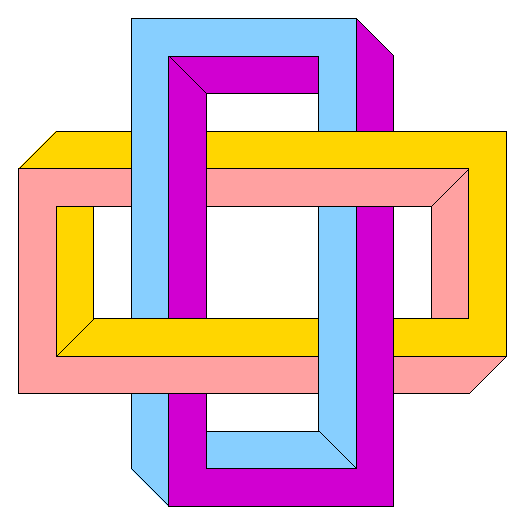
\includegraphics[width=12pt]{illusion}。

\subsection{图形驱动}\label{ssec:driver}
用户必须指定一个图形驱动以告诉图形宏包如何处理导入的图像。
目前\LaTeX{} 图形宏集支持18种不同的驱动
\footnote{
	到目前(2016年)为止,支持的驱动数已经超过了20种。——译者注
	},
不过,本文档只涉及两种最常用的驱动:
\prgname{dvips} 类型文档所用的 \prgname{dvips} 驱动
\footnote{使用 \prgname{latex} 命令将 \LaTeX{} 文件处理成 \file{dvi} 文件后,
	\prgname{dvips} 随后就将其转成 PostScript 格式。},
以及 \pdfLaTeX{} 文档所用的 \prgname{pdftex} 驱动。
如果用户使用的是这两种驱动之一,一般不用显示地指明,
因为绝大部分 \LaTeX{} 发行版中的 \file{graphics.cfg} 可以自动识别正确的驱动
\footnote{\file{graphics.cfg} 文件会检测文件是由 \prgname{latex} 还是 \prgname{pdflatex} 编译,
	对于 \prgname{latex} 会指定 \opt{dvips} 选项,
	对于 \prgname{pdflatex} 会指定 \opt{pdftex} 选项。}。

如果用户想要指定一个驱动,可以用以下三种方式
\marginpar{指定驱动}
\begin{enumerate}
	\item 默认值在 \file{graphics.cfg} 文件中指定。
	\item 任何通过 \cmd{documentclass} 的选项指定的驱动会覆盖由 \file{graphics.cfg} 文件指定的驱动。
	\item 任何由 \cmdonearg{usepackage}{graphics} 的选项指定的驱动会覆盖前两种方式指定的驱动。
\end{enumerate}

\subsection{DVIPS 模式下图像加载}
\prgname{dvips} 模式下支持最好的图像格式是 \file{eps}。
当使用 \prgname{latex} 编译文件时,下面的命令
\begin{lstlisting}[language=LaTeX]
\includegraphics{file.eps}
\end{lstlisting}
会从 \file{file.eps} 文件中按照自然大小导入图像。
如果文件名没有扩展名,
\begin{lstlisting}[language=LaTeX]
\includegraphics{file}
\end{lstlisting}
那么 \cmd{includegraphics} 会按照 \cmd{DeclareGraphicsExtensions} 扩展名列表中自动加上扩展名
(见~\pageref{ssec:deextension} 的第~\ref{ssec:deextension} 节)。

\subsection[pdfLaTeX 模式下的图像加载]{\pdfLaTeX{} 模式下的图像加载}
\pdfTeX{} 支持直接导入 \file{pdf}、\file{png}、\file{jpeg} 和 MetaPost 图像。
当使用 \prgname{pdflatex} 编译时,下面的命令
\begin{lstlisting}[language=LaTeX]
\includegraphics{file.pdf}
\includegraphics{file.png}
\includegraphics{file.jpg}
\includegraphics{file.mps}
\end{lstlisting}
会按照自然尺寸大小导入 \file{pdf} 文件 \file{file.pdf}、
\file{png} 文件 \file{file.png}、
\file{jpeg} 文件 \file{file.jpg}
以及 MetaPost 文件 \file{file.mps}。
如果文件名没有扩展名
\begin{lstlisting}[language=LaTeX]
\includegraphics{file.eps}
\end{lstlisting}
那么 \cmd{includegraphics} 会按照 \cmd{DeclareGraphicsExtensions} 扩展名列表中自动加上扩展名
(见~\pageref{ssec:deextension} 的第~\ref{ssec:deextension} 节)。

\subsection{同时供 \LaTeX{} 和 \pdfLaTeX{} 编译的文档 }\label{ssec:latexandpdflatex}
很多情况下要求文档同时可以由 \LaTeX{} 或 \pdfLaTeX{} 编译。
要求 PostScript 输出时使用 \LaTeX{} 编译和 \prgname{dvips} 驱动,
要求 \file{pdf} 输出时则使用 \pdfLaTeX{} 编译。
在这两种方式之间切换会改变两件事情。
\begin{itemize}
	\item 合适的 \pkg{graphicx} 驱动会改变。
	\item 可以直接导入的图像类型会改变。
\end{itemize}
使用如下步骤会调整这些,这样一份文档可以同时由 \LaTeX{} 和 \pdfLaTeX{} 编译。
\begin{enumerate}
	\item 对于每一份要导入的图像都创建两个副本\footnote{
		有时使用 \prgname{PurifyEPS} (见 \pageref{ssec:purifyeps} 页的第~\ref{ssec:purifyeps} 节) 可以创建一个文件并可以同时供 \LaTeX{} 和 \pdfLaTeX{} 使用。
		 Sometimes PurifyEPS (see Section 5.5 on Page 17) can be used to create a single file that can
		 be used by both L
		 A T E X and pdfL A T E X.}:
	\begin{enumerate}
		\item 一份 \file{eps} 版本,当使用 \prgname{latex} 编译时会导入。
		\item 一份 \file{png}、\file{pdf}、\file{jpeg} 或者 MetaPost 版本,
		当使用 \prgname{pdflatex} 编译时会导入。
	\end{enumerate}
	
	\item 不要在 \cmd{documentclass} 或者 \cmdonearg{usepackage}{graphicx} 命令中指定 \opt{dvips} 或者 \opt{pdftex} 选项。
	\file{graphic.cfg} 文件会自动传递合适的选项给 \pkg{graphicx} 宏包。
	
	\item 当使用 \cmd{includegraphics} 命令插图时,
	不要指定扩展名。例如
\begin{lstlisting}[language=LaTeX]
\includegraphics{graphic}
\end{lstlisting}
	定义在 \file{dvips.def} 中的默认扩展名列表会使得 \LaTeX{} 导入图像 \file{eps} 版本,
	而定义在 \file{pdftex.def} 中的默认扩展名列表会使得 \pdfLaTeX{} 导入图像的 \file{png}、\file{pdf}、\file{jpeg} 或者 MetaPost 版本
	(见~\pageref{ssec:deextension} 的第~\ref{ssec:deextension} 节)。
	
	\item 不要直接使用 \pkg{psfrag}。如果需要进行 \pkg{psfrag} 替换,
	使用~\pageref{ssec:psfrag-pdftex} 页的第~\ref{ssec:psfrag-pdftex} 节介绍的方法。
\end{enumerate}

\subsubsection{使用 \pkg{ifpdf} 宏包的条件代码}
\pkgi{ifpdf} 宏包的 \cmdi{ifpdf} 命令会检测文档是否由 \prgname{pdflatex} 编译
\footnote{
	历史上,有一种检测方法是基于 \cmd{pdfoutput} 仅在使用 \pdfLaTeX{} 时才有定义这一事实。
	然而,现在绝大部分 \TeX{} 发行版中的 \prgname{latex} 命令实际上是在 \file{dvi} 模式下执行 \pdfLaTeX{}。
	此时无论用\prgname{latex} 和 \prgname{pdflatex} 中的哪种来编译,\cmd{pdfoutput} 都有定义。
	\pkg{ifpdf} 宏包则提供了一个鲁棒的条件命令,可以判断文档是否直接处理成 \file{pdf} 文件,
	从而解决了这一问题。},
进而可以在文档中使用条件语句。

例如,为了精简扩展名列表(见第~\ref{ssec:deextension} 节),
可以用 \cmd{ifpdf} 命令来定制
\begin{lstlisting}[language=LaTeX]
\usepackage{ifpdf}
...
\ifpdf
\DeclareGraphicsExtensions{.pdf,.png,.jpg,.mps}
\else
\DeclareGraphicsExtensions{.eps}
\fi
\end{lstlisting}

如果用户想要基于条件代码来使用不同的 \cmd{documentclass} 选项,
使用如下代码可以在 \cmd{documentclass} 之前定义 \cmd{ifpdf}
\begin{lstlisting}[language=LaTeX]
\RequirePackage{ifpdf}
\ifpdf
\documentclass[pdftex]{article}
\else
\documentclass[dvips]{article}
\fi
\end{lstlisting}
这段代码当使用 \prgname{pdflatex} 时会传递 \opt{pdftex} 选项,
而使用 \prgname{latex} 编译时会传递 \opt{dvips} 选项。
不过,正如~\pageref{ssec:driver} 页的第~\ref{ssec:driver} 节所述,
这段代码实际上没有必要,因为绝大部分的发行版本会根据 \file{graphics.cfg} 文件自动处理驱动选项。


\subsection{指定宽度、高度和角度}\label{ssec:spec-width-height-angle}
如下命令
\marginpar{指定宽度}
\begin{lstlisting}
\includegraphics[width=3in]{file}
\end{lstlisting}
导入指定的图片文件,且宽度为 3英寸
\footnote{同时高度也会按相应的比例缩放——译者注}。
不过,为了使图像的页面布局更具通用性,
图片宽度最好指定为可伸缩的相对长度而不是用像3英寸这样的固定尺寸
\footnote{
	预先定义的相对长度包括:\\
	\cmd{textwidth} 是文档中正文的宽度;\\
	\cmd{linewidth} 是当前环境中一行的宽度;\\
	\texttt{em} 是当前字体大写字母M的宽度;\\
	\texttt{ex} 是当前字体小写字母x的高度。}。
例如,
\begin{itemize}
	\item 如下命令将插入的图片伸缩至和当前一行文本的宽度相同:
\begin{lstlisting}
\includegraphics[width=\linewidth]{graphic}
\end{lstlisting}
	\item 如下命令使得插入图片的宽度为当前一行文本的 $80\percent$:
\begin{lstlisting}
\includegraphics[width=0.80\linewidth]{graphic}
\end{lstlisting}
	\item 当与 \pkg{calc} 宏包配合使用时,
	如下命令可以使得插入图片的宽度比当前一行文本的宽度窄2英寸:
\begin{lstlisting}
\includegraphics[width=\linewidth-2.0in]{graphic}
\end{lstlisting}
	
\end{itemize}

类似地,如下命令
\marginpar{指定高度}
\begin{lstlisting}
\includegraphics[height=2cm]{file}
\end{lstlisting}
导入指定的图片文件,且高度为2厘米。
此外,\cmd{includegraphics} 命令还有一个 \opt{totalheight} 选项来指定整体高度
(关于高度和整体高度的定义可参见第~\pageref{sec:terminology} 页的第~\ref{sec:terminology} 节)。

\cmd{includegraphics} 命令的 \opt{angle} 选项可以指定插入图像的角度:
\marginpar{指定角度}
\begin{lstlisting}
\includegraphics[angle=45]{graphic}
\end{lstlisting}
该命令会按照原始尺寸插入图片,并且按逆时针旋转45度。

\subsubsection{同时指定角度和高度/宽度}
由于 \cmd{includegraphics} 的选项是从左到右依次解释的,
所以其中指定角度和大小顺序会导致不同的效果。例如
\begin{lstlisting}
\begin{center}
\includegraphics[angle=90,totalheight=1cm]{graphic}
\includegraphics[totalheight=1cm,angle=90]{graphic}
\end{center}
\end{lstlisting}
会生成如下结果
\begin{center}
	\includegraphics[angle=90,totalheight=1cm]{graphic}
	\includegraphics[totalheight=1cm,angle=90]{graphic}
\end{center}
第一个盒子是先旋转了90度,然后缩放使得整体高度为1厘米。
第二个盒子先缩放使得整体高度为1厘米,然后再旋转90度。
另外要注意的是,以上图形中两幅图像之间有一个空格,
因为第一行 \cmd{includegraphics} 的末尾并没有以 \texttt{\%} 结束。

\begin{table}
\centering
\kaishu
\caption{\cmd{includegraphics} 选项}\label{tab:opt}
\begin{tabular}{>{\ttfamily}l P{0.7\textwidth}}
	\toprule
	height & 图形的高度(可为任何~\TeX{}~度量单位)。 \\ \hline
	totalheight & 图形的整体高度,可为任何~\TeX{}~度量单位。 \\ \hline
	width & 图形的宽度(可为任何~\TeX{}~度量单位)。 \\ \hline
	scale & 图形的缩放因子,设定 \opt{scale=2} 会使插入图形的大小为其自然大小的两倍。 \\ \hline
	angle & 设定旋转的角度,以度为单位,逆时针方向为正。 \\ \hline
	origin & \opt{origin} 指定图形绕那一点旋转,默认是围绕参考点旋转。
		\opt{origin} 点可以与第~\ref{ssec:rotatebox}节的 \cmd{rotatebox} 命令中的一样。
	比如 \opt{origin=c} 将使图形绕它的中心旋转。  \\ \hline
	bb & 设定 BoundingBox 的值。
	例如,\opt{bb=10 20 100 200} 设定BoundingBox 的左下角在 $(10,20)$,右上角在 $(100,200)$。\par
	因为 \cmd{includegraphics} 会自动从 \file{eps} 文件中读入BoundingBox值,
	所以一般不用\opt{bb} 这个选项。
	但它在 \file{eps} 文件中的 BoundingBox 丢失或不准确时还是很有用的。 \\ 
	\bottomrule
\end{tabular}
\end{table}

\begin{table}
\centering
\caption{\cmd{includegraphics} 裁剪选项}\label{tab:cropopt}
\kaishu
\begin{tabular}{>{\ttfamily}l P{0.7\textwidth}}
	\toprule
	viewpoint & 指定图像可以被看到的部分。
	如同 BoundingBox 一样,这个区域由四个数字决定,分别是左下角和右上角的坐标。
	这里的坐标是以 BoundingBox 左下角为起点的相对坐标。
	
	例如,如果图像的 BoundingBox 的值是 \texttt{50	50 410 302},
	那么 \texttt{viewpoint=50 50 122 122} 将显示以图像左下角为左下角的一英寸大小的正方形区域。
	而 \texttt{viewpoint=338 230 410 302} 则会显示以图形的右上角为右上角的一英寸大小的正方形区域。
	
	必须使用\opt{clip} 选项(见表~\ref{tab:boolopt})来阻止显示视图以外的图形部分。 \\ \hline
	trim & 显示部分图像的另一种方法。
	所给出的四个数字分别代表了从左、下、右、上被截去的值。
	正数代表从此方向截去的大小,而负数则代表从此方向加上的大小。
	
	例如,\opt{trim=1 2 3 4} 代表图像的左边截去1 \texttt{bp},
	下边截去2 \texttt{bp},右边截去3 \texttt{bp},上边截去4 \texttt{bp}。
	
	必须使用\opt{clip} 选项(见表~\ref{tab:boolopt})来阻止显示被截去的部分。 \\ \bottomrule
\end{tabular}
\end{table}

\begin{table}
\centering
\caption{\cmd{includegraphics} 布尔型选项}\label{tab:boolopt}
\begin{tabular}{>{\ttfamily}l P{0.7\textwidth} }
	\toprule
	clip & 指定 \opt{clip=false} 会显示整个的图形,即使有些部分在视图之外。(默认值)
	
	指定 \opt{clip=true} 时将不显示图形在视图之外的部分。 \\ \hline
	draft & 当使用\opt{draft} 或 \opt{draft=true} 选项将阻止图像的导入。
	此时在插图的位置只显示图像的BoundingBox和文件名,
	这会加快文档的显示和打印速度。
	使用 \opt{draft=false} 则会显示图像。
	
	如果使用 \opt{draft} 宏包选项 \cmdtwoargs{usepackage}{draft}{graphicx},
	那么文档中的所有图像都以\opt{draft} 方式插入。  \\ \hline
	keepaspectratio & 在没有设定\opt{keepaspectratio} 选项时,
	如果同时给定图像的宽度和高度/整体高度,
	那么为了满足所设定的高和宽,图像的缩放可能会失真变形。
	
	在设定\opt{keepaspectratio} 选项后,给定图像的宽度和高度/整体高度时,
	图像会在保持原有的宽高比例下缩放,尽可能使得图像满足所设定的高和宽,
	但是图像的实际宽高不会超出设置的值。 \\ \bottomrule
\end{tabular}
\end{table}


\subsection{一些例子}

下面是一些使用 \cmd{includegraphics} 命令来插入图形的例子。
\footnote{
	本小节来自于王磊在旧版本的中译本《\LaTeXe{} 插图指南》中额外补充的内容。——译者注}
这里为方便起见,定义水平线 \cmd{HR} 为
\begin{lstlisting}
\newcommand{\HR}{\rule{1em}{0.4pt}}
\end{lstlisting}

\ifpdf\else %因为使用pdflatex不支持clip.所以省去。
在下面的几个例子中可以看到使用\opt{bb,clip,viewport} 和\opt{trim}的效果。

\hspace{-1cm}\begin{minipage}[c]{.5\textwidth}
	左\HR%
	\fbox{%
		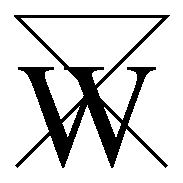
\includegraphics[bb=120 120 150 200]{w.eps}}%
	\HR 右
	\qquad
	左\HR%
	\fbox{%
		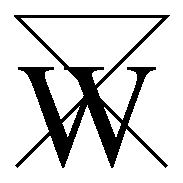
\includegraphics[bb=120 120 150 200,clip]{w.eps}}%
	\HR 右
\end{minipage}%
\begin{minipage}[c]{.5\textwidth}
	\begin{Verbatim}[frame=lines,label=\colorbox{green}{\small 例一},labelposition=topline,]
	左\HR\fbox{%
	\includegraphics
	[bb=120 120 150 200]%
	{w.eps}}%
	\HR 右
	\qquad
	左\HR\fbox{%
	\includegraphics
	[bb=120 120 150 200,clip]%
	{w.eps}}%
	\HR 右
	\end{Verbatim}
\end{minipage}

\hspace{-1.5cm}\begin{minipage}[c]{.65\textwidth}
	左\HR\fbox{%
		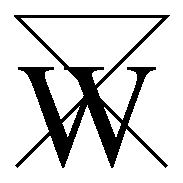
\includegraphics[viewport=20 20 50 100,clip]{w}}%
	\HR 右
	\qquad
	左\HR\fbox{%
		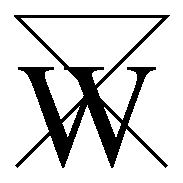
\includegraphics[trim=5 5 10 10,clip]{w}}%
	\HR 右
\end{minipage}%
\hspace{-1cm}\begin{minipage}[c]{.5\textwidth}
	\begin{Verbatim}[frame=lines,label=\colorbox{green}{\small 例二},labelposition=topline]
	左\HR\fbox{%
	\includegraphics
	[viewport=20 20 50 100,clip]%
	{w.eps}}%
	\HR 右
	\qquad
	左\HR\fbox{%
	\includegraphics
	[trim=5 5 10 10,clip]%
	{w.eps}}
	\HR 右
	\end{Verbatim}
	\par\vspace{0pt}
\end{minipage}
\fi

在下面的几个例子中,可以比较以下使用 \opt{scale,width,height,angle} 以及 \opt{keepaspectratio} 选项及其不同的顺序所得到的不同效果。

\begin{minipage}[t]{.45\textwidth}
	\vspace{0pt}
	左\HR\fbox{%
		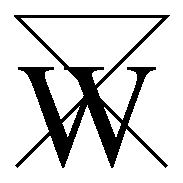
\includegraphics[scale=.5]{w}}\HR 右
\end{minipage}%
\hspace{-.5cm}\begin{minipage}[t]{.5\textwidth}
	\vspace{0pt}
	\begin{Verbatim}[frame=lines,label=\colorbox{green}{\small 例一},labelposition=topline]
	左\HR\fbox{%
	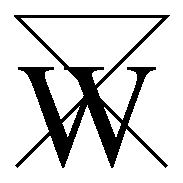
\includegraphics
	[scale=.5]{w.eps}%
	\HR 右
	\end{Verbatim}
\end{minipage}

\begin{minipage}[c]{.45\textwidth}
	左\HR\fbox{%
		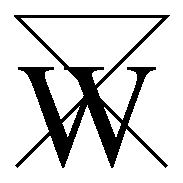
\includegraphics[width=10mm]{w}}\HR 右
\end{minipage}%
\hspace{-.5cm}\begin{minipage}[c]{.5\textwidth}
	\begin{Verbatim}[frame=lines,label=\colorbox{green}{\small 例二},labelposition=topline]
	左\HR\fbox{%
	\includegraphics%
	[width=10mm]{w.eps}%
	\HR 右
	\end{Verbatim}
\end{minipage}

\begin{minipage}[c]{.45\textwidth}
	左\HR\fbox{%
		\includegraphics[height=20mm,width=30mm]%
		{w}}\HR 右
\end{minipage}%
\hspace{-.5cm}\begin{minipage}[c]{.5\textwidth}
	\begin{Verbatim}[frame=lines,label=\colorbox{green}{\small 例三},labelposition=topline]
	左\HR\fbox{%
	\includegraphics
	[height=20mm,width=30mm]%
	{w.eps}}\HR 右
	\end{Verbatim}
\end{minipage}

\begin{minipage}[c]{.45\textwidth}
	左\HR\fbox{%
		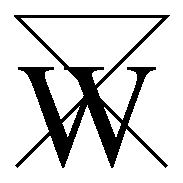
\includegraphics[height=20mm,width=30mm,%
		keepaspectratio]{w}}\HR 右
\end{minipage}%
\hspace{-.5cm}\begin{minipage}[c]{.5\textwidth}
	\begin{Verbatim}[frame=lines,label=\colorbox{green}{\small 例四},labelposition=topline]
	左\HR\fbox{%
	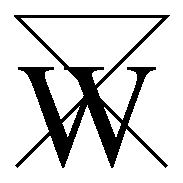
\includegraphics
	[height=20mm,width=30mm,%
	keepaspectratio]{w.eps}}%
	\HR 右
	\end{Verbatim}
\end{minipage}

\begin{minipage}[c]{.45\textwidth}
	左\HR\fbox{%
		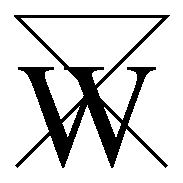
\includegraphics[angle=-45]{w}}\HR 右
\end{minipage}%
\hspace{-.5cm}\begin{minipage}[c]{.5\textwidth}
	\begin{Verbatim}[frame=lines,label=\colorbox{green}{\small 例五},labelposition=topline]
	左\HR\fbox{%
	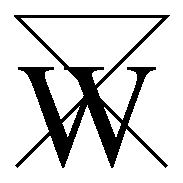
\includegraphics
	[angle=-45]{w.eps}}%
	\HR 右
	\end{Verbatim}
\end{minipage}

\begin{minipage}[c]{.45\textwidth}
	左\HR\fbox{%
		\includegraphics[angle=-45,width=30mm]%
		{w}}\HR 右
\end{minipage}%
\hspace{-.5cm}\begin{minipage}[c]{.5\textwidth}
	\begin{Verbatim}[frame=lines,label=\colorbox{green}{\small 例六},labelposition=topline]
	左\HR\fbox{%
	\includegraphics
	[angle=-45,width=30mm]%
	{w.eps}}\HR 右
	\end{Verbatim}
\end{minipage}

\hspace{-1cm}\begin{minipage}[c]{.45\textwidth}
	左\HR\fbox{%
		\includegraphics[width=30mm,angle=-45]%
		{w}}\HR 右
\end{minipage}%
\begin{minipage}[c]{.5\textwidth}
	\begin{Verbatim}[frame=lines,label=\colorbox{green}{\small 例七},labelposition=topline]
	左\HR\fbox{%
	\includegraphics
	[width=30mm,angle=-45]%
	{w.eps}}\HR 右
	\end{Verbatim}
\end{minipage}

\begin{minipage}[c]{.45\textwidth}
	左\HR\fbox{%
		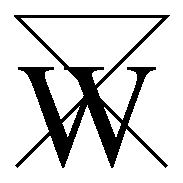
\includegraphics[angle=-60,totalheight=15mm]{w}}%
	\HR 右
\end{minipage}%
\hspace{-.5cm}\begin{minipage}[c]{.5\textwidth}
	\begin{Verbatim}[frame=lines,label=\colorbox{green}{\small 例八},labelposition=topline]
	左\HR\fbox{%
	\includegraphics
	[angle=-60,totalheight=15mm]%
	{w.eps}}%
	\HR 右
	\end{Verbatim}
\end{minipage}

\begin{minipage}[c]{.45\textwidth}
	左\HR\fbox{%
		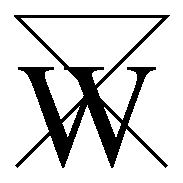
\includegraphics[angle=-60,totalheight=20mm,width=30mm]{w}}%
	\HR 右
\end{minipage}%
\hspace{-.5cm}\begin{minipage}[c]{.5\textwidth}
	\begin{Verbatim}[frame=lines,label=\colorbox{green}{\small 例九},labelposition=topline]
	左\HR\fbox{%
	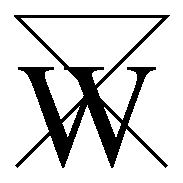
\includegraphics
	[angle=-60,totalheight=20mm,%
	width=30mm]{w.eps}}%
	\HR 右
	\end{Verbatim}
\end{minipage}

\begin{minipage}[c]{.45\textwidth}
	左\HR\fbox{%
		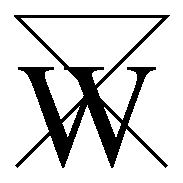
\includegraphics[angle=-60,totalheight=20mm,width=30mm,keepaspectratio]{w}}%
	\HR 右
\end{minipage}%
\hspace{-.5cm}\begin{minipage}[c]{.5\textwidth}
\begin{Verbatim}[frame=lines,label=\colorbox{green}{\small 例十},labelposition=topline]
	左\HR\fbox{%
	\includegraphics
	[angle=-60,totalheight=20mm,%
	width=30mm,keepaspectratio]%
	{w.eps}}%
	\HR 右
\end{Verbatim}
\end{minipage}

\section{旋转和缩放对象}\label{sec:scalerotate}
除了 \cmd{includegraphics}命令外,
\pkg{graphicx} 宏包还提供了另外四个命令用来旋转和缩放任意的 \LaTeX{} 对象,例如文本、图像等。
\begin{lstlisting}
\scalebox{水平缩放因子}[垂直缩放因子]{对象}
\resizebox{宽度}{高度}{对象}
\resizebox*{宽度}{整体高度}{对象}
\rotatebox[选项]{角度}{对象}
\end{lstlisting}

因为 \pkg{graphicx} 包的 \cmd{includegraphics} 已经带有 \opt{angle}、\opt{width} 等支持旋转和缩放的选项,
所以本节介绍的这几个命令很少在插图时使用。例如:
\begin{lstlisting}
\includegraphics[scale=2]{file.eps}
\includegraphics[width=4in]{file.eps}
\includegraphics[angle=45]{file.eps}
\end{lstlisting}
上述命令和下面的命令等到的结果是相同的。
\begin{lstlisting}
\scalebox{2}{\includegraphics{file.eps}}
\resizebox{4in}{!}{\includegraphics{file.eps}}
\rotatebox{45}{\includegraphics{file.eps}}
\end{lstlisting}

尽管结果相同,但在最好还是用前一种方法,
因为它的速度更快,而且生成的 PostScript 和 \file{pdf} 效率更高。

\subsection{scalebox 命令}\label{ssec:scalebox}
语法:
\begin{lstlisting}
\scalebox{水平缩放因子}[垂直缩放因子]{对象}
\end{lstlisting}

\cmdi{scalebox} 命令对其作用的对象进行缩放,
使得缩放后对象的宽度为原始宽度与\texttt{水平缩放因子}之积,高度为原始高度与\texttt{垂直缩放因子}之积。
如果\texttt{垂直缩放因子}没有给出,那么默认取为\texttt{水平缩放因子},
以保持原始的宽高比进行缩放。
如果缩放因子为负值,则对对象进行翻转。下面是几个例子

\hspace{-1.5cm}\begin{minipage}[b]{.5\textwidth}
	\begin{center}
		\color{blue}{\CJKfamily{kai}
			\scalebox{2}{%
				这是放大的文字} \\
			这是正常的文字 \\
			\scalebox{.5}{%
				这是缩小的文字}}
	\end{center}
	\par\vspace{0pt}
\end{minipage}%
\begin{minipage}[b]{.5\textwidth}
	\begin{Verbatim}[formatcom=\color{VerbatimColor}\CJKfamily{kai}]
	\scalebox{2}{这是放大的文字} \\
	这是正常的文字  \\
	\scalebox{.5}{这是缩小的文字}
	\end{Verbatim}
	\par\vspace{0pt}
\end{minipage}

\hspace{-1.5cm}\begin{minipage}[b]{.5\textwidth}
	\color{blue}{\CJKfamily{kai}
		\framebox{\scalebox{2}{%
				\parbox{.5in}{放大 \\ 和 \\ 缩小}}}
		\framebox{\scalebox{2}[1.5]{%
				\parbox{.5in}{放大 \\ 和 \\ 缩小}}}}
	\par\vspace{0pt}
\end{minipage}%
\begin{minipage}[b]{.5\textwidth}
	\begin{Verbatim}[formatcom=\color{VerbatimColor}\CJKfamily{kai}]
	\framebox{\scalebox{2}{%
	\parbox{.5in}{放大 \\ 和 \\ 缩小}}}
	\framebox{\scalebox{2}[1.5]{%
	\parbox{.5in}{放大 \\ 和 \\ 缩小}}}
	\end{Verbatim}
	\par\vspace{0pt}
\end{minipage}

\hspace{-1.5cm}\begin{minipage}[b]{.5\textwidth}
	\begin{center}
		\color{blue}{\texttt{%
				China? \scalebox{-1}[1]{China?} \\
				China? \scalebox{1}[-1]{China?} \\
				China? \scalebox{-1}[-1]{China?} \\
				China? \scalebox{-1}{China?}}}
	\end{center}
	\par\vspace{0pt}
\end{minipage}%
\begin{minipage}[b]{.5\textwidth}
	\begin{Verbatim}
	China? \scalebox{-1}[1]{China?} \\
	China? \scalebox{1}[-1]{China?} \\
	China? \scalebox{-1}[-1]{China?} \\
	China? \scalebox{-1}{China?}}
	\end{Verbatim}
	\par\vspace{0pt}
\end{minipage}

\subsection{resizebox 命令}\label{ssec:resizebox}
语法:
\begin{lstlisting}
\resizebox{宽度}{高度}{对象}
\resizebox*{宽度}{整体高度}{对象}
\end{lstlisting}

\cmdi{resizebox} 命令将对象的大小改变为给定值。
如果\texttt{宽度}或\texttt{高度}中的任一项用 \texttt{!} 给出,
那么缩放时会保持原有的宽高比。
例如:
\begin{lstlisting}
\resizebox{2in}{!}{argument}
\end{lstlisting}
将对象的宽度改变为2英寸,同时保持宽高比。

标准的 \LaTeXe{} 长度命令 \cmd{height}、\cmd{width}、\cmd{totalheight}、\cmd{depth} 可用来表示对象的原始尺寸。
因此,
\begin{lstlisting}
\resizebox{2in}{\height}{argument}
\end{lstlisting}
使得对象的宽度改变为 2 英寸但保持原有高度不变。 

除了以外,
命令 \cmdi{reseizebox*} 与 \cmd{resizebox} 几乎是相同的
不同之处仅在于第二个参数表示对象的全部高度
(关于高度和整体高度的定义见第~\ref{sec:terminology} 节,
关于 \opt{height} 和 \opt{totalheight} 选项的比较见第~\ref{ssec:diffheight} 节。)

下面是几个例子:

\hspace{-1.5cm}\begin{minipage}[b]{.5\textwidth}
	\begin{center}
		\color{blue}{\CJKfamily{kai}
			\framebox{\resizebox{5mm}{!}{%
					\parbox{14mm}{选项 \\ 角度 \\ 对象}}}
			\framebox{\resizebox{!}{10mm}{%
					\parbox{14mm}{选项 \\ 角度 \\ 对象}}}}
		\par\vspace{0pt}
	\end{center}
\end{minipage}%
\hspace{-1cm}\begin{minipage}[b]{.5\textwidth}
	\begin{Verbatim}[formatcom=\color{VerbatimColor}\CJKfamily{kai}]
	\framebox{\resizebox{5mm}{!}{%
	\parbox{14mm}{选项 \\ 角度 \\ 对象}}}
	\framebox{\resizebox{!}{10mm}{%
	\parbox{14mm}{选项 \\ 角度 \\ 对象}}}
	\end{Verbatim}
	\par\vspace{0pt}
\end{minipage}

\hspace{-2cm}\begin{minipage}[b]{.5\textwidth}
	\begin{center}
		\color{blue}{\CJKfamily{kai}
			\resizebox*{2cm}{3cm}{\LaTeX{}~图形} \\
			\resizebox*{2cm}{1cm}{\LaTeX{}~图形}}
		\par\vspace{0pt}
	\end{center}
\end{minipage}%
\begin{minipage}[b]{.5\textwidth}
	\begin{Verbatim}[formatcom=\color{VerbatimColor}\CJKfamily{kai}]
	\resizebox*{2cm}{3cm}{\LaTeX{}~图形} \\
	\resizebox*{2cm}{1cm}{\LaTeX{}~图形}
	\end{Verbatim}
	\par\vspace{0pt}
\end{minipage}

\subsection{rotatebox 命令}\label{ssec:rotatebox}
语法:
\begin{lstlisting}
\rotatebox[选项]{角度}{对象}
\end{lstlisting}
\cmdi{rotatebox} 将对象旋转一给定度数的角度,逆时针方向为正。
默认\texttt{选项}下对象绕它的参考点旋转。
\cmd{rotatebox} 命令中\texttt{选项} 允许对象绕给定的点来旋转。
\begin{enumerate}
	\item 给定\opt{[x=xdim,y=ydim]},则对象旋转所绕的点相对于参考点的
	坐标为 $(\mathtt{xdim}, \mathtt{ydim})$。
	\item \opt{origin} 选项可以指定12个特殊点其中之一(见图~\ref{fig:rotatepoint})。
\end{enumerate}

\opt{origin} 点的水平位置由\opt{lcr} (分别代表左、中、右)三个字母其中之一确定,
垂直位置则由\opt{t,c,B,b}~(分别代表顶部、中部、基线、底部)四个字母中的一个来确定。
例如:
\begin{description}
	\item [\opt{[rb]}] 右下角。
	\item [\opt{[lt]}] 左上角。
	\item [\opt{[cB]}] 图形基线的中点。
\end{description}

\paragraph{几点说明:}
\begin{itemize}
	\item 标记字母的顺序并不重要,\opt{[br]} 等同于 \opt{[rb]}。
	\item \opt{c}~代表水平位置的中点还是垂直位置的中点由和它一起的标记字母来决定。
	\item 如果只给出一个标记字母,那么另一个将被假设为 \opt{c}。
	即,\opt{[c]} 等于\opt{[cc]},\opt{[l]}等于\opt{[lc]},\opt{[t]}等于\opt{[ct]},等等。
\end{itemize}

\begin{figure}
	\centering
	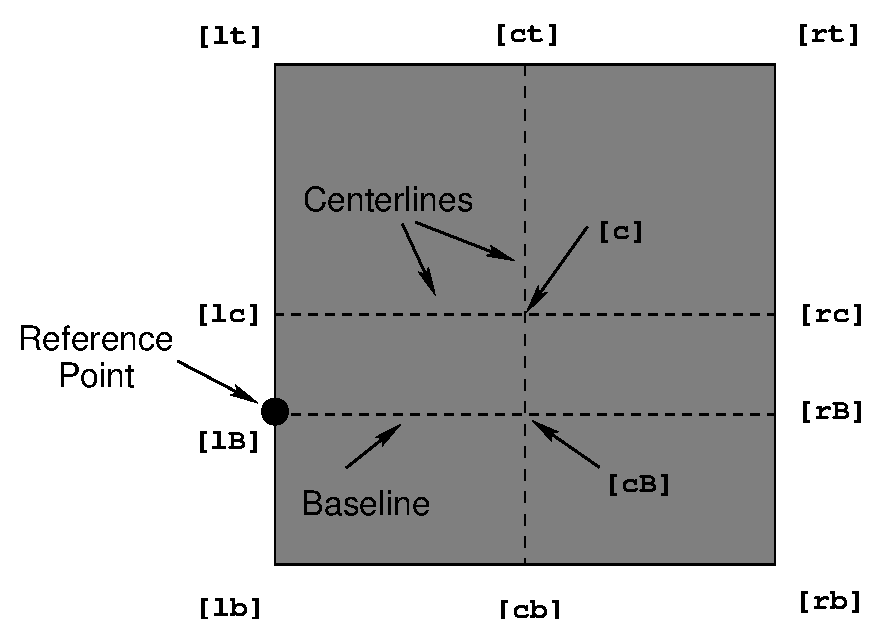
\includegraphics[width=.6\textwidth]{orig-point}
	\caption{可用的 \opt{origin} 点}\label{fig:rotatepoint}
\end{figure}

下面是一个例子:

\hspace{-1.5cm}\begin{minipage}[b]{.5\textwidth}
	\begin{center}
		\setlength{\fboxsep}{0mm}
		\newcommand{\MyRot}[1]{%
			\fbox{\rotatebox{#1}{旋转~$#1^\circ$}}}
		\color{blue}{\CJKfamily{kai}
			\MyRot{0} \MyRot{45} \MyRot{90}
			\MyRot{135} \MyRot{180} \MyRot{225}}
	\end{center}
	\par\vspace{0pt}
\end{minipage}%
\begin{minipage}[b]{.5\textwidth}
	\begin{Verbatim}[formatcom=\color{VerbatimColor}\CJKfamily{kai}]
	\setlength{\fboxsep}{0mm}
	\newcommand{\MyRot}[1]{%
	\fbox{\rotatebox{#1}{旋转~$#1^\circ$}}}
	\MyRot{0} \MyRot{45} \MyRot{90}
	\MyRot{135} \MyRot{180} \MyRot{225}
	\end{Verbatim}
	\par\vspace{0pt}
\end{minipage}


\section{高级插图命令}\label{sec:adgraphcmd}
本节描述了一些 \LaTeXe{} 图形宏包套件的高级命令,
用于下述情形。
\begin{enumerate}
	\item 当使用没有扩展名的文件名时。如:
\begin{lstlisting}
\includegraphics{file}
\end{lstlisting}

	\item 当使用压缩的\file{eps} 图形文件时。见第~\ref{ssec:compresseps}~节。
	\item 当使用非\file{eps} 格式的图形文件时。见第~\ref{ssec:noneps}~节。
\end{enumerate}
在这些情况下,\LaTeX{} 为了处理由 \cmd{includegraphics} 所引入的文件,
就需要用 \cmdi{DeclareGraphicsRule} 和 \cmdi{DeclareGraphicsExtensions} 命令来控制。
\begin{itemize}
	\item \cmd{DeclareGraphicsExtensions} 命令指定了在没有提供图形文件扩展名的情况下,
	\LaTeX{} 将自动为其加上的扩展名列表(如~\file{.eps}、\file{.ps}、\file{.eps.gz} 等)。
	\item \cmd{DeclareGraphicsRule} 命令指定了对图形文件执行的命令。
	执行这一命令要求操作系统支持管道功能,比如 Unix 等操作系统,而DOS则不行。
	
	若将此命令指定为一解压缩命令,那么就可以使用压缩的 \file{eps} 图形文件。
	若将此命令指定为一图形格式转换命令,那么就可以使用非\file{eps} 格式的图形文件。
\end{itemize}

\subsection{DeclareGraphicsExtensions 命令}\label{ssec:deextension}
\cmd{DeclareGraphicsExtensions} 命令告诉 \LaTeX{},
若~\cmd{includegraphics}~命令所引入的文件没有提供扩展名,
将试图为其自动加上什么样的扩展名。

为方便起见,在选择图形驱动
\footnote{
	指定一个图形驱动选项如 \cmdtwoargs{usepackage}{dvips}{graphics} 将会覆盖掉在~\texttt{graphics.cfg} 中设定的缺省驱动选项——旧译本注。}
时,就已经有一个相应的预设扩展名集。
举例来说,如果选择 \prgname{dvips} 作为图形驱动,
那么默认会使用下列图形文件扩展名(在~\file{dvips.def}~中定义):
\begin{lstlisting}
\DeclareGraphicsExtensions{.eps,.ps,.eps.gz,.ps.gz,.eps.Z}
\end{lstlisting}

如果 \pkg{graphicx} 宏包使用 \prgname{pdftex} 驱动,
那么默认会使用下列图形文件扩展名(在 \file{pdftex.def} 中定义)
\footnote{
	实际上在最新版本(2016年)中,\file{dvips.def} 中定义扩展名的方式为
\begin{lstlisting}
%\def\Gin@extensions{.eps,.ps,.eps.gz,.ps.gz,.eps.Z,.mps}
\end{lstlisting}
	\file{pdftex.def} 中定义扩展名的方式为
\begin{lstlisting}
\def\Gin@extensions{.png,.pdf,.jpg,.mps,.jpeg,.PNG,.PDF,.JPG,.JPEG}
\end{lstlisting}
	——译者注}:
\begin{lstlisting}
\DeclareGraphicsExtensions{.png,.pdf,.jpg,.mps}
\end{lstlisting}

在 \opt{dvips} 图像扩展名列表中,
\cmdonearg{includegraphics}{file} 首先寻找 \file{file.eps},
其次是 \file{file.ps},再其次是 \texttt{file.eps.gz},直到找到一个文件。
相应地,可以用
\begin{lstlisting}
\includegrapincs{file}
\end{lstlisting}
取代
\begin{lstlisting}
\includegrapincs{file.eps}
\end{lstlisting}
这样做的好处是如果以后决定压缩 \file{file.eps},也无须更改 \LaTeX{} 文件。
无后缀名的方式使得可以同时使用 \LaTeX{} 和 \pdfLaTeX{} 编译文档,
见第~\pageref{ssec:latexandpdflatex} 页的~\ref{ssec:latexandpdflatex} 节。
然而,这种无后缀名的方式可能会加剧内存池空间问题,详见下面的~\ref{sssec:poolspaceproblem} 小节。

\subsubsection{无扩展名的文件}
需要注意的是,
\begin{lstlisting}
\includegrapincs{file}
\end{lstlisting}
不会试图寻找~\file{file},
除非空扩展名列表中包含空的扩展名 \verb+{}+。
例如:
\begin{lstlisting}
\DeclareGraphicsExtensions{.eps,.eps.gz,{}}
\end{lstlisting}
将试图在没找到 \file{file.eps} 和 \file{file.eps.gz} 的情况下寻找 \file{file}。

由于默认的扩展名列表中不包含空扩展名,
如果想要使用无扩展名文件的话,
必须使用 \cmd{DeclareGraphicsExtensions} 命令定义一个包含空扩展名的列表。

\subsubsection{池空间问题}\label{sssec:poolspaceproblem}

不给出扩展名而靠 \LaTeX{} 从 \cmd{DeclareGraphicsExtensions} 的扩展名列表中选择正确的扩展名可能
加剧池空间问题(见第~\ref{ssec:poolspace}~节)。
如果有池空间问题的话,应当使用 \cmd{DeclareGraphicsExtensions} 指定的扩展名数目尽可能小。如:
\begin{lstlisting}
\DeclareGraphicsExtensions{.eps,.eps.gz}
\end{lstlisting}


\subsection{DeclareGraphicsRule 命令}\label{ssec:derule}
\cmdi{DeclareGraphicsRule} 命令指定 \cmd{includegraphics} 如何按照扩展名
来对操作图像文件。语法为
\begin{lstlisting}
\DeclareGraphicsRule{ext}{type}{sizefile}{command}
\end{lstlisting}
例如,如下命令
\begin{lstlisting}
\DeclareGraphicsRule{.eps.gz}{eps}{.eps.bb}{`gunzip -c #1}
\end{lstlisting}
指定任何以 \file{.eps.gz} 为扩展名的文件为压缩的\file{eps} 文件,
该文件的 BoundingBox 信息存放在扩展名为 \file{.eps.bb} 的文件中,
并用命令 \texttt{gunzip -c} 来解压缩
(因为 \LaTeX{} 不能从压缩文件中读取 BoundingBox~信息,
所以 BoundingBox 行必须存放到非压缩文件中)。

可以允许有多个 \cmd{DeclareGraphicsRule} 命令。

\cmd{DeclareGraphicsRule} 命令允许使用 \texttt{*} 代表任何未知扩展名,
例如:
\begin{lstlisting}
\DeclareGraphicsRule{*}{eps}{*}{}
\end{lstlisting}
会导致所有未知扩展名的文件都被认为是 \file{eps} 文件,
比方说 \file{file.EPS} 就被当做\file{eps} 文件。

\begin{table}
	\centering
	\caption{\cmd{DeclareGraphicsRule} 的选项}\label{tab:DeclaregruleArgs}
	\kaishu 
	\begin{tabular}{>{\ttfamily}l  P{0.7\textwidth}}
		\toprule
		ext & 文件的扩展名。 \\ \hline
		type & 扩展名所对应的图像类型。 \\ \hline
		sizefile & 包含图像 BoundingBox 信息的文件的扩展名。
		如果这一选项为空,
		那么必须要在 \cmd{includegraphics} 命令中给定 \opt{bb} 选项的值。 \\ \hline
		command & 作用于图像文件的命令,此项常为空。
		命令前必须有一个前单引号(键盘上数字键 \texttt{1} 的左侧键——译者注),
		注意不是常用的后单引号。
		目前为止,只有 \prgname{dvips} 能够执行这样的命令。
		参见第~\ref{sec:noneps}~节关于如何用这样的命令来处理非 \file{eps} 格式图像和压缩的 \file{eps} 图像的例子。\\
		\bottomrule
	\end{tabular}
\end{table}

文件的扩展名定义为文件名里第一个句点以后的部分,
\marginpar{文件名中的句点}
这样做是为了可以将 \file{.eps.gz} 结尾的文件识别成压缩的\file{eps} 文件。
为了避免混淆,文件的基本名中不要使用句点。
例如,指定文件 \file{file.name.eps.gz} 会让 \cmd{includegraphics} 寻找扩展名为 \file{.name.eps.gz} 所对应的图像规则。
由于这样的规则很有可能不存在,结果导致使用未知扩展名所对应的规则。
例外的情形是该文件的格式正好是缺省格式,
如果未知扩展名的文件都被认为是 \file{eps} 文件,
那么 \file{file.name.eps} 就恰巧能被正确地识别。

为方便起见,根据不同的图形驱动选项,
\marginpar{预定义命令}
已经预定义了不同的缺省图像规则。
例如使用 \opt{dvips} 图形驱动选项时,文件 \file{dvips.def} 定义了如下缺省图形规则
\footnote{
	实际上 \file{dvips.def} 的代码并没有使用 \cmd{DeclareGraphicsRule},
	不过效果是一样。}:
\begin{lstlisting}
\DeclareGraphicsRule{.eps}{eps}{.eps}{}
\DeclareGraphicsRule{.ps}{eps}{.ps}{}
\DeclareGraphicsRule{.pz}{eps}{.bb}{`gunzip -c #1}
\DeclareGraphicsRule{.eps.Z}{eps}{.eps.bb}{`gunzip -c #1}
\DeclareGraphicsRule{.ps.Z}{eps}{.ps.bb}{`gunzip -c #1}
\DeclareGraphicsRule{.eps.gz}{eps}{.eps.bb}{`gunzip -c #1}
\DeclareGraphicsRule{.ps.gz}{eps}{.ps.bb}{`gunzip -c #1}
\DeclareGraphicsRule{.pcx}{bmp}{}{}
\DeclareGraphicsRule{.bmp}{bmp}{}{}
\DeclareGraphicsRule{.msp}{bmp}{}{}
\DeclareGraphicsRule{*}{eps}{*}{}
\end{lstlisting}
前面两个命令定义扩展名为 \file{.eps} 和 \file{.ps} 的文件为 \file{eps} 文件,
它们后面的五个命令定义了压缩 \file{eps} 文件的扩展名和解压命令,
接下来的三个命令定义了位图文件 \file{pcx}、\file{bmp}、\file{msp} 的扩展名,
最后一个命令设定未知扩展名的文件按照 \file{eps} 文件处理。

如果使用 \pdfTeX 引擎,那么 \file{pdftex.def} 缺省定义了以下的图形规则
\footnote{
	\file{pdftex.def} 实际上先检查 \pdfTeX{} 的版本,
	然后根据不同版本的处理方式定义相应的图形规则。}:
\begin{lstlisting}
\DeclareGraphicsRule{.png}{png}{.png}{}
\DeclareGraphicsRule{.pdf}{pdf}{.pdf}{}
\DeclareGraphicsRule{.jpg}{jpg}{.jpg}{}
\DeclareGraphicsRule{.mps}{mps}{.mps}{}
\end{lstlisting}
这样就指定了 \pdfTeX{} 支持的图像格式的处理方式。

\clearpage
\endinput



%part3.tex

\part{\LaTeX{}图形命令的使用}

\section{水平间距和居中}\label{sec:center}

\subsection{水平居中}\label{ssec:hcenter}

图形的放置位置由当前文本的排列方式所决定。为使图形居中放置,可将其
放入一个居中(center)环境中。

\begin{Verbatim}[xleftmargin=1cm]
\begin{center}
   \includegraphics[width=2in]{graphic.eps}
\end{center}
\end{Verbatim}

如果将~\cmd{includegraphics}~命令放入一个环境中(\texttt{minipage}~或
~\texttt{figure}),用~\ci{centering}~可将其后的内容居中排列。例如:

\begin{Verbatim}[xleftmargin=1cm]
\begin{figure}
   \centering
   \includegraphics[width=2in]{graphic.eps}
\end{figure}
\end{Verbatim}
就等同于
\begin{Verbatim}[xleftmargin=1cm]
\begin{figure}
\begin{center}
   \includegraphics[width=2in]{graphic.eps}
\end{center}
\end{figure}
\end{Verbatim}

这里推荐使用~\cmd{centering},因为~\verb+\begin{center}+~会使图形上下
方的垂直间距增加一倍(~\texttt{figure}~环境带有的间距加上~\texttt{center}~环境
带有的间距)。若希望有特殊的垂直间距,可使用第~\ref{sec:vspace}~节介绍的命令。

\cmd{psfig}~和~\cmd{epsfbox}~命令\marginpar{\CJKfamily{kai}\bfseries 过时的用法}
的缺陷让它们很难使图形居中排列。作为一种解决办法,使用了~\TeX{}~
命令~\ci{centerline}~和~\ci{leavevmode}。而~\cmd{includegraphics}~命令
已克服了这些缺陷,允许直接与~\cmd{centering}~命令一起使用或用在~\texttt{center}
~环境中,因此也就不需再使用~\cmd{centerline}~和~\cmd{leavevmode}了。

\subsection{水平间距}\label{ssec:hspace}

\LaTeX{}~在排列图形的时候实际上与排列其它的像文字这样的对象是一样的,
了解到这一点很重要。举例来说,如果行尾不是以~\%~结束的话,~\LaTeX{}~会
自动在两行之间加进一个字符的水平间距。像:
\begin{Verbatim}[xleftmargin=1cm,formatcom=\CJKfamily{kai}\color{VerbatimColor}]
朋友
你好
\end{Verbatim}
在输出结果中``{\CJKfamily{kai}朋友}''~和~``{\CJKfamily{kai}你好}''~之间
会有一个字符的水平间距。

\begin{Verbatim}[xleftmargin=1cm]
\includegraphics{file.eps}
\includegraphics{file.eps}
\end{Verbatim}
则在图形之间有一个字符的水平间距。在第一行的行尾加上一个~\%~
\begin{Verbatim}[xleftmargin=1cm]
\includegraphics{file.eps}%
\includegraphics{file.eps}
\end{Verbatim}
就会使图形之间没有水平间距。如果需要,可用~\ci{hspace}~命令在图形之间
加进指定长度\realfootnote{用~\cmd{textwidth}~或~\cmd{em}~等的函数作为~\cmd{hspace}
~的参数,而不是采用一固定度量,可提高文档的通用性。}或用~\ci{hfill}~来
加进一个可填充可能的间距的橡皮长度。例如:
\begin{Verbatim}[xleftmargin=1cm]
\includegraphics{file.eps}\hfill\includegraphics{file.eps}
\end{Verbatim}
将两个图形尽量向左右分开。而
\begin{Verbatim}[xleftmargin=1cm]
\hfill\includegraphics{file.eps}%
\hfill\includegraphics{file.eps}\hspace*{\fill}
\end{Verbatim}
使得图形的两边和中间的间距都相等。由于换行符前的~\cmd{hfill}~命令将被忽略,
所以需要用~\verb+\hspace*{\fill}+~来替代它。

\section{旋转、缩放和对齐}\label{sec:rotate-scale-align}

因为~\cmd{includegraphics}~的选项是从左到右依次处理的,所以角度和大小
选项的顺序不同会导致不同的结果。如
\begin{Verbatim}[xleftmargin=1cm]
\begin{center}
   \includegraphics[angle=90,totalheight=1cm]{graphic.eps}
   \includegraphics[totalheight=1cm,angle=90]{graphic.eps}
\end{center}
\end{Verbatim}
的输出结果为:
\begin{center}
   \includegraphics[angle=90,totalheight=1cm]{graphic}
   \includegraphics[totalheight=1cm,angle=90]{graphic}
\end{center}
第一个命令使得图形被旋转~90~度后缩放为~1~厘米高,而第二个命令
则先将图形缩放为~1~厘米高然后再旋转~90~度。

\subsection{高度和总体高度的区别}\label{ssec:diffheight}

在使用~\texttt{height}~选项时要特别小心,仅管它经常意味着由
~\texttt{totalheight}~选项给出的全部高度(见第~\pageref{fig:samplebox}~页
图~\ref{fig:samplebox})。在对象的深度为零时,对象的全部高度就是
它的高度,使用~\texttt{height}~选项不会有什么问题。但是,当对象的深度
不为零时,使用~\texttt{height}~而不是~\texttt{totalheight}~会导致不正确的
图形大小或除零的错误。对于外部的~EPS~图形,区分~\texttt{height}~和
~\texttt{totalheight}~尤其在旋转和缩放时显得特别重要。例如:
\begin{Verbatim}[xleftmargin=1cm]
\includegraphics[angle=-45,totalheight=1in]{file.eps}
\includegraphics[angle=-45,height=1in]{file.eps}
\end{Verbatim}
第一个命令缩放一个旋转了的图形,使其全部高度为~1~英寸。而第二个命令
缩放一个旋转了的图形,使其在参考点以上的部分为~1~英寸高。

\subsection{旋转图形的放大和缩小}\label{ssec:enlarge}

当在插图命令中指定高度或宽度时,这里给出的大小并不是图形的大小,
而是图形的~BoundingBox~的大小。这点在图形旋转和缩放时很重要。
例如:

\begin{Verbatim}[xleftmargin=1cm]
\begin{center}
  \includegraphics[totalheight=1in]{rosette.eps}
  \includegraphics[angle=45,totalheight=1in]{rosette.eps}
  \includegraphics[angle=90,totalheight=1in]{rosette.eps}
\end{center}
\end{Verbatim}
得到

\begin{center}
  \includegraphics[totalheight=1in]{rosette}
  \includegraphics[angle=45,totalheight=1in]{rosette}
  \includegraphics[angle=90,totalheight=1in]{rosette}
\end{center}
尽管看上去图形的大小不一有点奇怪,但在看过它们的~BoundingBox~后就
会明白了。

\begin{center}
  \includegraphics[totalheight=1in]{rosettebox}
  \includegraphics[angle=45,totalheight=1in]{rosettebox}
  \includegraphics[angle=90,totalheight=1in]{rosettebox}
\end{center}
可以看到,每个图形的~BoundingBox~都被缩放到~1~英寸高。

\subsection{旋转图形的对齐}\label{ssec:ralign}

当图形被旋转时,可能会出现不对齐的情况。例如:

\begin{Verbatim}[xleftmargin=1cm]
\begin{center}
   \includegraphics[totalheight=1in]{rosette.eps}
   \includegraphics[totalheight=1in,angle=-45]{rosette.eps}
   \includegraphics[totalheight=1in,angle=-90]{rosette.eps}
\end{center}
\end{Verbatim}
得到

\begin{center}
   \includegraphics[totalheight=1in]{rosette}
   \includegraphics[totalheight=1in,angle=-45]{rosette}
   \includegraphics[totalheight=1in,angle=-90]{rosette}
\end{center}
这次仍可用图形的~BoundingBox~来说明问题。

\begin{center}
   \includegraphics[totalheight=1in]{rosettebox}
   \includegraphics[totalheight=1in,angle=-45]{rosettebox}
   \includegraphics[totalheight=1in,angle=-90]{rosettebox}
\end{center}
在这种情况下,我们可以看到图形对象的参考点(左下角)是处于一条
水平线上的。如果希望是中间对齐,那么可以用~\cmd{includegraphics}~的
~\texttt{origin}~选项。

\begin{Verbatim}
\begin{center}
   \includegraphics[totalheight=1in]{rosette.eps}
   \includegraphics[totalheight=1in,origin=c,angle=-45]{rosette.eps}
   \includegraphics[totalheight=1in,origin=c,angle=-90]{rosette.eps}
\end{center}
\end{Verbatim}
这次所有图形都是中间对齐的。

\begin{center}
   \includegraphics[totalheight=1in]{rosette}
   \includegraphics[totalheight=1in,origin=c,angle=-45]{rosette}
   \includegraphics[totalheight=1in,origin=c,angle=-90]{rosette}
\end{center}
同样地,下面的命令

\begin{Verbatim}[xleftmargin=1cm]
\begin{center}
   \includegraphics[width=1in]{graphic.eps}
   \hspace{1in}
   \includegraphics[width=1in,angle=-90]{graphic.eps}
\end{center}
\end{Verbatim}
将右边的图形绕它的左下角旋转,得到如下结果:

\begin{center}
   \includegraphics[width=1in]{graphic}
   \hspace{1in}
   \includegraphics[width=1in,angle=-90]{graphic}
\end{center}
要想使图形的底部对齐,使用下面的命令:

\begin{Verbatim}[xleftmargin=1cm]
\begin{center}
   \includegraphics[width=1in]{graphic.eps}
   \hspace{1in}
   \includegraphics[width=1in,origin=br,angle=-90]{graphic.eps}
\end{center}
\end{Verbatim}
上述命令让右边的图形绕它的右下角旋转,得到如下结果:

\begin{center}
   \includegraphics[width=1in]{graphic}
   \hspace{1in}
   \includegraphics[width=1in,origin=br,angle=-90]{graphic}
\end{center}

\subsection{小页环境的垂直对齐}\label{ssec:minivalign}

将图形放置于小页环境中是经常遇到的情况下,而且也十分有用(见
第~\ref{chap:sidebyside}~章)。当小页并列时,~\LaTeX{}~会将它们的
参考点垂直对齐地排列。缺省地,小页的参考点是它的左边界的中点。可用
一个可选参数项来改变小页的参考点的位置。

\begin{description}
\item[\texttt{[b]}] 使小页的参考点与小页底边的参考点对齐。
\item[\texttt{[t]}] 使小页的参考点与小页顶边的参考点对齐。
\end{description}

注意选项~\texttt{[b]}~不会将参考点置于小页的底部(除非其底边的参考点
在它的底部),同样地,选项~\texttt{[t]}~不会将参考点置于小页的顶部(除非其
顶边的参考点在它的顶部)。

当小页中只有一行时,~\texttt{[b]}~和~\texttt{[t]}~选项得到的结果是
一样的。如:
\begin{Verbatim}[xleftmargin=1cm]
\begin{center}
  \begin{minipage}[b]{.25\textwidth}
    \centering
    \includegraphics[width=1in]{graphic.eps}
  \end{minipage}%
  \begin{minipage}[b]{.25\textwidth}
    \centering
    \includegraphics[width=1in,angle=-90]{graphic.eps}
  \end{minipage}
\end{center}
\end{Verbatim}
和
\begin{Verbatim}[xleftmargin=1cm]
\begin{center}
  \begin{minipage}[t]{.25\textwidth}
    \centering
    \includegraphics[width=1in]{graphic.eps}
  \end{minipage}%
  \begin{minipage}[t]{.25\textwidth}
    \centering
    \includegraphics[width=1in,angle=-90]{graphic.eps}
  \end{minipage}
\end{center}
\end{Verbatim}
都得到图~\ref{fig:minipagesamp-1}~的结果。在这两种情况下,小页的
参考点都是~EPS~图形的参考点(左下角)。
\begin{figure}
\begin{center}
  \begin{minipage}[t]{.25\textwidth}
    \centering
    \includegraphics[width=1in]{graphic}
  \end{minipage}%
  \begin{minipage}[t]{.25\textwidth}
    \centering
    \includegraphics[width=1in,angle=-90]{graphic}
  \end{minipage}
\end{center}
\caption{minipage with \texttt{[b]} or \texttt{[t]} options}\label{fig:minipagesamp-1}
\end{figure}

\subsubsection{小页的底部对齐}

让小页的底部对齐的一种方法是使小页的底部为其基线。如果一条高和深
都为零的线在图形之后加到小页中去,那么~\texttt{[b]}~选项就可使小页
的底部作为其基线。命令~\verb+\par\vspace{0pt}+~产生那条高和深都为零
的线段,这时这条深度为零的线的基线就是小页的底部,选项~\texttt{[b]}~
现在让小页的底部对齐了。例如:
\begin{Verbatim}[xleftmargin=1cm]
\begin{center}
  \begin{minipage}[b]{.25\textwidth}
    \centering
    \includegraphics[width=1in]{graphic.eps}
    \par\vspace{0pt}
  \end{minipage}%
  \begin{minipage}[b]{.25\textwidth}
    \centering
    \includegraphics[width=1in,angle=-90]{graphic.eps}
    \par\vspace{0pt}
  \end{minipage}
\end{center}
\end{Verbatim}
结果如图~\ref{fig:minipagesamp-2}。
\begin{figure}
\begin{center}
  \begin{minipage}[b]{.25\textwidth}
    \centering
    \includegraphics[width=1in]{graphic}
    \par\vspace{0pt}
  \end{minipage}%
  \begin{minipage}[b]{.25\textwidth}
    \centering
    \includegraphics[width=1in,angle=-90]{graphic}
    \par\vspace{0pt}
  \end{minipage}
\end{center}
\caption{Minipages with Bottoms Aligned}\label{fig:minipagesamp-2}
\end{figure}

\subsubsection{小页的顶部对齐}

为使小页的顶部对齐,必须在小页的开始加入一条高度和深度都为零的
线段,接着用~\texttt{[t]}~选项使得小页的基线为它的顶部。在
~\cmd{includegraphics}~前使用~\verb+\vspace{0pt}+~加入这条高度
和深度都为零的线段,由于这条线段的基线为小页顶部,所以这时~
\texttt{[t]}~选项可使得小页的顶部对齐。如:
\begin{Verbatim}[xleftmargin=1cm]
\begin{center}
  \begin{minipage}[t]{.25\textwidth}
    \vspace{0pt}
    \centering
    \includegraphics[width=1in]{graphic.eps}
  \end{minipage}%
  \begin{minipage}[t]{.25\textwidth}
    \vspace{0pt}
    \centering
    \includegraphics[width=1in,angle=-90]{graphic.eps}
  \end{minipage}
\end{center}
\end{Verbatim}
结果如图~\ref{fig:minipagesamp-3}~所示。
\begin{figure}
\begin{center}
  \begin{minipage}[t]{.25\textwidth}
    \vspace{0pt}
    \centering
    \includegraphics[width=1in]{graphic}
  \end{minipage}%
  \begin{minipage}[t]{.25\textwidth}
    \vspace{0pt}
    \centering
    \includegraphics[width=1in,angle=-90]{graphic}
  \end{minipage}
\end{center}
\caption{Minipages with Tops Aligned}\label{fig:minipagesamp-3}
\end{figure}

这里小页的顶部是和当前基线对齐。如果要求小页的顶部是和当前
文本行的顶部对齐,可用~\verb+\vspace{-\baselineskip}+~来
代替~\verb+\vspace{0pt}+~即可。这方面的问题在~\cite[第~456-457~页]{Michel}~
中有所涉及。

\section{使用子目录}\label{sec:subdir}

当需要大量的图形文件时,你可能希望将它们存放到一个子目录下。例如放到
子目录~\texttt{images}~下,这时你试图用如下的命令来插入图形~\texttt{file.eps}。

\begin{Verbatim}
\includegraphics{images/file.eps}
\end{Verbatim}
仅管这种用法在大多数~Unix~和~DOS~下的~\TeX{}~里工作正常,它却有以下的问题:
\begin{description}
\item [{\CJKfamily{hei} 效率不高}]

      每当~\TeX{}~打开一个文件,该文件名就被存入~TeX{}~的内存中。
      当打开大量的文件时,因为给出子目录名增加了文件名的长度,
      这种内存的占用就容易导致~poolsize~错误(见第~\ref{sec:poolspace}~节)。
\item [{\CJKfamily{hei} 通用性差}]

      \LaTeX{}~的一大优势就是它的文件能在任何操作系统平台上使用。
      然而,在文件名中包括子目录名会使文件依赖于操作系统,如果不
      作明显的改变,上面的例子就无法在~VMS~或~Macintosh~上使用。
\end{description}

对于图形文件存于子目录下的情形,有两种办法:
\begin{enumerate}
\item 最好的方法是将子目录加到~\TeX{}~搜索路径中(见第~\ref{sec:texpath}~节)。
\item 另外一种办法是用~\ci{graphicspath}~命令来指明所用的子目录(见第
      ~\ref{sec:graphpath}~节)。不过,这比前一种方法的效率要低。
\end{enumerate}

上述两种方法都将使~\cmd{includegraphics}~自动搜索图形子目录,故可在
文件中用

\begin{Verbatim}
\includegraphics{file.eps}
\end{Verbatim}
来替代

\begin{Verbatim}
\includegraphics{images/file.eps}
\end{Verbatim}

\subsection{\TeX{}~搜索路径}\label{ssec:texpath}

因为不同的~TeX~软件设置搜索路径的方法不完全一样,所以很难提供一个
普遍适用的范例。本节所用的例子是基于~Unix~下的~web2c/te\TeX{}~的。
其它版本的~\TeX{}~也大致采用相似的策略。

对~Unix~下的~web2c/te\TeX{}~而言,改变~TeX~的搜索路径可通过设
置环境变量~\texttt{TEXINPUTS}~来实现。如使用~\texttt{csh},
\begin{Verbatim}[xleftmargin=1cm]
setenv TEXINPUTS /dir1:/dir2:
\end{Verbatim}
会使~\TeX{}~在搜索缺省的目录前先搜索~\texttt{/dir1}~和~\texttt{/dir2}。
如果省掉最后的~\texttt{:},那么在搜索完~\texttt{/dir1}~和~\texttt{/dir2}
~后~\TeX{}~将不再搜索缺省的目录。如设
\begin{Verbatim}[xleftmargin=1cm]
setenv TEXINPUTS :/dir1:/dir2
\end{Verbatim}
则使~\TeX{}~在搜索缺省的目录后再搜索~\texttt{/dir1}~和~\texttt{/dir2}。
而
\begin{Verbatim}[xleftmargin=1cm]
setenv TEXINPUTS /dir1::/dir2
\end{Verbatim}
则使~\TeX{}~在搜索~\texttt{/dir1}~后接下来搜索缺省的目录,最后再
搜索\texttt{/dir2}。

在一个目录后面加上~\texttt{//}~使得此目录下的所有子目录都将被搜索。
例如:
\begin{Verbatim}[xleftmargin=1cm]
setenv TEXINPUTS /dir1//:/dir2:
\end{Verbatim}
会使~\TeX{}~搜索~\texttt{/dir1}~的所有子目录。使用~\texttt{//}~要
小心,如果一目录下的文件和子目录特别多的话,它会使~\TeX{}~的搜索速度
变得很慢。

若使用~\texttt{sh},可用命令
\begin{Verbatim}[xleftmargin=1cm]
TEXINPUTS="/dir1:/dir2:"; export TEXINPUTS
\end{Verbatim}
来设置环境变量~\texttt{TEXINPUTS}。

当~\LaTeX~在~\TeX{}~搜索路径中找到文件时,并不将目录名也写到~DVI~文件中,
因此,旧版本的~\texttt{dvips}~和~\texttt{xdvi}~由于不会
搜索~\TeX{}~的搜索路径,可能会找不到该文件(见第~\ref{sec:dvips}~节)。

\subsection{图形文件搜索路径}\label{ssec:graphpath}

缺省地,~\LaTeX{}~在~\TeX{}搜索路径中寻找图形文件。除此之外,~\LaTeX{}~还
会搜索由~\ci{graphicspath}~给出的目录。例如:
\begin{Verbatim}[xleftmargin=1cm]
\graphicspath{{dir1/}{dir2/}}
\end{Verbatim}
告诉~\LaTeX{}~也从目录~\texttt{dir1/}~和~\texttt{dir2/}~下寻找图形文件。
对~Macintosh~来说,上面的命令改为:
\begin{Verbatim}[xleftmargin=1cm]
\graphicspath{{dir1:}{dir2:}}
\end{Verbatim}

很重要的一点是,搜索由~\cmd{graphicspath}~给出的目录要比由
~\texttt{TEXINPUTS}~给出的目录慢的多。更进一步说,搜索由~\cmd{graphicspath}~
给出的目录要占用一定的~pool space~(见第~\ref{sec:poolspace}节)。
鉴于~\cmd{graphicspath}效率不高,所以不推奖使用这一命令,
最好的办法就是将要使用的目录加到~\TeX{}~搜索路径中去(见
第~\ref{sec:texpath}~节)。

\subsection{节约~~Pool~~空间}\label{ssec:poolspace}

\TeX{}为其内部的字符串的传递保留了一部分内存空间,称为~\textit{pool space}
\index{pool space@\textsl}。每当~\TeX{}~打开一文件或试图打开一文件,
就会有一部分~pool space~被永久性分配。当打开一个很大的文件时,这种内存的
丢失会导致~\TeX~耗光它的~pool size,产生如下的错误讯息:
\begin{Verbatim}[xleftmargin=1cm]
! TeX capacity exceeded, sorry [poolsize=72288]
\end{Verbatim}
因为已分配的~pool space~是文件名长度的函数,所以若其中带有子目录名会
使~pool space~问题更加恶化。

除了最新版的基于~web2c~的~\TeX{}~软件和一些商业软件外,增加~poolsize~的
唯一办法就是重新编译~\TeX{}。所幸的是,通常用下面这些节约~pool space~的
办法就可以解决问题。

\begin{itemize}
\item 避免用过长的文件名。
\item 不要把子目录名包括进来
      \begin{Verbatim}
      \includegraphics{images/file.eps}
      \end{Verbatim}
      取而代之的是将子目录加到~\TeX{}~搜索路径中或不要把图形文件放在
      子目录下。
\item 不要使用~\cmd{graphicspath}~命令。
      \begin{Verbatim}
      \graphicspath{{dir1/}{dir2/}}
      ...
      \includegraphics{file.eps}
      \end{Verbatim}
      将使~\cmd{includegraphics}~命令试图打开下列文件:
      \begin{Verbatim}[xleftmargin=1.5cm]
      file.eps
      dir1/file.eps
      dir2/file.eps
      \end{Verbatim}
      这每一次打开文件的尝试都会消耗~pool space。应该用更改~\TeX{}~搜索路径
      的办法来替代使用命令~\cmd{graphicspath}。
\item 给出全部的文件名,不要省略文件的扩展名(特别地,像~.eps)。在缺省的
      ~\cmd{DeclareGraphicsExtensions}~定义下,命令
      \begin{Verbatim}
      \includegraphics{file}
      \end{Verbatim}
      将使~\cmd{includegraphics}~命令试图打开下列文件:
      \begin{Verbatim}[xleftmargin=1.5cm]
      file.eps
      file.ps
      file.eps.gz
      file.ps.gz
      file.eps.Z
      \end{Verbatim}
     若是再加上使用~\cmd{graphicspath},会导致效率极低。

     最好将~\cmd{DeclareGraphicsExtensions}~中定义的扩展名集减到最小,
     这样在使用省略扩展名的文件时会好些。
\end{itemize}

\section{压缩图形文件和非~~EPS~~文件的使用}\label{sec:noneps}

当使用~\texttt{dvips}~时,使用者可定义一个命令来在插入图形文件之前对它进行操作。
这样,如果设定此命令为一解压缩命令,就可以使用压缩的图形文件。如果设定此命令为
一图形格式转换命令,就可以使用非~EPS~图形文件。考虑到目前为止~DVI~到~PS~的
转换程序中只有~\texttt{dvips}~具有这种功能,本节所介绍的内容都需要
~\texttt{dvips}~的支持。使用者需要在使用~\textsf{graphicx}~宏包时
设定使用~\texttt{dvips}~选项。这可以通过在~\cmd{documentclass}~命令
中进行全局设定:

\begin{Verbatim}[xleftmargin=1cm]
\documentclass[dvips,11pt]{article}
\end{Verbatim}
或者在~\cmd{usepackage}~中设定~\textsf{graphicx}~的使用~\texttt{dvips}~选项为:

\begin{Verbatim}[xleftmargin=1cm]
\usepackage[dvips]{graphicx}
\end{Verbatim}
推荐使用第一种方法,因为它将~\texttt{dvips}~这一选项传递给所有的宏包。

当使用一个支持管道\realfootnote{例如,~Unix~支持管道而~DOS~则不支持}的操作系统
时,~\cmd{DeclareGraphicsRule}~命令(见第~\ref{sec:derule}~节)定义一个
对文件进行操作的命令。若为解压缩命令,则可允许使用压缩的图形文件。
若为图形格式转换命令,则可允许使用非~EPS~图形文件。当使用不支持管道的操作系统
时,这种即时转换的命令是不允许的,这时只好将所有的图形文件都存为非压缩
的~EPS~格式。

\clearpage

\subsection{压缩 EPS 文件的例子}\label{ssec:compresseps}

使用压缩~EPS~文件的步骤是:
\begin{enumerate}
\item 创见一个~EPS~文件(比如说~\texttt{file.eps})。
\item 将它的~BoundingBox~存放到另外一文件中(~\texttt{file.eps.bb})。
\item 压缩~EPS~文件,比如用~Unix~命令:
      \begin{Verbatim}[xleftmargin=1cm]
      gzip -9 file.eps
      \end{Verbatim}
      得到压缩文件~\texttt{file.eps.gz}。这里~\texttt{-9}(或者~\texttt{-best})
      选项表示最佳压缩。
\item 在~\cmd{includegraphics}前声明适当的
      ~\cmd{DeclareGraphicsRule}~命令。使得~\LaTeX{}~知道如何
      处理特殊后缀的文件(见第~\ref{sec:derule}~节)。例如:
      \begin{Verbatim}
      \documentclass[dvips]{article}
      \usepackage{graphicx}
      \begin{document}
      \DeclareGraphicsRule{.eps.gz}{eps}{.eps.bb}{`gunzip -c #1}
      \begin{figure}
        \centering
        \includegraphics[width=3in]{file1.eps.gz}
        \caption{Compressed EPS Graphic}
        \label{fig:compressed:eps}
        \end{figure}
      \end{document}
      \end{Verbatim}
在这个特殊的例子里,~\cmd{DeclareGraphicsRule}~实际上是可以省略的,
因为在~\texttt{dvips.def}~已经定义过了。如果使用另外一个解压缩
程序或文件名后缀,那么~\cmd{DeclareGraphicsRule}~是不能少的。
例如~BoundingBox~存放到文件~\texttt{file.bb}~中,则相应的
~\cmd{DeclareGraphicsRule}~应为:
\begin{Verbatim}
\DeclareGraphicsRule{.eps.gz}{eps}{.bb}{`gunzip -c #1}
\end{Verbatim}
\end{enumerate}

\clearpage

\subsection{\TeX{} 搜索路径和 dvips}\label{ssec:dvips}

当~\LaTeX{}~遇上一~\cmd{includegraphics}~命令时,会首先在当前目录下
搜寻图形文件。如果找不到所需的文件,~\LaTeX{}~将按照~\TeX{}~搜索路径来
寻找。当~DVI~文件转为~PS~文件时,~\texttt{dvips}~也是同样地顺序来
搜寻图形文件。这不会有什么问题。然而,如果用~\cmd{DeclareGraphicsRule}~
定义了一个即时转换的命令,那么此命令将会阻止~\texttt{dvips}~在
~\TeX{}~搜索路径中寻找图形文件。例如:
\begin{Verbatim}[xleftmargin=1cm]
\DeclareGraphicsRule{.eps.gz}{eps}{.eps.bb}{`gunzip -c #1}
\end{Verbatim}
指定对后缀为~\texttt{.eps.gz}~的文件使用命令~\texttt{gunzip -c}。
假设用下面的命令来插入图形文件,
\begin{Verbatim}[xleftmargin=1cm]
\includegraphics{file.eps.gz}
\end{Verbatim}
那么若~\texttt{file.eps.gz}~和~\texttt{file.eps.bb}~在当前目录下的话,
一切都会很顺利。~\LaTeX{}~使用~\texttt{file.eps.bb}~而~\texttt{dvips}~
使用~\texttt{gunzip -c file.eps.gz}~来解压缩图形文件。

但是,如果~\texttt{file.eps.gz}~和~\texttt{file.eps.bb}~不在当前目录下,
而是在目录~\texttt{/a/b/c/}~下(假设该目录已加到~\TeX{}~搜索路径中)。
~\LaTeX{}~仍然能够找到~\texttt{/a/b/c/file.eps.bb},但~\texttt{dvips}~在
执行~\texttt{gunzip -c file.eps.gz}~就会出问题。因为~\texttt{gunzip}~找不到
~\texttt{file.eps.gz}。假如你的~\TeX{}~软件使用了~\texttt{kpathsea}~库
\index{kpathsea@\texttt}(比如~teTeX),这个问题可用定义下面的图形
规则来解决。
\begin{Verbatim}[xleftmargin=1cm]
\DeclareGraphicsRule{.eps.gz}{eps}{.eps.bb}%
                    {`gunzip -c `kpsewhich -n latex tex #1`}
\end{Verbatim}
这里使用~\ci{kpsewhich}~来为~\texttt{gunzip}~找寻文件。
~\verb+`kpsewhich -n latex tex #1+~使得~\texttt{dvips}~在~\TeX{}~搜索
路径中寻找压缩图形文件,然后把文件的全名(包括目录名)附加到
~\texttt{gunzip -c}~命令后,使得即使压缩图形文件不在当前目录下,
~\texttt{gunzip}~也可对其进行操作。

虽然上面给出的新的图形规则可以放在~\LaTeX{}~文件的开头,但是最好的
用法是把它放到~\texttt{graphics.cfg}~文件中:
\begin{Verbatim}[xleftmargin=1cm]
\AtEndOfPackage{%
\DeclareGraphicsRule{.eps.gz}{eps}{.eps.bb}%
                    {`gunzip -c `kpsewhich -n latex tex #1`}}
\end{Verbatim}
并且保留~\texttt{\bs ExecuteOptions{dvips}}~这一行。

因为旧版本的~\texttt{dvips}~\marginpar{\CJKfamily{kai}\bfseries 旧版本
的 \\ ~\texttt{dvips}}不会搜索~\TeX{}~搜索路径,~\texttt{dvips}~无法找到
位于~\TeX{}~搜索路径中的文件,下面的命令利用~\texttt{kpsewhich}~为
~\texttt{dvips}~搜索位于~\TeX{}~搜索路径中的非压缩的~EPS~文件。
\begin{Verbatim}[xleftmargin=1cm]
\DeclareGraphicsRule{.eps}{eps}{.eps}%
                    {`cat `kpsewhich -n latex tex #1`}
\end{Verbatim}
(当然最好的解决办法是升级你的~\TeX{}~软件。)

\subsection{非~~EPS~~图形文件}\label{ssec:noneps}

EPS~格式的图形文件可以很容易的插入到~\LaTeX{}~文件中,
而非~EPS~格式的图形文件则不是将插图命令中的文件名替换一下就可以的。
对于不同的图形驱动来说,所支持的图形格式也不尽相同。而不同版本的
~\TeX{}~软件也有各自支持的非~EPS~格式图形。一般来说,除了~\texttt{.png}~
格式的图形文件外,其它的非~EPS~格式图形基本上只有一两种图形驱动
支持直接使用它们。更多的情况是需要先转换为~EPS~格式的图形文件
\footnote{在使用~\texttt{pdf\LaTeX}~和~\texttt{dvipdfm}~图形驱动时
不支持~EPS~格式的图形,而是支持~PDF~格式的图形。}再插入到~\LaTeX{}~文件中。
这样就要求有相应的图形格式转换工具。尽管使用非~EPS~格式的图形文件
不如~EPS~图形文件简单方便,但由于它们可能比~EPS~文件要小,而一些
绘图软件也不能生成~EPS~文件,所以有时还是希望在~DVI~文件转换为~PS~
文件时再对其进行格式转换。如果使用~\texttt{dvips},这种即时转换的命令可用
~\cmd{DeclareGraphicsRule}来给出。例如用这种方法将~\texttt{file2.gif}~加
到~\LaTeX{}~文档中需要以下几步:

\begin{enumerate}
\item 找到一个支持命令行方式的~GIF~到~EPS~的转换工具(假设
      为~\texttt{gif2eps})。
\item 建立一个注明~\texttt{file2.gif}~自然大小的~BoundingBox~文件。为此,
      \begin{enumerate}
      \item 用~\texttt{ebb file2.gif}~直接得到~BoundingBox~文件\footnote{
            \texttt{ebb}~是~\texttt{dvipdfm}~中的一个用来计算非~EPS~图形
            文件的~BoundingBox~应用程序。}。
      \item 将~\texttt{file2.gif}~转为~\PS~文件,若其中有~BoundingBox~行,
            则将此行存放到文件~\texttt{file2.gif.bb}~中,否则,可按照
            第~\ref{sec:pstoeps}~节的方法来计算~BoundingBox~并将所得
            到的结果放在~\texttt{file2.gif.bb}~中的~\texttt{\%\%BoundingBox:}~
            后。然后将~\PS~文件删除。
      \end{enumerate}
\item \LaTeX{}~文件中,在~\cmd{includegraphics}~命令前,加入图形规则:
      \begin{Verbatim}
      \DeclareGraphicsRule{.gif}{eps}{.gif.bb}{`gif2eps #1}
      \end{Verbatim}
\end{enumerate}

当遇到~\verb+\includegraphics{file.gif}+~时,~\LaTeX{}~从~\texttt{file.gif.bb}~
中读取~BoundingBox~并告诉~\texttt{dvips}~使用~\texttt{gif2eps}~来将
~\texttt{file2.gif}~转为~EPS~文件。

\subsubsection{GIF~的例子}

由于插入非~EPS~格式的图形所需的命令依赖于操作系统和图形格式转换程序,
在此提供两个~Unix~系统下常用的转换程序的例子。

\begin{Verbatim}[xleftmargin=1cm]
\DeclareGraphicsRule{.gif}{eps}{.gif.bb}{`convert #1 'eps:-' }
\begin{figure}
  \centering
  \includegraphics[width=3in]{file2.gif}
  \caption{GIF Graphic}
\end{figure}
\end{Verbatim}
这里使用~\texttt{convert}\index{convert@\texttt}(包含在~ImageMagick~中)来
将~GIF~转为~EPS。而命令:
\begin{Verbatim}[xleftmargin=1cm]
convert file2.gif 'eps:-'
\end{Verbatim}
将~\texttt{file2.gif}~转为~EPS~格式的图形并输出到标准输出。

另一方法是使用~\texttt{giftoppm, ppmtopgm}~和~\texttt{pgmtops}~来
将~GIF~转为~EPS。只需在上例中将图形规则改为:
\begin{Verbatim}[xleftmargin=1cm]
\DeclareGraphicsRule{.gif}{eps}{.gif.bb}%
                    {`giftoppm #1 | ppmtopgm | pgmtops}
\end{Verbatim}

\clearpage

\subsubsection{对非~EPS~图形的直接支持}

虽然~\LaTeX{}~和~\texttt{dvips}~不断地被要求直接支持非~EPS~图形并使
得如同~EPS~图形一样简单方便。的确,这样做会带来不少方便,但却存在
着不少问题。

\begin{itemize}
\item 因为~\LaTeX{}~是通过从~EPS~文件中读取~BoundingBox~来确定图形
      文件的大小的,加上~\LaTeX{}~只能读取~ASCII~文件,所以其它的非~EPS~图形
      文件(绝大多数是二进制文件)会阻碍~\LaTeX{}~获取图形大小的信息。
\item 进一步讲,支持非~EPS~图形要求~\texttt{dvips}~具有图形格式转换的
      能力(GIF-to-PS, TIFF-to-PS,~等)。这需要大量的编程和维护工作。
\end{itemize}

有鉴于此,~\texttt{dvips}~提供调用外部图形转换程序的机制而不是
直接支持非~EPS~图形文件。这种机制允许~\LaTeX{}~通过设置
~\cmd{DeclareGraphicsRule}~来使~\texttt{dvips}~调用指定的外部图形转换程序。
这样使用者可自己选择图形转换程序,~\texttt{dvips}~也不用捆绑
一些图形转换功能,从而比直接支持非~EPS~图形文件更具灵活性。

仅管~\LaTeX{}~和~\texttt{dvips}~一般不支持直接插入非~EPS~的图形,
也还是有几个例外:

\begin{enumerate}
\item 如果~\texttt{dvips}~编译时用了参数~\texttt{-Demtex},它将支持
      一些~Em\TeX{}~的~\cmd{special}~命令,允许直接插入~PCX, BMP~或
      ~MSP~位图。
\item Macintosh~下的共享~\TeX/\LaTeX{}~软件~Oztex2.1~中,~DVI~到~PS~的
      转换程序~\texttt{OzDVIPS}~允许通过~\cmd{special}~命令来使用
      ~MacPaint~和~PICT~文件。详见

      \href{http://www.kagi.com/authors/akt/oztex.html}{%
       \texttt{http://www.kagi.com/authors/akt/oztex.html}}
\item 一些商业版本的~\LaTeX{}~支持非~EPS~的图形。
     \begin{enumerate}
     \item Macintosh~下的~Textures~支持~PICT~图形。详见

        \href{http://www.bluesky.com/}{\texttt{http://www.bluesky.com/}}
    \item Y{\&}Y~的~Windows~版本的~\TeX{}~中,~DVI~到~PS~的转换程序
          ~\texttt{DVIPSONE}~支持~TIFF~图形。详见

          \href{http://www.YandY.com/}{\texttt{http://www.YandY.com/}}
    \end{enumerate}
\end{enumerate}

即使上述方法中,~\TeX{}~仍然无法直接从二进制的图形文件中获得
其图形的大小。为使~\LaTeX{}~能正确地给所插入的图形分配空间,
使用者必须用~\texttt{.bb}~文件或在~\cmd{includegraphics}~中
用~\texttt{bb}~选项给出图形的大小。

\section{Psfrag~~宏包}\label{sec:psfrag}

目前大多数绘图和分析软件都可以输出~EPS~格式的图形,但是它们大都
不能像~\LaTeX{}~一样支持符号和公式。~\pai{PSfrag}~宏包允许用
~\LaTeX{}~的文本和公式来替代~EPS~图形文件中的字符。在~CJK~等
中文环境下,可以使用~\textsf{PSfrag}~将图形中的标记字符替换
为所需的中文文本。

\textsf{PSfrag 3.0}~是~1996~发布的正式版本,几乎是被完全重新写过。
以前的版本则需要借助预处理程序(\texttt{ps2frag}~或~\texttt{ps2psfrag})
来识别和记录~EPS~图形文件中的文本。而~\textsf{PSfrag 3.0}~不需要借助
预处理程序,也不需要像~\texttt{perl}~或~\texttt{ghostscript}~等外部
程序。~\textsf{PSfrag 3.0}~只需要较近版本的~\LaTeX{}~(\texttt{\textit{12/95}}
~或以后)和~\LaTeX{}~图形宏包套件。参考文献~\cite{psfrag}~给出了
~\textsf{PSfrag 3.0}~的详细说明。

新版的~\textsf{PSfrag 3.0}~的另一优势是支持压缩的~EPS~图形。不过,
~\ci{tex}~命令(见第~\ref{sec:latextext}~节)不能被用来在压缩的~EPS~图形
中嵌入~\LaTeX{}~文本。

为使用~\textsf{PSfrag},生成一~EPS~图形文件,然后按照以下步骤:
\begin{enumerate}
\item 在~\LaTeX{}~文档的导言区中加入:\cmd{usepackage\{psfrag\}}。
\item 在~\LaTeX{}~文档中,使用~\ci{psfrag}~命令来指明那些~EPS~图形
      中的文本将被什么样的~\LaTeX{}~文本所替代。这些替换会在同一环境
      下后面的任何~\cmd{includegraphics}~命令中执行。
\item 像通常一样使用~\cmd{includegraphics}
\end{enumerate}

\cmd{psfrag}~命令的用法如下:

{\large\hspace{1cm}
\color{morelight}{\shadowbox{\textcolor{blue}{\texttt{%
\bs psfrag\{PStext\}[posn][PSposn][scale][rot]\{text\}}}}}}

\noindent上面命令中的参数的说明见表~\ref{tab:psfrag}。~\texttt{posn}~
和~\texttt{PSposn}~选项可为第~\pageref{fig:rotatepoint}~页图~
\ref{fig:rotatepoint}~所示的~12~个点中的一个。如果没有给出,则
缺省为~\texttt{[Bl]}。空的选项则设定为~\texttt{c}~(如~\texttt{[]}~
就等于~\texttt{[c]},~\texttt{[l]}~就等于~\texttt{[lc]})。
可参考~\cite{psfrag}~中各种位置组合的例子。

\begin{table}
\newcommand{\tbltt}[1]{\textcolor{cyan}{\texttt{#1}}}
\renewcommand{\arraystretch}{1.2}
\centering
\topcaption{\textsf{PSfrag} Options}\label{tab:psfrag}

\begin{tabular}{>{\columncolor{morelight}}l|>{\CJKfamily{kai}}m{10cm}|}

\cline{2-2}
\tbltt{PStext} & EPS~图形中被替换的文本。\\
\cline{2-2}
\tbltt{posn}  & (可选项,缺省为~\textsl{[Bl]})放置点相对于
             ~\LaTeX{}~文本的参考位置。 \\
\cline{2-2}
\tbltt{PSposn} & (可选项,缺省为~\textsl{[Bl]})放置点相对于
                  现存的~EPS~文本的参考位置。 \\
\cline{2-2}
\tbltt{scale} & (可选项,缺省为~1~)~\LaTeX{}~文本的缩放因子。
                 为得到最好的效果,建议不使用这一选项,而使用
                 ~\LaTeX{}~的字体命令如~\cmd{small}~和~\cmd{large}~等。\\
\cline{2-2}
\tbltt{rot}  & (可选项,缺省为零)当给出一个角度时,此角度即为
                新的~\LaTeX{}~文本相对于旧的~EPS~图形中文本的角度。
                它以度为单位并且逆时针方向为正。此选项对处理那些
                由只允许水平方向的文本的应用软体生成的~EPS~图形时
                特别有用。 \\
\cline{2-2}
\tbltt{text} &  用来替换旧的~EPS~图形中文本的~\LaTeX{}~文本。
                如同通常的~\LaTeX{}~文本,数学公式必须放在美元符号对
                中。如:~\verb+$\frac{1}{2}$+~或~\verb+$x^2$+。\\
\cline{2-2}
\end{tabular}
\end{table}

\noindent注意~\cmd{psfrag}~只匹配整个字符串,如下面的命令
\begin{Verbatim}[xleftmargin=1cm]
\psfrag{pi}{$\pi$}
\end{Verbatim}
用~$\pi$~替换~\texttt{pi}。但却不会替换~EPS~文件中的其它像~\texttt{pi/2}~
或~\texttt{2pi}~这样的字符串。对于这样的字符串必须分别使用~\cmd{pafrag}~命令。

如果所替换~EPS~中字符串不是完整的置于一~PS~命令中,~\textsf{PSfrag}~将
不起作用。在一些应用软件生成的~EPS~图形中,为达到特殊的字符间距,将一
字符串分隔为几个子串或单个的字符。例如,~\texttt{Corel Draw}~用如下
的~EPS~代码来放置字符串~``Hello World'':
\begin{Verbatim}[xleftmargin=1cm]
0 0 (Hello W) @t
1080 0 (orld) @t
\end{Verbatim}
由于~\textsf{PSfrag}~把它看作是两个不相干的字符串~``Hello W''~和~``orld'',
所以任何对~``Hello World''~的替换都不起作用。如果不能在应用软件中
取消这种对字符间距的处理,使用~Courier~或其它单一间距的字体一般
可防止这种情况。如果确实无法避免这种情况,那么只能对单个字符进行替换。

\subsection{Psfrag~~使用例一}\label{ssec:psfragex1}

命令
\begin{Verbatim}[xleftmargin=1cm]
\includegraphics{pend.eps}
\end{Verbatim}
只是插入~EPS~图形而没有任何~\textsf{PSfrag}~替换,见图~\ref{fig:nopsfrag}。
而下面的命令
\begin{Verbatim}[xleftmargin=1cm]
\psfrag{q1}{$\theta_1$}
\psfrag{q2}{$\theta_2$}
\psfrag{L1}{$L_1$}
\psfrag{L2}{$L_2$}
\psfrag{P1}[][]{$P_1$}
\psfrag{P2}[][]{\large $P_2$}
\includegraphics{pend.eps}
\end{Verbatim}
插入~EPS~图形,并使用~\textsf{PSfrag}~对~EPS~图形中的字符串进行替换,
见图~\ref{fig:psfragex1}。前面四个~\cmd{psfrag}~命令中,新的~\LaTeX{}~
字符串的左基线点对应于旧的~EPS~字符串的左基线点,后面两个~\cmd{psfrag}~命令中
使用~\texttt{[][]}~选项使得新的~\LaTeX{}~字符串的中心对应于旧的~EPS~字符串的
中心。注意并不是所有的~EPS~字符串都被替换了,如在图~\ref{fig:psfragex1}~中
~\texttt{N}~就没有被替换。

\begin{figure}
\hspace{-1.5cm}
\begin{minipage}[t]{.7\textwidth}
\vspace{0pt}
\centering
\includegraphics[width=.6\textwidth]{pend}
\caption{Without PSfrag Replacement}\label{fig:nopsfrag}
\end{minipage}%
\hspace{-3cm}
\begin{minipage}[t]{.7\textwidth}
\vspace{0pt}
\ifpdf
\centering
\includegraphics[width=.6\textwidth]{psfrag-ex1}
\else
\ifdvipdfm
\centering
\includegraphics[width=.6\textwidth]{psfrag-ex1}
\else
\psfrag{q1}{$\theta_1$}
\psfrag{q2}{$\theta_2$}
\psfrag{L1}{$L_1$}
\psfrag{L2}{$L_2$}
\psfrag{P1}[][]{$P_1$}
\psfrag{P2}[][]{\large $P_2$}
\centering
\includegraphics[width=.6\textwidth]{pend.eps}
\fi
\fi
\caption{With PSfrag Replacement}\label{fig:psfragex1}
\end{minipage}
\end{figure}

\subsection{Psfrag~~使用例二}\label{ssec:psfragex2}

这个例子演示了~\ci{shortstack}, \ci{colorbox}~和~\ci{fcolorbox}~等命令如
何与~\cmd{psfrag}~一起使用。

\begin{description}
\item[\cmd{shortstack}] 这一命令允许将文本竖直放置,每行用~\verb+\\+~
     分开。可用来使用多行文本替换~EPS~图中的一行文本。
\item[\cmd{colorbox}] \pai{color}~宏包所提供的一个命令,它在所作用的
     对象背后放置一长方形的彩色区域作为背景。此背景超出对象的部分的大小
     由长度~\ci{fboxsep}~控制。例如:
     \begin{Verbatim}[formatcom=\color{VerbatimColor}\CJKfamily{kai}]
         \colorbox{yellow}{文本}
     \end{Verbatim}
     在{\colorbox{yellow}{\CJKfamily{kai}文本}}后放置了一长方形的黄色背景。
     有关~\cmd{colorbox}~的详细说明可参考文献~\cite{grfguide}。

     在使用~\textsf{PSfrag}~时,~\cmd{colorbox}~常常用来放置那些由于
     线条或阴影而被遮挡的文本。通过将这些文本的背景色设为白色,防止
     它们被图形所遮挡。
\item[\cmd{fcolorbox}] 这一命令(也由~\textsf{color}~宏包所提供)与
     ~\cmd{colorbox}~类似,只是为背景加上了一个边框。如命令
     \begin{Verbatim}[formatcom=\color{VerbatimColor}\CJKfamily{kai}]
         \fcolorbox{black}{yellow}{文本}
     \end{Verbatim}
     在{\fcolorbox{black}{yellow}{\CJKfamily{kai}文本}}后放置了一长方形的
    带有黑色边框的黄色背景。

     这里边框的宽度由~\ci{fboxrule}~控制,边框和对象之间的间隔大小
     则由~\cmd{fboxsep}~控制。
\end{description}

\begin{figure}
\hspace{-1.5cm}
\begin{minipage}[b]{.7\textwidth}
\centering
\includegraphics[width=.6\textwidth]{mass}
\caption{Without PSfrag Replacement}\label{fig:nopsfragex1}
\par\vspace{0pt}
\end{minipage}%
\hspace{-3cm}
\begin{minipage}[b]{.7\textwidth}
\ifpdf
\centering
\includegraphics[width=.6\textwidth]{psfrag-ex2}
\else
\ifdvipdfm
\centering
\includegraphics[width=.6\textwidth]{psfrag-ex2}
\else
\psfrag{q1}[][]{\colorbox{white}{$q_1$}}
\psfrag{base}{\fcolorbox{black}{white}{Base}}
\psfrag{Actuator}[l][l]{\shortstack{Hydraulic\\ Actuator}}
\centering
\includegraphics[width=.6\textwidth]{mass.eps}
\fi
\fi
\caption{With PSfrag Replacement}\label{fig:psfragex2}
\par\vspace{0pt}
\end{minipage}
\end{figure}

图~\ref{fig:nopsfragex1}~和图~\ref{fig:psfragex2}~显示了这些命令与
~\textsf{PSfrag}~配合使用的效果。图~\ref{fig:nopsfragex1}~是没有
使用~\textsf{PSfrag}~的原始图形,而图~\ref{fig:psfragex2}~则是
使用如下命令的结果。
\begin{Verbatim}[xleftmargin=1cm]
\psfrag{q1}[][]{\colorbox{white}{$q_1$}}
\psfrag{base}{\fcolorbox{black}{white}{Base}}
\psfrag{Actuator}[l][l]{\shortstack{Hydraulic\\ Actuator}}
\includegraphics{mass.eps}
\end{Verbatim}

下面的例子使用了中文,结果如图~\ref{fig:psfragex3}。
\begin{Verbatim}[xleftmargin=1cm,formatcom=\color{VerbatimColor}\CJKfamily{kai}]
\psfrag{q1}[][]{\colorbox{white}{$q_1$}}
\psfrag{base}{\fcolorbox{black}{white}{基础部分}}
\psfrag{Actuator}[l][l]{\shortstack{水力\\ 驱动器}}
\includegraphics{mass.eps}
\end{Verbatim}

\begin{figure}
\ifpdf
\centering
\includegraphics[width=.45\textwidth]{psfrag-ex3}
\else
\ifdvipdfm
\centering
\includegraphics[width=.45\textwidth]{psfrag-ex3}
\else
\psfrag{q1}[][]{\colorbox{white}{$q_1$}}
\psfrag{base}{\fcolorbox{black}{white}{\CJKfamily{kai} 基础部分}}
\psfrag{Actuator}[l][l]{\shortstack{\CJKfamily{kai} 水力\\ \CJKfamily{kai} 驱动器}}
\centering
\includegraphics[width=.45\textwidth]{mass.eps}
\fi
\fi
\caption{PSfrag~{\CJKfamily{hei}中使用中文的例子}}\label{fig:psfragex3}
\end{figure}

\subsection{EPS 图形中的 \LaTeX{} 文本}\label{ssec:latextext}

在使用~\textsf{PSfrag}~宏包时,~\cmd{psfrag}~命令是最常使用也是
推荐使用的。它的具体用法已在前面几节中介绍过了。此外,~\textsf{PSfrag}~
宏包还提供~\ci{tex}~来直接将~\LaTeX{}~文本嵌入到~EPS~中。不过,它的
效率要比~\cmd{psfrag}~低。有关~\cmd{tex}~的详细信息可参见~\cite{psfrag}。

\subsection{图形和文本的缩放}\label{ssec:psfragscale}

如果一幅使用了~\textsf{PSfrag}~的图形被缩放,那么~\textsf{PSfrag}~
所替换的文本也相应的被缩放。因此,使用~\textsf{graphicx}~包时的一些
细节有可能影响到这些文本的大小。

\begin{itemize}
\item 当使用~\texttt{width, height}~或~\texttt{totalheight}~来
      指定图形的大小,如
      \begin{Verbatim}[xleftmargin=1cm]
      \includegraphics[width=3in]{file.eps}
      \end{Verbatim}
      这时~\textsf{PSfrag}~所替换的文本在~\texttt{file.eps}~被缩放到~3~
      英寸后才加入。相反,
      \begin{Verbatim}[xleftmargin=1cm]
      \resizebox{3in}{!}{\includegraphics{file.eps}}
      \end{Verbatim}
      则是将图形~\texttt{file.eps}~以它的自然大小插入,进行~\textsf{PSfrag}~替换,
      然后再将图形和所替换的文本一起缩放到~3~英寸。
\item 相似地,当缩放选项在旋转选项之前时,
      \begin{Verbatim}[xleftmargin=1cm]
      \includegraphics[width=3in,angle=30]{file.eps}
      \end{Verbatim}
      缩放选项会得到预期的效果。然而,当它在旋转选项之后时,
      \begin{Verbatim}[xleftmargin=1cm]
      \includegraphics[angle=30,width=3in]{file.eps}
      \end{Verbatim}
      图形~\texttt{file.eps}~会先以其自然大小插入,然后被旋转,
      接着被缩放到~3~英寸,因为~\textsf{PSfrag}~的替换是在图形
      被插入时发生的,所以第二个命令中的替换文本会被缩放,而第一个命令中
      的替换文本不会被缩放。如果图形的自然大小和被缩放后的大小差别
      很大的话,这两个命令得到的结果会大不相同。
\end{itemize}

参见~\cite{psfrag}~以获取关于~\textsf{PSfrag}~的详细说明。

\clearpage

\subsection{Psfrag 的不兼容性}\label{ssec:psfragcomp}

虽然~\textsf{PSfrag 3.0}~比其以前的版本有很多优越性,但它却
与~\texttt{Xfig}~生成的使用了填充模式对象的~EPS~图形不兼容。
~\textsf{PSfrag}~包中的~\texttt{readme.xfg}~描述了这种不兼容性。
关于此问题的解决办法将在第~\ref{subsec:xfigfile}~节中加以讨论。

\textsf{PSfrag}~包中的另一文件~\texttt{readme.sem}~描述了~\textsf{PSfrag}~
和~\textsf{Seminar}~宏包之间的不兼容性。值得庆幸的是,在~\texttt{CTAN}~
的最新版本的~\textsf{Seminar}~宏包已消除了这一不兼容性。

\subsubsection{Xfig EPS~文件}\label{sssec:xfigfile}

~\texttt{Xfig}~生成的使用了~``pattern fill''~的~EPS~图形文件在
与~\textsf{PSfrag}~配合使用时会遇到问题。问题的原因在于~\texttt{Xfig}~
和~\textsf{PSfrag}~都对~\PS~命令~\texttt{show}~进行重新定义。
按说这种重新定义不应该互相冲突,事实上却非如此。

尽管~\textsf{PSfrag}~的维护者们还没有确定一个长远的解决办法,但是
下面所提供的方法似乎可以解决这一问题。
\begin{enumerate}
\item 在~EPS~文件中,找到~\texttt{/PATfill}~命令。
\item 在~\texttt{/PATfill}~命令的定义中,找到~\texttt{show}~命令。
      这里~\texttt{show}~命令只会出现一次。
\item 将~\texttt{show}~用~\texttt{oldshow}~来替代(\texttt{oldshow}~
      置于~\texttt{XFig}~存放~``old''~版本的显示机制的地方,在它
      因自己的目的来重定义~\texttt{show}~之前。)。
\end{enumerate}
如果你发现~\textsf{PSfrag}~或~\texttt{Xfig}~对此有另外的解决办法,
请和~\textsf{PSfrag}~的维护者们联系(\href{mailto:psfrag@rascals.stanford.edu}%
{psfrag@rascals.stanford.edu})。

\subsection{Overpic 宏包}\label{ssec:overpic}

尽管~\textsf{PSfrag}~的功能十分强大,使用起来也很方便,但对于非~EPS~图形
或标记并非标准的字符串的~EPS~图来说,它就不能被使用。此外,由于像一些新
的~\TeX{}~软件如~pdf\LaTeX{}~等不能直接使用~EPS~图形,也限制了~\textsf{PSfrag}~
的使用。本节所介绍的~\pai{overpic}~宏包允许直接将~\LaTeX{}~对象放置到
一幅图形上,而不是通过对图形上已有的标记进行替换来实现。这样,虽然在定位
时要麻烦一些,却可以在一些不能使用~\textsf{PSfrag}~的情况下得到同样的效果。

~\textsf{overpic}~宏包中定义了一个~\ei{overpic}~环境,它有效地将
~\ei{picture}~环境和~\cmd{includegraphics}~命令结合起来。
使得~\ei{picture}~环境的维数和插入的~EPS~图形的维数相同。
这样就可以很容易地把~\LaTeX{}~的命令放到图形上的任何指定位置。
同时,还可以在图形上加上标尺以方便定位。

\noindent{%
\color{morelight}{\shadowbox{\textcolor{blue}{\CJKfamily{kai}\texttt{%
\bs begin\{overpic\}[选项]\{图形\}<\LaTeX{} 对象>\bs end\{overpic\}}}}}}

这里的选项可为~\texttt{scale, grid, tics, unit}~等。分别表示对图形
进行缩放,加标尺,设定度量单位等。在调入~textsf{overpic}~宏包
时,若使用参数~\texttt{abs},即
\begin{Verbatim}[xleftmargin=1cm]
\usepackage[abs]{overpic}
\end{Verbatim}
则在~\texttt{overpic}~环境中使用绝对位置。即放置~\LaTeX{}~对象的
位置以实际度量来定位。若使用
\begin{Verbatim}[xleftmargin=1cm]
\usepackage{overpic}
\end{Verbatim}
则在~\texttt{overpic}~环境中使用相对位置。即放置~\LaTeX{}~对象的
位置以其相对于图形大小的百分比来定位。下面是几个例子(使用相对位置):

\CJKfamily{kai}

\vspace{1cm}

\hspace{-1cm}\begin{minipage}[b]{.5\textwidth}
\begin{overpic}[scale=.25,grid,tics=10]{golfer}
  \end{overpic}
\par\vspace{0pt}
\end{minipage}%
\hspace{-1cm}\begin{minipage}[b]{.5\textwidth}
\begin{Verbatim}
\begin{overpic}[scale=.25,grid,tics=10]%
               {golfer.ps}
\end{overpic}
\end{Verbatim}
\par\vspace{0pt}
\end{minipage}

\hspace{-1cm}\begin{minipage}[b]{.5\textwidth}
\begin{overpic}[scale=.25]{golfer}
  \put(5,50){\LaTeX}
  \put(5,40){\color{red}外部图形}
  \put(55,10){%
    \includegraphics[scale=.07]%
                    {golfer}}
\end{overpic}
\par\vspace{0pt}
\end{minipage}%
\hspace{-1cm}\begin{minipage}[b]{.5\textwidth}
\begin{Verbatim}
\begin{overpic}[scale=.25]{golfer.ps}
  \put(5,50){\LaTeX}
  \put(5,40){\color{red}外部图形}
  \put(55,10){%
    \includegraphics[scale=.07]%
                    {golfer.ps}}
\end{Verbatim}
\par\vspace{0pt}
\end{minipage}

\CJKfamily{song}

对于第~\ref{sec:psfragex2}~节中的例子,现在使用~\textsf{overpic}~
来得到同样的结果。首先可使用~\texttt{grid}~和~\texttt{tics}~选项
来确定放置~\LaTeX{}~对象的位置(这样做只是为了能够得到更精确的放置
位置,在定位后就可将~\texttt{grid}~和~\texttt{tics}~选项
去掉)。
\begin{Verbatim}[xleftmargin=1cm]
\begin{overpic}[scale=1.2,grid,tics=5]{mass.eps}
  \end{overpic}
\end{Verbatim}

\ifpdf
\begin{center}
\begin{overpic}[scale=1.2,grid,tics=5]{mass}
  \end{overpic}
\end{center}
\else
\begin{center}
\begin{overpic}[scale=0.8,grid,tics=5]{mass}
  \end{overpic}
\end{center}
\fi

根据上图来将所需的~\LaTeX{}~对象放到图形上的合适位置。
\begin{Verbatim}[xleftmargin=1cm]
\begin{overpic}[scale=1.2]{mass.eps}
  \put(25,8){\fcolorbox{black}{white}{基础部分}}
  \put(31,64){\colorbox{white}{$q_1$}}
  \put(65,65){\colorbox{white}{\shortstack{水力\\ 驱动}}}
\end{overpic}
\end{Verbatim}
结果如图~\ref{fig:overpic:psfrag}所示。

\ifpdf
\begin{center}
\begin{overpic}[scale=1.2]{mass}
  \put(25,8){\fcolorbox{black}{white}{\CJKfamily{kai}基础部分}}
  \put(31,64){\colorbox{white}{$q_1$}}
  \put(65,65){\colorbox{white}{\shortstack{\CJKfamily{kai} 水力\\ \CJKfamily{kai} 驱动}}}
\end{overpic}
\figcaption{Overpic example}\label{fig:overpic:psfrag}
\end{center}
\else
\begin{center}
\begin{overpic}[scale=0.8]{mass}
  \put(25,8){\fcolorbox{black}{white}{\CJKfamily{kai}基础部分}}
  \put(31,64){\colorbox{white}{$q_1$}}
  \put(65,65){\colorbox{white}{\shortstack{\CJKfamily{kai} 水力\\ \CJKfamily{kai} 驱动}}}
\end{overpic}
\figcaption{Overpic example}\label{fig:overpic:psfrag}
\end{center}
\fi

\section{多次使用同一图形的几种技巧}\label{sec:multigraph}

当一幅图形在文档中被多次使用时,它的~EPS~代码将会多次出现在最后
得到的~PS~文件中。特别地,譬如在文档的页眉或页脚使用标志或其它图形
时,就会遇到这种情形。本章将介绍一些多次使用同一图形的技巧。

一般来说,多次使用同一图形通常有以下四种方法:
\begin{enumerate}
\item 每次使用图形时均用~\cmd{includegraphics\{file.eps\}}。但这样做会
      有两个问题:
     \begin{enumerate}
     \item 每次用到~\cmd{includegraphics}~时,~\LaTeX{}都得搜索和打开
           一次图形文件。
     \item 在最后生成的~PS~文件中,~EPS~图形代码多次出现,使生成的~PS~文件
           变得很大。
     \end{enumerate}
\item 将~EPS~图形文件存放到一个~\LaTeX{}~盒子中,每当用到图形时就
      调用这一个~\LaTeX{}~盒子来插入图形。这将使~\LaTeX{}~只需
      搜索和打开一次图形文件即可。在~\LaTeX{}~文件的开头加入命令:
      \begin{Verbatim}
      \newsavebox{\mygraphic}
      \sbox{\mygraphic}{%
            \includegraphics{file.eps}}
      \end{Verbatim}
      每次使用图形时,用命令~\cmd{usebox\{\bs mygraphic\}}。图形的
      缩放和旋转可用~\cmd{scalebox}~和~\cmd{rotatebox}~来得到。
      不过,在最后生成的~PS~文件中,~EPS~图形代码仍会多次出现。
      ~PS~文件的大小没有改变。
\item 当~EPS~的图形是一个矢量图形时,可将此绘图的代码定义为
      一个~\PS~命令,当用到图形时就调用这一个~~\PS~命令。
      详见第~\ref{sec:defps}~节。因为在最后生成的~PS~文件中
      只包含了一次~~EPS~的图形代码,所以~PS~文件会很小。
      不过在打印时由于绘图命令一直存放在打印机的内存中,
      很容易导致打印机的内存耗尽而无法打印。另外,使用这种
      方法时,~\LaTeX{}~仍然得每次对图形文件进行搜索和打开操作。
\item 像前面一种方法一样定义~\PS~绘图命令,但把它存放到一
      个~\LaTeX{}~盒子中。这样不仅最后生成的~PS~文件很小,
      而且~\LaTeX{}~也只需搜索和打开一次图形文件即可。
\end{enumerate}

\subsection{定义 \PS{} 命令}\label{ssec:defps}

本节介绍如何定义一个~\PS~命令来完成一幅~EPS~矢量图形的绘图指令。
这一方法不适合于那些包含位图的~EPS~图形。

为了将一~EPS~图形转化为一~\PS~命令,必须将~EPS~图形文件分为
两个文件。其中一个定义了~\PS~字典和图形命令,另一个则含有
图形文件信息和使用已定义的~\PS~命令。例如,一个用~\texttt{xfig}~生
成的~EPS~文件有如下的形式:
\begin{Verbatim}[xleftmargin=1cm]
%!PS-Adobe-2.0 EPSF-2.0
%%Title: /tmp/xfig-fig017255
%%Creator: fig2dev Version 2.1.8 Patchlevel 0
%%CreationDate: Sun Sep 3 15:36:01 1995
%%Orientation: Portrait
%%BoundingBox: 0 0 369 255
%%Pages: 0
%%EndComments
/$F2psDict 200 dict def
$F2psDict begin
...
%%EndProlog
$F2psBegin
...
$F2psEnd
\end{Verbatim}
这里~...~代表没有列出的命令。一个~EPS~文件一般包括三部分:
\begin{enumerate}
\item 以~\%~开始的~\texttt{header}~命令。
\item \texttt{Prolog}~部分开始于
      \begin{Verbatim}[xleftmargin=1cm]
      /$F2psDict 200 dict def
      \end{Verbatim}
      结束于
      \begin{Verbatim}[xleftmargin=1cm]
      %%EndProlog
      \end{Verbatim}
      \texttt{Prolog}~部分定义了~EPS~文件所使用的~\PS~字典中的
      命令。在这个例子中,~\PS~字典名为~\texttt{\$F2psDict},当然
      不同的文件可有不同的名字。
\item 最后一部分包含用来绘图的命令。
\end{enumerate}

假设上面的这个~EPS~文件名为~\texttt{file.eps}。新建两个文件,分别
命名为~\texttt{file.h}~和~\texttt{file.ps}。其中~\texttt{file.h}~
含有如下内容:
\begin{Verbatim}[xleftmargin=1cm]
/$F2psDict 200 dict def
$F2psDict begin
...
%%EndProlog
/MyFigure {
$F2psBegin
...
$F2psEnd }
def
\end{Verbatim}
~\texttt{file.ps}~含有如下内容:
\begin{Verbatim}[xleftmargin=1cm]
%!PS-Adobe-2.0 EPSF-2.0
%%Title: /tmp/xfig-fig017255
%%Creator: fig2dev Version 2.1.8 Patchlevel 0
%%CreationDate: Sun Sep 3 15:36:01 1995
%%Orientation: Portrait
%%BoundingBox: 0 0 369 255
%%Pages: 0
%%EndComments
$F2psDict begin MyFigure end
\end{Verbatim}

~\texttt{file.h}~中定义了~\PS~字典和命令~\texttt{/MyFigure},
~\texttt{file.ps}~则包含了~EPS~文件的~\texttt{header}~信息,
并且使用了~~\texttt{file.h}~中定义的~\PS~命令。
特别指出的是,~\texttt{file.ps}~中包含有
~\texttt{\%!PS...}~行和~BoundingBox~行是非常重要的。
这时,可像下面的例子一样在~\LaTeX{}~文件中使用这个图形了。
\begin{Verbatim}[xleftmargin=1cm]
\documentclass{article}
\usepackage{graphicx}
\special{header=file.h}
\begin{document}
  ...
  \includegraphics[width=2in]{file.ps}
  ...
  \includegraphics[totalheight=1in]{file.ps}
  ...
\end{document}
\end{Verbatim}

\noindent 注意原始图形文件~\texttt{file.eps}~并没有被使用。
因为~\texttt{file.h}~中的~\PS~命令只被使用了一次,所以最后得到
的~PS~文件很小。然而,每次插入图形的时候,~\LaTeX{}~都得
搜索和读取~\texttt{file.ps}~一次。下面的命令将图形存放到
一个~\LaTeX{}~盒子中,使得在~\LaTeX{}~只搜索和读取~\texttt{file.ps}~一次
的情况下仍得到很小的~PS~文件。
\begin{Verbatim}[xleftmargin=1cm]
\documentclass{article}
\usepackage{graphicx}
\special{header=file.h}

\newsavebox{\mygraphic}
  \sbox{\mygraphic}{%
     \includegraphics[width=2in]{file.ps}}

\begin{document}
  ...
  \usebox{\mygraphic}
  ...
  \resizebox*{1in}{!}{\usebox{\mygraphic}}
  ...
\end{document}
\end{Verbatim}
所得的结果和上一个领子是一样的。

\subsection{在页眉和页脚使用图形}\label{ssec:headgraph}

在页眉和页脚使用图形的一个最容易的方法是使用~\pai{fancyhdr}(它是
旧的~\pai{fancyheadings}~的增强版本)。~\textsf{fancyhdr}~的用法和
宏包说明详见文献~\cite{fancyhdr}。

在~\LaTeX{}~文档中,页眉由左、中、右三部分组成。
~\ci{fancyhead}~命令指定了页眉的形式和内容,并以~\texttt{L,C,R}~
区分左、中、右区域。例如:
\begin{Verbatim}[xleftmargin=1cm]
\pagestyle{fancy}
\fancyhead[C]{我的文档}
\end{Verbatim}
使得页眉的中间部分印出``{\CJKfamily{kai} 我的文档}'',而
\begin{Verbatim}[xleftmargin=1cm]
\pagestyle{fancy}
\fancyhead[L,R]{\textbf{Confidential}}
\end{Verbatim}
使得页眉的左右都印出``\textbf{Confidential}''。如果没有
指定~\texttt{L,C,R}~中的任何一个,那么由~\cmd{fancyhead}~定义
的内容将在三个区域中都会印出。相似地,\ci{fancyfoot}~则用来
定义页脚的左、中、右三个区域。

可以利用~\textsf{fancyhdr}~宏包中的命令来
\marginpar{\CJKfamily{kai}\bfseries 页眉和页脚 \\ 的图形}
在页眉和页脚上使用图形。例如,在用第~\ref{sec:defps}~节的方法将
~EPS~文件~\texttt{file.eps}~分为~\texttt{file.h}~和~\texttt{file.ps}~后,
下面的命令
\begin{Verbatim}
\documentclass{article}
\usepackage{fancyhdr,graphicx}
\renewcommand{\headheight}{0.6in}% must be large enough for graphic
\renewcommand{\textheight}{7.5in}

% Define PostScript graphics command
\special{header=file.h}

% Save graphics in LaTeX box
\newsavebox{\mygraphic}
\sbox{\mygraphic}{\includegraphics[totalheight=0.5in]{file.ps}}
\pagestyle{fancy}
\fancyhead{} % clear all header fields
\fancyhead[L]{\usebox{\mygraphic}}
\fancyfoot{} % clear all footer fields
\fancyfoot[C]{\thepage}
\renewcommand{\headrulewidth}{0.5pt}
\renewcommand{\footrulewidth}{0pt}
\begin{document}
  ...
\end{document}
\end{Verbatim}
将图形放置在每一使用~``fancy''~风格页的左上角,并且下面有一条宽为~0.5pt~
的横线。此外,每页的页角的中央放置页码,但它的上方没有横线。
这些设置不会影响~``plain''~风格的页面。

当使用~\texttt{[twoside]}~排版选项时,
\marginpar{\CJKfamily{kai}\bfseries 奇/偶页的 \\ 页眉}
经常希望在奇数页和偶数页设置不同页眉和页脚,这时可使用
~\texttt{O,E}~选项来区分奇数页和偶数页。如果没有给出
~\texttt{O,E}~选项,则页眉和页脚的命令会应用到所有
的页面中,无论是奇数页还是偶数页。例如:
\begin{Verbatim}[xleftmargin=1cm]
\pagestyle{fancy}
\fancyhead[LE]{我的文章}
\fancyhead[RO]{我的名字}
\fancyfoot[C]{\thepage}
\end{Verbatim}
在偶数页的左上角放置{\CJKfamily{kai} 我的文章},在奇数页的
右上角放置{\CJKfamily{kai} 我的名字},页脚的中央则放置页码。
而命令
\begin{Verbatim}[xleftmargin=1cm]
\pagestyle{fancy}
\fancyhead[LE,RO]{\usebox{\mygraphic}}
\fancyfoot[C]{\thepage}
\end{Verbatim}
使得偶数页的左上角和奇数页的右上角印出图形。

\cmd{fancyhead}~命令只对那些页面式样为~``fancy''~的页面起作用。
\marginpar{\CJKfamily{kai}\bfseries 改变~Plain \\ 页面式样}
即使用~\cmd{pagestyle\{fancy\}}~将文档的页面式样设置为~``fancy''~式样,
一些页面,如封面,目录和每章的第一页仍为缺省的~``plain''~式样。

改变~Plain''~页面式样的缺省设置可用~\ci{fancypagestyle}~命令来
实现。例如将下面的命令加到上面的例子中可使得封面,目录等的页眉上也
将会有图形印出。
\begin{Verbatim}[xleftmargin=1cm]
\fancypagestyle{plain}{%
  \fancyhead{} % clear all header fields
  \fancyhead[L]{\usebox{\mygraphic}}
  \fancyfoot{} % clear all footer fields
  \fancyfoot[C]{\thepage}
  \renewcommand{\headrulewidth}{0.5pt}
  \renewcommand{\footrulewidth}{0pt}}
\end{Verbatim}

当使用~\texttt{[twoside]}~排版选项时,将上面的
\begin{Verbatim}[xleftmargin=1cm]
\fancyhead[L]{\usebox{\mygraphic}}
\end{Verbatim}
替换为
\begin{Verbatim}[xleftmargin=1cm]
\fancyhead[LE,RO]{\usebox{\mygraphic}}
\end{Verbatim}
则在每一页的页眉上都放置上图形。

\subsection{在背景中使用图形水印}\label{ssec:watermark}

有时在排版时会遇到在背景中使用图形水印的情况。如同上节讨论的那样,
也可用~\textsf{fancyhdr}~来实现。下面的例子中利用~\textsf{fancyhdr}~
宏包中的命令,在每一页都用图形~\texttt{file.eps}~作为背景。

\begin{Verbatim}
\documentclass{article}
\usepackage{graphicx,fancyhdr}
%%% store graphics in a box
\newsavebox{\mygraphic}
  \sbox{\mygraphic}{%
    \includegraphics[keepaspectratio, height=0.8\textheight,%
                     width=0.8\textwidth]{file.eps}}
\pagestyle{fancy}
\fancyhead{}
\fancyhead[C]{\setlength{\unitlength}{1in}
              \begin{picture}(0,0)
              \put(-2.2,-6){\usebox{\mygraphic}}
              \end{picture}}
\fancypagestyle{plain}{%
  \fancyhead{}%
  \fancyhead[C]{\setlength{\unitlength}{1in}
                \begin{picture}(0,0)
                \put(-2.2,-6){\usebox{\mygraphic}}
                \end{picture}}}
\begin{document}
  ...
\end{document}
\end{Verbatim}

在上面的例子中,图形的放置位置在页眉中央下方~6~英寸,偏左~2.2~英寸
的地方。可通过改变上述参数来改变图形的放置位置。

因为页眉在正文文本之前排出,所以正文文本会出现在图形的上方,
从而得到水印的效果。反之,因为页脚在正文文本之后排出,
所以若在页脚中使用图形会覆盖正文文本。如果~\texttt{file.eps}~
是一矢量图形,可用第~\ref{sec:defps}~节的方法来使得最后生成的
~PS~文件较为小些。

另一种得到图形水印效果的方法是使用~\pai{eco-pic}~宏包。
该宏包可从~\texttt{CTAN}~下载。它提供命令~\ci{AddToShipoutPicture}~
把任何~\LaTeX{}~
图形环境先于正文文本排出,从而得到水印的效果。
使用~\textsf{eso-pic}~的例子:

\begin{Verbatim}
\begin{document}
\usepackage{graphicx}
\usepackage{eso-pic}

%%% store graphics in a box
\newsavebox{\mygraphic}
  \sbox{\mygraphic}{%
    \includegraphics[keepaspectratio, height=\textheight,%
                     width=\textwidth]{file.eps}}
\AddToShipoutPicture{
    put(0,0){\makebox(0,0)[bl]{\usebox{\mygraphic}}}
\begin{document}
  ...
\end{document}
\end{Verbatim}

上面的例子中,将~EPS~图形放大到与正文一样大小,然后存放到
一个~\LaTeX{}~盒子中。在每一页中将此盒子放置在正文的下方。

\clearpage
\vbox to .5\textheight{\mbox{}}
\clearpage

\endinput

% part4.tex

\part{\LaTeX{}浮动图形环境}

\section{浮动图形环境}\label{sec:floatfigure}
在使用字处理软件排版时,用户放在哪里图形就会出现在哪里\footnote{
	尽管许多字处理软件确实可以允许图形在文本周围移动(或者文本在图形周围移动),
	但是出于糟糕的软件设计以及/或者文档作者的忽略,绝大部分用户并不使用该功能。}。
但是,因为这些图形不能被分割开来,所以经常会导致糟糕的分页,将大片的空白留在页面下方。
为得到专家级的排版效果,作者不得不手工调整图形的位置。
这种工作是非常乏味的,尤其是几乎每次修改文档都得这样做一次。

为此,\LaTeX{}~提供了一个浮动图形机制来自动将图形放置到看起来合适的位置,
既能得到专家级的排版效果,又不必手工做调整图形位置的乏味的工作。
不过,它也会给那些习惯于手工调整图形的新手带来不适。
想要有效的利用浮动图形机制需要注意以下几点:
\begin{description}
	\item[不要使用依赖于图形放置位置的文本]
	
	使用如“\emph{这幅图...}”或“\emph{下面的图形...}”等短语要求所指的图形需在固定位置。
	而像~``\emph{图~5...}''~这样的短语则允许图形出现在任意位置。
	\item [放松]
	
	一些用户在发现图形没有十分准确的出现在他们所想要的位置时,往往非常着急。
	这没有必要,图形的放置是 \LaTeX{} 的工作,最好放松一些。
\end{description}

在接下来的几页中我们将介绍 \LaTeX{} 是以怎样的专业级的排版规则来决定浮动图形的位置的。
\marginpar{经验总结}
为方便起见,下面列出关于浮动图形放置的一些最常见问题的解决方法。
\begin{enumerate}
	\item 不要束缚 \LaTeX{} 的手脚。
	给出的浮动选项越多,\LaTeX{} 做的就越好。
	特别地,使用选项 \opt{[htbp]} 和 \opt{[tbp]}	就很好。
	见第~\ref{ssec:figplacement}~节。
	
	\item 很多人发现缺省的浮动参数过于严格了。下面的命令
\begin{lstlisting}
\setcounter{topnumber}{4}
\setcounter{bottomnumber}{4}
\setcounter{totalnumber}{10}
\renewcommand{\textfraction}{0.15}
\renewcommand{\topfraction}{0.85}
\renewcommand{\bottomfraction}{0.70}
\renewcommand{\floatpagefraction}{0.66}
\end{lstlisting}
	将浮动参数重新设置为更宽松的值。详见第~\ref{sec:typerule}~节。
	
	\item \LaTeX{} 允许图形浮动到当前页的顶部,
	这样会使图形在引述它的文本前出现。
	不喜欢这样做的用户可以使用~\pkgi{flafter}宏包。
	无需使用特殊的命令,只要简单地调入该宏包 \cmdonearg{usepackage}{flafter} 即可。
	
	\item 要确保图形的浮动不超过某一特定点,可调入 \pkgi{placeins} 宏包,
	并且使用 \cmdi{FloatBarrier} 命令。见第~\ref{ssec:unprocessfig}~节。
	
	\textbf{警告}:过多使用 \cmd{FloatBarrier}	命令会导致浮动位置难以控制或浮动参数不正确。
	这两种情况都是应当尽量避免的。
\end{enumerate}

\subsection{创建浮动图形}
可以通过把命令置于一个 \envi{figure} 环境中来生成浮动图形。
在图形环境中的所有内容都会被保持在一起,
浮动到合适的位置以保证得到最好的分页结果。
另外,可以通过使用 \cmdi{caption} 命令来为浮动图形自动编号并加上标题。
例如,下面的命令将 \file{graph.eps} 中的图像放到一个浮动图形中。
\begin{lstlisting}
\begin{figure} 
\centering 
\includegraphics[totalheight=2in]{graph.eps} 
\caption{一幅插入的EPS图像} \label{fig:graph} 
\end{figure}

第~\pageref{fig:graph} 页的图~\ref{fig:graph}...
\end{lstlisting}

对于图形环境,应当注意:
\begin{itemize}
	\item 可选的 \cmdi{label} 命令和 \cmdi{ref}、\cmdi{pageref} 命令配合使用,
	可对图形标题进行交叉引用。更多信息参见第~\ref{sssec:refcmd} 节。
	\cmd{label} 命令必须紧接着 \cmd{caption} 命令给出。
	如果放在之前的话,那么 \cmd{ref} 会引用上一个可引用对象(通常是所在章节或者是之前的图形)。
	
	\item 如果一\env{figure} 图形环境中没有使用 \cmd{caption} 命令,
	那么它将是一个没有编号的浮动图形。
	
	\item 如果一图形环境中使用了多个 \cmd{caption} 命令,
	那么它将生成多个一起浮动的图形。
	这在排版并列放置的图形(见第~\ref{sec:sidebyside} 节)
	或者复杂排列的图形(见第~\ref{sec:stackfigs} 节)时是非常有用的。
	
	\item 可用命令~\cmdi{listoffigures}~来得到一个图形目录。
	\item 缺省地,\cmd{caption} 的文本就是标题内容,也会在图形目录中列出。
	\cmd{caption} 命令的可选项可用来将与标题文本不同的内容加到图形目录中。如:
\begin{lstlisting}
\caption[List Text]{Caption Text}
\end{lstlisting}
	会在标题中使用 \texttt{Caption Text} 而在图形目录中使用 \texttt{List Text}。
	这在使用了特别长的标题时会很有用。
	
	\item \env{figure} 图形环境只能用于段落外模式,不能在段落中使用。
	因此不能放在任何的盒子中(例如 \cmd{parbox} 或 \env{minipage})。
	
	\item 若一 \env{figure} 图形环境被置于一正文段落中,例如
\begin{lstlisting}
....text text text text text text 
\begin{figure} 
.... 
\end{figure} 
text text text text text text...      
\end{lstlisting}
	那么它在该正文段落结束之前不会被处理。
\end{itemize}

\subsubsection{定义引用命令}\label{sssec:refcmd}
相比于直接输入
\begin{lstlisting}
第~\pageref{fig:graph} 页的图~\ref{fig:graph}
\end{lstlisting}
更为方便的做法是在文档的导言区定义如下命令
\begin{lstlisting}
\newcommand\Figpage[1]{第~\pageref*{#1} 页的图~\ref*{#1}
\end{lstlisting}
然后引用代码就可以用 \cmdonearg{Figpage}{fig:graph} 来简化。

\paragraph{条件引用}
以上定义的 \cmd{Figpage} 命令总是会打印出图形编号和页码。
当图形和引用出现在同一页时,通常需要省略页码。
使用如下代码即可
\begin{lstlisting}
\newcommand\FigDiff[1]{第~\pageref{fig:graph} 页的图~\ref{fig:graph}}
\newcommand\FigSame[1]{图~\ref{fig:graph}}
\newcommand\Figref[1]{\ifthenelse{\value{page}=\pageref{#1}}
	{\FigSame{#1}}{\FigDiff{#1}}}
\end{lstlisting}
如果引用和图形在同一页,那么 \cmd{Figref} 命令会调用 \cmd{FigSame} 命令进而显示“图~17”字样。
如果不在同一页,那么 \cmd{Figref} 命令会调用 \cmd{FigDiff} 命令进而显示“第~25页的图~17”字样。

宏包 \pkgi{varioref} \cite{varioref-doc} 还为引用图表、章节等提供了类似的命令。

\subsubsection{hyperref 宏包}\label{sssec:hyperref}

\pkgi{hyperref} 宏包允许用户为 \LaTeX{} 文档创建超链接,
主要结合 \prgname{pdflatex} 一起使用。

\pkg{hyperref} 的特性之一就是重定义了 \cmd{ref} 和 \cmd{cite} 命令,
这样可以作为指向引用的超链接排版显示。
同时,\cmd{ref*} 和 \cmd{cite*} 定义为不含超链接的引用。

由于 \pkg{hyperref} 重定义了很多 \LaTeX{} 命令,
通常用户需要注意 \cmd{usepackage} 的顺序以使得最后导入 \pkg{hyperref} 宏包。
更多信息请参考 \cite{hyperref-manual}。

\paragraph{超文本引用}
当使用 \pkg{hyperref} 宏包时,\cmd{ref} 命令会打印出的图形编号会带有指向该图形的超链接。
由于图形编号数字相对较小,会给点击超链接带来困难,
因此,如下定义的命令会让点击超链接更加容易
\begin{lstlisting}
\newcommand\Figlink[1]{\hyperref[#1]{第~\pageref{fig:graph} 页的图~\ref{fig:graph}}
\end{lstlisting}
使用 \cmd{Figlink} 命令会将“图~17”这样的引用整个地放在超链接里面。

===================================================
\subsection{图形的放置}\label{ssec:figplacement}

图形(\texttt{figure})环境有一个可选参数项允许用户来指示图形有可能
被放置的位置。这一可选参数项可以是下列字母的任意组合。
\begin{description}
	\item [\texttt{h}] {\CJKfamily{hei} 当前位置。} 将图形放置在
	正文文本中给出该图形环境的地方。如果本页所剩的页面不够,
	这一参数将不起作用。
	\item [\texttt{t}] {\CJKfamily{hei} 顶部。} 将图形放置在页面的顶部。
	\item [\texttt{b}] {\CJKfamily{hei} 底部。} 将图形放置在页面的底部
	\realfootnote{当一幅图形被放置在页面的底部时,如果此页有脚注
		的话,它将位于所有脚注的下方。现在还没有办法来避免这种情况。}。
	\item [\texttt{p}] {\CJKfamily{hei} 浮动页。} 将图形放置在一只允许
	有浮动对象的页面上。
\end{description}

\noindent{\CJKfamily{hei} 注:}
\begin{itemize}
	\item 如果在图形环境中没有给出上述任一参数,则缺省为~\texttt{[tbp]}。
	\item 给出参数的顺序不会影响到最后的结果。因为在考虑这些参数时~\LaTeX{}~
	总是尝试以~\texttt{h-t-b-p}~的顺序来确定图形的位置。所以
	~\texttt{[hb]}~和~\texttt{[bh]}~都使~\LaTeX{}~以~\texttt{h-b}~
	的顺序来排版。
	\item 给出的参数越多,~\LaTeX{}~的排版结果就会越好。~\texttt{
		[htbp], [tbp], [htp], [tp]}~这些组合得到的效果不错。
	\item 只给出单个的参数项极易引发问题\realfootnote{实际上,~\texttt{[h]}~
		选项不可能单独使用。由于使用单个的~\texttt{[h]}~选项所导致的
		糟糕结果使得较新版本的~\LaTeX{}~自动将其改为~\texttt{[ht]}。}。
	如果该图形不适合所指定的位置,它就会被搁置并阻碍对后面的图形
	的处理。一旦这些阻塞的图形数目超过了~18~幅这一~\LaTeX{}~所能容许
	的最大值,就会产生~``Too Many Unprocessed Floats''~的错误(见
	第~\ref{sec:unprocessfig}~节)。
\end{itemize}

当~\LaTeX{}~``{\CJKfamily{kai} 试图}''~放置一浮动图形时,
\marginpar{\CJKfamily{kai}\bfseries 参见文献 \\ \cite[第~198~页]{Leslie}}
它将遵循以下规则:
\begin{enumerate}
	\item 图形只能置于由位置参数所确定的地点。
	\item 图形的放置不能造成超过版心的错误(\texttt{overfull page})。
	\item 图形只能置于当前页或后面的页中\realfootnote{因为图形可浮动到当前页
		的顶部,所以它可能会出现在它所在文本的前面。要防止出现这种情况,
		可使用~\textsf{flafter}~宏包。}。所以图形只能~``向后浮动''~而
	不能~``向前浮动''。
	\item 图形必须按顺序出现。这样只有当前面的图形都被放置好之后才能被放置。
	\begin{itemize}
		\item 只要前面有未被处理的图形,一幅图形就不会被放在当前位置。
		\item 一幅~``不可能放置''~的图形将阻碍它后面的图形的放置。直到
		文件结束或达到~\LaTeX{}~的浮动限制。参见第~\ref{sec:toomanyfig}~节。
	\end{itemize}
	同样地,一表格也只能在其前面的表格都被处理完后才能被放置。
	不过,表格在排版时是跳过图形而单独处理的。
	\item 必须符合在第~\ref{chap:typerule}~章中给出的审美条件。例如,一页上的
	浮动对象的数目不能超过~\texttt{totalnumber}。\index{totalnumber@\texttt}
	在浮动位置选项前加上一个惊叹号(如~\cmd{begin\{figure\}[!ht]})
	会使~\LaTeX{}~忽略应用于文本页的审美条件,试图用最严格的标准来
	放置浮动图形。不过,~\texttt{!}~不会影响应用于浮动页的审美条件。
\end{enumerate}

\subsection{清除未处理的浮动图形}\label{ssec:unprocessfig}

使用浮动图形的一大优势就是~\LaTeX{}~不需要在将它们放置在输入它们的
地方。~\LaTeX{}~会将它们暂时保存,在更合适的地点加以放置。当一浮动
图形已被~\LaTeX{}~读入,但还没有将它放到页面上时,这一图形被称为
~``未处理浮动图形''。虽然~\LaTeX{}~通常对浮动图形的处理很好,但有时
还是需要强迫~\LaTeX{}~去处理那些未处理的浮动图形。

下面的三个方法都可以用来清除未处理的浮动图形。这些命令必须分开使用。
同时,过多地使用这些命令会使得你有时得自己来管理浮动图形的位置或
意味着浮动图形的放置参数是错误的(见第~\ref{chap:typerule}~章)。

\begin{description}
	\item [clearpage] \mbox{} \\
	最基本的用来清除未处理的浮动图形的方法就是使用~\ci{clearpage}~
	命令。它可让~\LaTeX{}~排版所有未处理的浮动图形并开始一新页。
	尽管这一命令很有效,但它也常常导致页面的下方出现很大的空白。
	\item [FloatBarrier] \mbox{} \\
	对于大多数情况,最好的方法是使用~\textsf{placeins}~宏包提供
	的~\cmd{FloatBarrier}~命令。使用~\textsf{placeins}~宏包的方法
	如下:
	\begin{itemize}
		\item \cmd{FloatBarrier}~使所有未处理的浮动图形立即被处理。
		与~\cmd{clearpage}~不同的是,它不会开始一新页。
		\item 如果经常要求浮动图形在它们所在的章节中排出,可在调用
		~\textsf{placeins}~宏包时使用~\texttt{section}~选项:
		\begin{Verbatim}[xleftmargin=1cm]
		\usepackage[section]{placeins}
		\end{Verbatim}
		这样会重新定义~\cmd{section}~命令,在每一个~\texttt{section}~
		前都加上一个~\cmd{FloatBarrier}~命令。
		
		注意这个~\texttt{[section]}~选项是很严的。举例来说,
		如果在一页的中间开始一新的~\texttt{section},那么上面这
		个~\texttt{section}~的浮动图形就不能放置在这一页的底部。
		\item 使用~\texttt{below}~选项:
		\begin{Verbatim}[xleftmargin=1cm]
		\usepackage[below]{placeins}
		\end{Verbatim}
		会比使用~\texttt{section}~选项松一些。它可以允许上一个
		~\texttt{section}~的浮动图形出现在下一~\texttt{section}~
		的开始部分,只要在同一页中有上一个~\texttt{section}~
		的内容。
	\end{itemize}
	\item [afterpage/clearpage] \mbox{} \\
	\pai{afterpage}~宏包提供了命令~\ci{afterpage},该命令将在下一
	自然分页时执行。因此,用
	\begin{Verbatim}[xleftmargin=1cm]
	\afterpage{\clearpage}
	\end{Verbatim}
	会使所有未处理的浮动对象在下一分页前被清除完。
	
	使用~\cmd{afterpage\{\bs clearpage\}}~并不总可以解决浮动限制
	问题(见第~\ref{sec:toomanyfig}~节)。因为它只是在下一页结束前
	才会执行~\cmd{clearpage}~命令,而在下一页结束前,未处理的浮动对象
	可能已超过了~\LaTeX{}~的限制。
	
	\cmd{afterpage\{\bs clearpage\}}~命令在排版较小的浮动页图形时特别
	有用。而命令~\cmd{floatpagefraction}~(见第~\ref{sec:figpara}~节)会
	阻止~``太小''~的图形在浮动页上出现,由于浮动参数改变选项~\texttt{!}~
	不会应用于浮动页,~\texttt{[!p]}~不会破除~\cmd{floatpagefraction}~
	的限制,使用~\cmd{afterpage\{\bs clearpage\}}~是一个克服
	~\cmd{floatpagefraction}~的限制而又不会导致有较多空白的正文页的
	一个简单的办法。
\end{description}

\clearpage

\subsection{过多未处理的浮动对象}\label{ssec:toomanyfig}

如果一浮动对象不能被即时处理,它就会被放到未处理的浮动对象
队列中等待处理。由于在~\LaTeX{}~中这一队列只能有~18~个位置,
所以当未处理的浮动对象的数目超过这一限制时就会导致发生
~``Too Many Unprocessed Floats''~的错误。造成这种错误的原因有四:
\begin{enumerate}
	\item 最常见的原因是浮动位置选项与浮动位置参数冲突。例如一
	给定~\texttt{[t]}~选项的图形,如果它的高度超过了
	~\cmd{topfraction}~的值,就会被放到等待处理队列中。
	所以给出尽可能多的浮动位置选项就会解决类似的问题。
	\item 不适当的浮动式样参数值会造成一些图形无法放置。要防止出现
	这种情况,一定要确保所使用的浮动式样参数值满足第~\ref{sec:figpara}~
	节中对此的要求。
	\item 在很少的情况下,如使用了很多浮动对象和边注(和浮动对象的处理
	机制相同),可能确实需要较大的等待队列,这时可使用~\pai{morefloats}~
	宏包将等待队列的数目限制增加到~36。
	\item 如果超过~18~幅图形在其中间没有任何文本的情况下被读入,就会超出~\LaTeX{}~
	浮动放置队列的最大数目。可能的解决办法是:
	\begin{enumerate}
		\item 将图形散布在正文中。这会使得有足够的文本来自然分页,
		~\LaTeX{}~也会更容易地处理浮动对象。
		\item 在这些图形之间加入~\cmd{clearpage}。这样做可能得
		花费一些时间来调整页面以避免产生有很大空白的页(因为
		~\cmd{afterpage\{\bs clearpage\}}~只在下一自然分页
		才会执行~\cmd{clearpage},而在这种情形下在下一自
		然分页前就会超过限制了。所以不会起作用。)。
		\item 因为这里没有文本,所以图形也不用浮动。故最好的解决办法是
		采用第~\ref{chap:nonfloat}~章中的方法来构建非浮动的图形,
		而用~\cmd{vspace}~和~\cmd{vfill}~来提供竖直间距。
	\end{enumerate}
\end{enumerate}

\section{定制浮动位置}\label{sec:typerule}

下面列出的这些式样参数是~\LaTeX{}~用来避免出现像一页上放置了过度
的浮动对象等糟糕的情况。如果在正文中修改了这些参数的值,那么
它们在下一页才会生效。如果在导言区修改了这些参数,那么
会对整个文档都起作用。

\subsection{浮动图形放置的计数器}

表~\ref{tab:floatcounter}~中所给出的三个计数器可用于防止~\LaTeX{}~
将过多的浮动对象置于一文本页中,但它们不会影响浮动页。在浮动位置
选项前加上~\texttt{!}~会让~\LaTeX{}~忽略这些计数器。这些计数器的值
可用~\ci{setcounter}~命令来设置。例如:
\begin{Verbatim}[xleftmargin=1cm]
\setcounter{totalnumber}{2}
\end{Verbatim}
会阻止~\LaTeX{}~将多于~两个的浮动对象放置到一文本页中。

\begin{table}[htp]
	\newcommand{\tbltt}[1]{\textcolor{cyan}{\texttt{#1}}}
	\renewcommand{\arraystretch}{1.2}
	\centering
	\topcaption{Float Placement Counters}\label{tab:floatcounter}
	
	\begin{tabular}{>{\columncolor{morelight}}l|>{\CJKfamily{kai}}m{10cm}|}
		
		\cline{2-2}
		\tbltt{topnumber} & 可以位于一页顶部的浮动对象的最大数目(缺省值为~2)。\\
		\cline{2-2}
		\tbltt{bottomnumber} & 可以位于一页底部的浮动对象的最大数目(缺省值为~1)。\\
		\cline{2-2}
		\tbltt{totalnumber} & 可以位于一页中的浮动对象的最大数目(缺省值为~3)。 \\
		\cline{2-2}
	\end{tabular}
\end{table}

\clearpage

\subsection{图形环境中的各种比例参数}\label{ssec:figpara}

表~\ref{tab:floatfraction}~中给出的命令用来控制一页中有多大比例的
区域可用来放置浮动对象(这里的比例是指浮动对象的高度除以正文高度~
\cmd{textheight})。前面三个命令只作用于文本页,而最后一个命令只
作用于浮动页。在浮动位置选项前加上~\texttt{!}~会让~\LaTeX{}~忽略
前面三个命令,而~\ci{floatpagefraction}~总是起作用的。这些命令的值
可以用~\cmd{renewcommand}~来修改。例如:
\begin{Verbatim}[xleftmargin=1cm]
\renewcommand{\textfraction}{0.3}
\end{Verbatim}
限定浮动对象不得占用文本页的~70\%~以上。

\begin{table}[hbp]
	\newcommand{\tbltt}[1]{\textcolor{cyan}{\texttt{\bs #1}}}
	\renewcommand{\arraystretch}{1.2}
	\centering
	\topcaption{Figure Placement Fractions}\label{tab:floatfraction}
	
	\begin{tabular}{>{\columncolor{morelight}}l|>{\CJKfamily{kai}}m{10cm}|}
		
		\cline{2-2}
		\tbltt{textfraction} & 页面中必须用来排放文本的最小比例。缺省值为~0.2,
		即一页中浮动对象所占的比例不得超过~80\%。 \\
		\cline{2-2}
		\tbltt{topfraction} &  页面顶部可以用来放置浮动对象的高度与整个页面高度的最
		大比例。缺省值为~0.7,即放置在页顶部的浮动对象所占
		的高度不得超过整个页面高度~70\%。同样地,如果多个
		使用了选项~\texttt{t}~的浮动对象的高度和超过了
		整个页面高度的~60\%,即使它们的数目没有超过
		~\texttt{topnumber}~的值,仍将一个也不会被放置
		在页面顶部。 \\
		\cline{2-2}
		\tbltt{bottomfraction} & 页面底部可以用来放置浮动对象的高度与整个页面高度的最
		大比例。缺省值为~0.3,这使得如果浮动对象的高度
		不超过整个页面高度的~40\%,可以允许放置在页面底部。\\
		\cline{2-2}
		\tbltt{floatpagefraction} & 浮动页中必须由浮动对象占用的最小比例。因此
		在一浮动页中空白所占的比例不会超过~\texttt{1 - 
			\bs floatpagefraction}。缺省值为~0.5。\\
		\cline{2-2}
	\end{tabular}
\end{table}

这些比例的缺省值既\marginpar{\CJKfamily{kai}\bfseries 各种比例的 \\ 使用指引}
可以防止浮动对象占据过多的文本页面,也可以防止
在一有很大的空白的浮动页上放置很小的图形。虽然这些缺省值让~\LaTeX{}~
工作地很好,但有时显得稍稍严了些,结果导致有些图形被浮动到距标明
它们的命令很远的地方。这种情况下,可以将这些比例的值放宽松些,
例如:
\begin{Verbatim}[xleftmargin=1cm]
\renewcommand{\textfraction}{0.15} 
\renewcommand{\topfraction}{0.85} 
\renewcommand{\bottomfraction}{0.65} 
\renewcommand{\floatpagefraction}{0.60}
\end{Verbatim}
在修改这些比例值的时候必须要小心,不适当的比例值会导致低劣的
排版结果等问题。要避免出现这类问题,应该遵守以下的规则:

\begin{description}
	\item [\texttt{\bs textfraction}] \mbox{} \\
	不要让~\cmd{textfraction}~的值小于~0.15,因为这会导致
	令人难以阅读的文本页。如果一幅图的高度超过了~\cmd{textwidth}~
	的~85\%,那么将它单独放置到一浮动页上的效果肯定比勉强
	将它放置到一文本页,而且下方还有一两行文本的效果好得多。
	
	永远不要将~\cmd{textfraction}~的值设为零。这样作会让~\LaTeX{}~
	感到迷惑并导致低劣的排版结果。
	\item [\texttt{\bs topfraction}] \mbox{} \\
	永远不要使~\cmd{topfraction}~的值小于~\texttt{1 - \bs textfraction}。
	否则会使~\LaTeX{}~的浮动定位算法发生冲突。
	\item [\texttt{\bs bottomfraction}] \mbox{} \\
	好的排版风格不提倡在页面的底部放置太多的图形,故~\cmd{bottomfraction}~
	的值一般要比~\cmd{topfraction}~的值小。永远不要使~\cmd{bottomfraction}~
	的值为零。这样作会让~\LaTeX{}~的浮动定位算法发生冲突。
	\item [\texttt{\bs floatpagefraction}] \mbox{} \\
	如果~\cmd{floatpagefraction}~的值很小,那么每一浮动页上就会只
	放置一个浮动对象。当放置的浮动对象很小的时候,会使浮动页上出现
	很大面积的空白。
	
	如果~\cmd{floatpagefraction}~的值大于~\cmd{topfraction}~的值,
	使用了~\texttt{[tp]}~选项的图形就有可能变成~``刺''。比如一
	~\texttt{[tp]}~图形的高要大于~\cmd{topfraction}~的值,却比
	~\cmd{floatpagefraction}~的值小,那么由于它既无法放置在文本页
	上,也无法放置在浮动页上,所以就成为一根~``刺''。为避免出现
	这样的图形,~\cmd{topfraction}~和~\cmd{floatpagefraction}~必须
	满足以下的不等式:
	
	\texttt{\bs floatpagefraction} $\leq$ \texttt{\bs topfraction} - 0.05
	
	后面的~0.05~这一项是因为文本页和浮动页有不同的竖直间距
	\realfootnote{特别地,在比较图形的高度所占比例和~\cmd{topfraction}~时,
		~\cmd{textfloatsep}~和其它文本页浮动间距都被计算在内。而对浮动页来说,
		在测试图形的高度所占比例是否超过了~\cmd{floatpagefraction}~时,
		浮动间距是不被计算在内的。所以必须从~\cmd{topfraction}~中减去
		~\cmd{textfloatsep}~除以~\cmd{textheight}~的值。详见第~\ref{sec:vspace}~
		节。}。同样地,如果使用了~\texttt{[bp]}~或~\texttt{[hbp]}~图形,
	~\cmd{floatpagefraction}~和~\cmd{bottomfraction}~要满足:
	
	\texttt{\bs floatpagefraction} $\leq$ \texttt{\bs bottomfraction} - 0.05
	
	注意缺省值并不满足上面的不等式,在处理~\texttt{[bp]}~或~\texttt{[hbp]}~
	图形时可能会有问题。
\end{description}

\subsection{限制浮动}

\ci{suppressfloats}~阻止在当前页的顶部或底部出现浮动对象。但是不会
影响图形出现在当前位置或那些在位置选项前使用了~\texttt{!}~的图形。

在一幅图形后紧接着给出~\cmd{suppressfloats[t]}~会阻止图形出现
其在文本中的位置的上方。~\pai{flafter}~宏包重定义了~\LaTeX{}~的
浮动算法来在整个文档中都会这样做。

\begin{table}[hbp]
	\newcommand{\tbltt}[1]{\textcolor{cyan}{\texttt{\bs #1}}}
	\renewcommand{\arraystretch}{1.2}
	\centering
	\topcaption{Suppress oats Options}\label{tab:suppressfloat}
	
	\begin{tabular}{>{\columncolor{morelight}}l|>{\CJKfamily{kai}}m{10cm}|}
		
		\cline{2-2}
		\tbltt{suppressfloats[t]} & 限定在当前页的顶部没有其它的浮动对象。 \\
		\cline{2-2}
		\tbltt{suppressfloats[b]} & 限定在当前页的底部没有其它的浮动对象。 \\
		\cline{2-2}
		\tbltt{suppressfloats} & 限定在当前页的顶部和底部都不能出现其它的浮动对象。 \\
		\cline{2-2}
	\end{tabular}
\end{table}

\section{定制图形环境}\label{sec:customfigure}

\subsection{图形的间距}\label{ssec:vspace}

表~\ref{tab:figlength}~中给出的长度控制着两幅图形之间或图形与正文之间
的间距。与其它的~\LaTeX{}~长度不同的是,这三个都是橡皮长度,这就使得
它们可以缩短或拉长来更好的排版页面。这些长度可用~\cmd{setlength}~命令
来设定。例如:
\begin{Verbatim}[xleftmargin=1cm]
\setlength{\floatsep}{10pt plus 3pt minus 2pt}
\end{Verbatim}
将正常的~\ci{floatsep}~的值设定为~10pt。并且在需要时可缩短到~8pt~
或拉长到~13pt。

\begin{table}
	\newcommand{\tbltt}[1]{\textcolor{cyan}{\texttt{\bs #1}}}
	\renewcommand{\arraystretch}{1.2}
	\centering
	\topcaption{Figure Spacing for Text Pages}\label{tab:figlength}
	
	\begin{tabular}{>{\columncolor{morelight}}l|>{\CJKfamily{kai}}m{10cm}|}
		
		\cline{2-2}
		\tbltt{floatsep} & 出现在页面的顶部或底部的浮动对象之间的垂直距离。
		缺省为~\texttt{12pt plus 2pt minus 2pt}。 \\
		\cline{2-2}
		\tbltt{textfloatsep} & 出现在页面的顶部或底部的浮动对象与文本之间的垂直距离。
		缺省为~\texttt{20pt plus 2pt minus 4pt}。 \\
		\cline{2-2}
		\tbltt{intextsep} & 出现在页面中间的浮动对象(如使用了~\texttt{h}~选项
		的浮动对象)与上下方文本之间的垂直距离。
		缺省为~\texttt{12pt plus 2pt minus 2pt}。 \\
		\cline{2-2}
	\end{tabular}
\end{table}

表~\ref{tab:figlength}~中给出的长度不会影响浮动页上各浮动对象之间
的距离。它们由表~\ref{tab:figlength1}~中给出的长度控制。单位
~\texttt{fil}~允许无限伸长,就像由~\ci{vfill}~产生的垂直距离
一样。当在一段距离中出现多个~\texttt{fil}~时,它们将按比例
充满这段距离。

\begin{table}
	\newcommand{\tbltt}[1]{\textcolor{cyan}{\texttt{\bs #1}}}
	\renewcommand{\arraystretch}{1.2}
	\centering
	\topcaption{Figure Spacing for Floatpages}\label{tab:figlength1}
	
	\begin{tabular}{>{\columncolor{morelight}}l|>{\CJKfamily{kai}}m{10cm}|}
		
		\cline{2-2}
		\tbltt{@fptop} & 浮动页中顶部的浮动对象上方的空白。
		缺省为~\texttt{0pt plus 1.0fil}。 \\
		\cline{2-2}
		\tbltt{@fpsep} & 浮动页中的浮动对象之间的距离。
		缺省为~\texttt{8pt plus 2.0fil}。 \\
		\cline{2-2}
		\tbltt{@fpbot} & 浮动页中底部的浮动对象下方的空白。
		缺省为~\texttt{0pt plus 1.0fil}。 \\
		\cline{2-2}
	\end{tabular}
\end{table}

在表~\ref{tab:figlength1}~中的长度名字前的~\texttt{@}~表示
这是一个~\LaTeX{}~内部命令\realfootnote{为实现它的功能,~\LaTeX{}~
	使用了很多普通用户无需涉及的内部命令。为防止这些内部命令名字和用户
	定义的命令的名字发生冲突,,~\LaTeX{}~在它的内部命令名字前加上了一个
	~\texttt{@}。由于~\LaTeX{}~命令的名字只能包含字母,所以通常不可能
	定义一个含有~\texttt{@}~的命令。不过,命令~\ci{makeatletter}~让
	~\LaTeX{}~把~\texttt{@}~当作字母,从而可以定义带有~\texttt{@}~的
	命令。命令~\ci{makeatother}~则重新令~\LaTeX{}~不把~\texttt{@}~当作字母。
	用户所有涉及到~\LaTeX{}~内部命令的代码都必须包含在~\cmd{makeatletter}~
	和~\cmd{makeatother}~之间。}。所以,所有改变这些长度的~\cmd{setlength}~
命令都必须放到~\cmd{makeatletter}~和~\cmd{makeatother}~之间。例如:
\begin{Verbatim}[xleftmargin=1cm]
\makeatletter 
\addtolength{\@fpsep}{4pt} 
\makeatother
\end{Verbatim}
将浮动页中浮动对象之间的距离增加了~4pt。

\subsection{图形上下方的水平线}

通过重新定义~\ci{topfigurerule}~和~\ci{bottomfigurerule}~
可在页面顶部或底部的文本和图形之间画上一水平线。尽管
~\cmd{topfigurerule}~和~\cmd{bottomfigurerule}~是已经定义的
~\LaTeX{}~命令,但是它们奇特的定义方式要求在重定义时用
~\cmd{newcommand}~而不是~\cmd{renewcommand}。

\begin{table}
	\newcommand{\tbltt}[1]{\textcolor{cyan}{\texttt{\bs #1}}}
	\renewcommand{\arraystretch}{1.2}
	\centering
	\topcaption{Figure Rule Commands}\label{tab:figrulecmd}
	
	\begin{tabular}{>{\columncolor{morelight}}l|>{\CJKfamily{kai}}m{10cm}|}
		
		\cline{2-2}
		\tbltt{topfigrule} & 在一页顶部的最后一个浮动对象后,~\cmd{textfloatsep}~前
		被执行的命令(见第~\ref{sec:vspace}~节)。 \\
		\cline{2-2}
		\tbltt{bottomfigrule} & 在一页底部第一个浮动对象前,~\cmd{textfloatsep}~后
		被执行的命令。\\
		\cline{2-2}
	\end{tabular}
\end{table}

为了不破坏版面,这些命令所加的标尺的高度必须为零。例如要
划一条~0.4pt~的水平线,就必须加上一~-0.4pt~的距离:
\begin{Verbatim}[xleftmargin=1cm]
\newcommand{\topfigrule}{\hrule\vspace{-0.4pt}}
\end{Verbatim}
因为~\cmd{topfigrule}~在~\cmd{textfloatsep}~之前被执行,上面的
命令没有在图形与水平线之间留出距离。下面的命令则在图形与水平线之间
留出了~5pt~的空间。
\begin{Verbatim}[xleftmargin=1cm]
\newcommand{\topfigrule}{% 
\vspace*{5pt}\hrule\vspace{-5.4pt}} 
\newcommand{\botfigrule}{% 
\vspace*{-5.4pt}\hrule\vspace{5pt}}
\end{Verbatim}
在这里~\cmd{topfigrule}~的定义中,首先向下移动~5pt~(进入到~\cmd{textfloatsep}
~的区域)来给出图形与水平线之间的距离,然后画上一高为~0.4pt~的水平线,
最后再向上移动~5.4pt~以补偿前面向下的位移。同样地,~\cmd{botfigrule}~
在图形与水平线之间留出了~5pt~的空间。

由于上面的命令使得图形与水平线之间的距离为~5pt~,所以水平线与文本
之间的距离为~\cmd{textfloatsep - 5pt}~(见第~\ref{sec:vspace}~节)。

水平线的线宽缺省为~0.4pt,并可用~\cmd{hrule}~命令的~\texttt{height}~选项
来改变。
\begin{Verbatim}[xleftmargin=1cm]
\newcommand{\topfigrule}{% 
\vspace*{5pt}{\hrule height0.8pt}\vspace{-5.8pt}} 
\newcommand{\botfigrule}{% 
\vspace*{-5.8pt}{\hrule height0.8pt}\vspace{5pt}}
\end{Verbatim}

\noindent {\CJKfamily{hei} 需要注意下面几点:}
\begin{itemize}
	\item ~\cmd{topfigrule}~和~\cmd{botfigrule}~命令对浮动页上的图形
	和放置在当前位置的图形(如使用了~\texttt{h}~选项)不起作用。
	如果一放置在当前位置的图形正好位于页面的顶部或底部,也不会
	画上水平线。
	\item 水平线的长度与文本的宽度相等。而不管图形是不是很宽。
	\item 因为~\LaTeX{}~的~\cmd{rule}~命令在~\cmd{parskip}~不为零时会产生
	额外的空白,所以代之以~\TeX{}~命令~\cmd{hrule}。
\end{itemize}

\subsection{图形与标题的间距}\label{ssec:capspace}

~\LaTeX{}~假定图形的标题位于图形的下方,故而在标题上方保留了更
多的空白。因此
\begin{Verbatim}[xleftmargin=1cm]
\begin{figure} 
\centering 
\caption{Caption Above Graphic} 
\includegraphics[width=2in]{graphic.eps} 
\end{figure}
\end{Verbatim}
生成的图~\ref{fig:verynearcap}~中标题和图形非常接近。

\begin{figure} 
	\centering 
	\caption{Caption Above Graphic}\label{fig:verynearcap}
	\resizebox{2in}{!}{\usebox{\graphic}}
\end{figure}

标题上下方的间距由长度~\ci{abovecaptionskip}~和
~\ci{belowcaptionskip}~(缺省分别为~10pt~与零)。可以用标准的~\LaTeX{}~
命令~\cmd{setlength}~和~\cmd{addtolength}~来修改这些长度。
例如:
\begin{Verbatim}[xleftmargin=1cm]
\begin{figure} 
\setlength{\abovecaptionskip}{0pt} 
\setlength{\belowcaptionskip}{10pt} 
\centering 
\caption{Caption Above Graphic} 
\includegraphics[width=2in]{graphic.eps} 
\end{figure}
\end{Verbatim}
得到图~\ref{fig:normalabovefig}。其中标题的上方没有额外的
空白,与图形之间则有~10pt~的距离。

\begin{figure}
	\setlength{\abovecaptionskip}{0pt}
	\setlength{\belowcaptionskip}{10pt}
	\centering
	\caption{Caption Above Graphic}\label{fig:normalabovefig}
	\resizebox{2in}{!}{\usebox{\graphic}}
\end{figure}

如果一个文档的所有浮动对象的标题都位于该对象的上方,那么可将
命令
\begin{Verbatim}[xleftmargin=1cm]
\setlength{\abovecaptionskip}{0pt}
\setlength{\belowcaptionskip}{10pt}
\end{Verbatim}
放到导言区里,从而对整个文档都起作用。如果只是有一部分标题
要求位于浮动对象的上方,那么可定义如下的命令:
\begin{Verbatim}[xleftmargin=1cm]
\newcommand{\topcaption}{% 
\setlength{\abovecaptionskip}{0pt}% 
\setlength{\belowcaptionskip}{10pt}% 
\caption}
\end{Verbatim}
在希望得到上方标题的时候可用~\cmd{topcaption\{\CJKfamily{kai}标题文本\}}~
来代替~\cmd{caption\{\CJKfamily{kai}标题文本\}}~即可。

\subsection{标题的标记}\label{ssec:captionlabel}

缺省情况下,~\LaTeX{}~会在图形的标题开头加上像~``Figure 13: ''~这样的
标记。其中的~``Figure''~可以通过重定义~\ci{figurename}~来更改。例如,
下面的命令
\begin{Verbatim}[xleftmargin=1cm]
\begin{figure} 
\centering 
\includegraphics[width=2in]{graphic.eps} 
\renewcommand{\figurename}{Fig.} 
\caption{This is the Caption} 
\end{figure}
\end{Verbatim}
得到如图~\ref{fig:figname}~的结果。至于标题文本的字体,分隔符~``:''~以及
其它标题属性的修改可用~\pai{caption2}~宏包(见第~\ref{chap:caption2}~章)
来完成。

\clearpage

\begin{figure} 
	\centering
	\resizebox{2in}{!}{\usebox{\graphic}}
	\renewcommand{\figurename}{Fig.} 
	\caption{This is the Caption}\label{fig:figname} 
\end{figure}

\subsection{将图形放于文档的最后}\label{ssec:endfloat}

有些期刊要求将图表和正文文本分开排放。这时可用~\pai{endfloat}~宏包,
它可以将浮动对象放置到文档的最后。使用~\textsf{endfloat}~时可用
\begin{Verbatim}[xleftmargin=1cm]
\usepackage{endfloat}
\end{Verbatim}
将它调入。另外,这个宏包在用~\cmd{usepackage}~调入时还有一些选项,
包括:
\begin{itemize}
	\item 在邻近浮动对象的文本中会放置像~``[Figure 4 about here.]''~之类的
	说明。要取消这一功能可在调入宏包时使用~\texttt{nomarkers}~选项。
	\begin{Verbatim}[xleftmargin=1cm]
	\usepackage[nomarkers]{endfloat}
	\end{Verbatim}
	另外,说明中的文本可通过重定义命令~\ci{figureplace}~和~\ci{tableplace}~
	来更改。例如:
	\begin{Verbatim}[xleftmargin=1cm]
	\renewcommand{\figureplace}{% 
	\begin{center}% 
	[\figurename~\thepostfig\ would appear here.]% 
	\end{center}
	\end{Verbatim}
	\item 在图形和表格之前会有一列表。可使用~\texttt{nofiglist}~和
	~\texttt{notablist}~宏包选项来取消这一功能。
	\item ~\texttt{fighead}~和~\texttt{tabhead}~宏包选项分别在图形和表格前加上
	章节标题。
	\item 图形放置在表格之前,也可用~\texttt{tablefirst}~宏包选项来改变这一顺序。
	\item 在每一图形和表格后会执行~\cmd{clearpage}~命令,从而使得每一页只有
	一个浮动对象。这可通过修改~\ci{efloatseparator}~来改变。例如,
	\begin{Verbatim}[xleftmargin=1cm]
	\renewcommand{\efloatseparator}{\mbox{}}
	\end{Verbatim}
	会在每一浮动对象后面放置一个空的盒子。
\end{itemize}

\section{使用~~caption2~~宏包来定制标题}\label{sec:caption2}

第~\ref{sec:capspace}~节和第~\ref{sec:endfloat}~节分别介绍了如何
定制浮动图形的标题之标记和标题上下方的空白。对于标题的其它属性的
自由控制,则利用~\textsf{caption2}~宏包\realfootnote{由于最早的
	~\pai{caption}~宏包有很多副作用(比如要求在其它宏包后被调入后再
	才能被调入),所以被完全重新写过,命名为~\textsf{caption2}。
	尽管从技术角度来说~\textsf{caption2}~仍是~beta~版,但在使用中却
	也是非常稳定有效的。}来完成。

\textsf{caption2}~宏包可以和很多与浮动对象有关的宏包一起使用。
它正式声称支持~\textsf{float, longtable, subfigure},不过实际上
也和~\textsf{floatfig, rotating, supertabular, wrapfig}~等在一
起工作的很好。

\noindent{\large{\raisebox{1ex}{\CJKfamily{hei}用法:}}\hspace{1cm}
	\color{morelight}{\shadowbox{\textcolor{blue}{\texttt{%
					\bs usepackage[\CJKfamily{kai}选项]\{caption2\}}}}}}

这里{\CJKfamily{kai}选项}~的具体说明见表~\ref{tab:caption2opt}。

\begin{table}
	\newcommand{\tbltt}[1]{\textcolor{cyan}{\texttt{#1}}}
	\renewcommand{\arraystretch}{1.2}
	\centering
	\topcaption{caption2~{\CJKfamily{hei}选项}}\label{tab:caption2opt}
	
	\begin{tabular}{|>{\CJKfamily{kai}\color{blue}}m{2cm}|m{3cm}|>{\CJKfamily{kai}}p{\textwidth - 6.5cm}|}
		
		\hline
		标题式样 & \tbltt{normal, center, flushleft, flushright, centerlast, 
			hang, indent} & 选择标题的式样(详见第~\ref{sec:captionstyle}~节)。 \\
		\hline
		标题字号 & \tbltt{scriptsize, footnotesize, small, normalsize, large, Large}
		& 选择标题的标记和文本的字体大小。\\
		\hline
		标记字形 & \tbltt{up, it, sl, sc} & 选择标题的标记的字形,不会影响到
		标题的文本。 \\
		\hline
		字体序列 & \tbltt{mb, bf} & 选择标题的标记的字体序列,即字体的宽度或
		权重。不会影响到标题的文本。\\
		\hline
		标记字族 & \tbltt{sl, sf, tt} & 选择标题的标记的字族,可为~Roman, 
		San Serif~或~Typewriter~字体。不会影响到标题的文本。 \\
		\hline
		单行标题 & \tbltt{oneline, nooneline} & 控制是否采用单行标题格式
		(见第~\ref{sec:onelinecaption}~节)。  \\
		\hline
	\end{tabular}
\end{table}

\subsection{标题式样}\label{ssec:captionstyle}

图~\ref{fig:normalcap}--\ref{fig:hangcap}~展示了~\textsf{caption2}~宏包定义
的下列标题式样。

\begin{description}
	\item [normal] 标题文本两边对齐,其中最后一行为左对齐。
	\item [center] 标题文本居中。
	\item [flushleft] 标题文本左对齐。
	\item [flushright] 标题文本右对齐。
	\item [centerlast] 标题文本两边对齐,其中最后一行居中。
	\item [indent] 与~\textbf{normal}~式样相似,只是标题文本从第二行开始,
	每行行首缩进由命令~\ci{captionindent}~给出的长度。因为
	~\cmd{captionindent}~的缺省值为零,通常用像~
	\cmd{setlength\{\bs captionindent\}\{1cm\}}~这样的命令
	来设置缩进值。
	\item [hang] 与~\textbf{normal}~式样相似,只是标题文本从第二行开始,
	每行行首缩进与标题标记宽度相等的长度。
\end{description}

通常这些标题式样在调入宏包时给出,如:
\begin{Verbatim}[xleftmargin=1cm]
\usepackage[centerlast]{caption}
\end{Verbatim}
将使整个文档中的标题都为~\textbf{centerlast}~式样。

\subsection{标题式样的变换}\label{ssec:changestyle}

\ci{captionstyle}~命令用来改变标题的式样。将这一命令置于一
环境中时,仅仅改变这一环境中的标题式样。例如:
\begin{Verbatim}[xleftmargin=1cm]
\begin{figure} 
\captionstyle{centerlast} 
\centering 
\includegraphics[width=3in]{graphic.eps} 
\caption{Centerlast Caption Style. Centerlast Caption Style.} 
\end{figure}
\end{Verbatim}
只改变这一幅图形的标题式样。因为~\cmd{captionstyle}~命令是
置于一个浮动图形环境中的。而
\begin{Verbatim}[xleftmargin=1cm]
\captionstyle{centerlast} 
\begin{figure} 
\centering 
\includegraphics[width=3in]{graphic.eps} 
\caption{Centerlast Caption Style. Centerlast Caption Style.} 
\end{figure}
\end{Verbatim}
将此图与以后的图形的标题式样都改为~\textbf{centerlast}。
因为命令~\cmd{captionstyle}~是置于浮动图形环境外的。

\begin{figure}
	\begin{center}
		\begin{minipage}[t]{.3\textwidth}
			\vspace{0pt}
			\captionstyle{normal}
			\setcaptionmargin{5pt}
			\centering
			\resizebox{4cm}{!}{\usebox{\graphic}}
			\caption{Normal Caption Style Normal Caption Style Normal Caption Style 
				Normal Caption Style}\label{fig:normalcap}
		\end{minipage}%\hfill
		\begin{minipage}[t]{.3\textwidth}
			\vspace{0pt}
			\captionstyle{center}
			\setcaptionmargin{5pt}
			\centering
			\resizebox{4cm}{!}{\usebox{\graphic}}
			\caption{Center Caption Style Center Caption Style
				Center Caption Style Center Caption Style}\label{fig:centercap}
		\end{minipage}%\hfill
		\begin{minipage}[t]{.3\textwidth}
			\vspace{0pt}
			\captionstyle{centerlast}
			\setcaptionmargin{5pt}
			\centering
			\resizebox{4cm}{!}{\usebox{\graphic}}
			\caption{Centerlast Caption Style Centerlast Caption Style 
				Centerlast Caption Style Centerlast Caption Style}\label{fig:clastcap}
		\end{minipage}
	\end{center}
\end{figure}

\begin{figure}
	\begin{minipage}[t]{.45\textwidth}
		\vspace{0pt}
		\captionstyle{flushleft}
		\setcaptionmargin{5pt}
		\centering
		\resizebox{4cm}{!}{\usebox{\graphic}}
		\caption{Flushleft Caption Style Flushleft Caption Style
			Flushleft Caption Style Flushleft Caption Style}\label{fig:fleftcap}
	\end{minipage}%\hfill
	\begin{minipage}[t]{.45\textwidth}
		\vspace{0pt}
		\captionstyle{flushright}
		\setcaptionmargin{5pt}
		\centering
		\resizebox{4cm}{!}{\usebox{\graphic}}
		\caption{Flushright Caption Style Flushright Caption Style 
			Flushright Caption Style Flushright Caption Style}\label{frightcap}
	\end{minipage}
\end{figure}

\begin{figure}
	\begin{minipage}[t]{.45\textwidth}
		\vspace{0pt}
		\captionstyle{indent}
		\setcaptionmargin{5pt}
		\centering
		\resizebox{4cm}{!}{\usebox{\graphic}}
		\caption{Indent Caption Style Indent Caption Style
			Indent Caption Style Indent Caption Style}\label{fig:indentcap}
	\end{minipage}%\hfill
	\begin{minipage}[t]{.45\textwidth}
		\vspace{0pt}
		\captionstyle{hang}
		\setcaptionmargin{5pt}
		\centering
		\resizebox{4cm}{!}{\usebox{\graphic}}
		\caption{Hang Caption Style Hang Caption Style
			Hang Caption Style Hang Caption Style}\label{fig:hangcap}
	\end{minipage}
\end{figure}

\subsection{单行标题}\label{ssec:onelinecaption}

如果标题只有一行,上节介绍的所有的式样都会居中放置这一标题。
为在标题文本只有一行的情况下,仍然可以应用这些不同的式样,必须在
调入~\textsf{caption2}~时给出~\texttt{nooneline}~选项。如
\begin{Verbatim}[xleftmargin=1cm]
\usepackage[nooneline,flushleft]{caption2}
\end{Verbatim}
使得所有的标题文本(包括单行标题)都采用~\texttt{flushleft}~式样。
若想在文本中改变~\texttt{nooneline}~选项,可使用命令~\ci{onelinecaptiontrue}~
来居中放置单行标题,而命令~\ci{onelinecaptionfalse}~使得重新对
单行标题应用所选择的标题式样。例如:
\begin{Verbatim}[xleftmargin=1cm]
\begin{figure} 
\captionstyle{flushleft} 
\onelinecaptionstrue 
\centering 
\includegraphics[width=2.5in]{graphic.eps} 
\caption{First Caption} 
\end{figure}
\end{Verbatim}
如同图~\ref{fig:centertrue}~所示,标题被居中放置。
而下面的命令:
\begin{Verbatim}[xleftmargin=1cm]
\begin{figure} 
\captionstyle{flushleft} 
\onelinecaptionsfalse
\centering 
\includegraphics[width=2.5in]{graphic.eps} 
\caption{Second Caption}
\end{figure}
\end{Verbatim}
使得单行标题如图~\ref{fig:centerfalse}~所示,采用左对齐式样。

\begin{figure} 
	\captionstyle{flushleft} 
	\onelinecaptionstrue 
	\centering 
	\resizebox{2.5in}{!}{\usebox{\graphic}}
	\caption{First Caption}\label{fig:centertrue}
\end{figure}

\begin{figure} 
	\captionstyle{flushleft} 
	\onelinecaptionsfalse
	\centering 
	\resizebox{2.5in}{!}{\usebox{\graphic}}
	\caption{Second Caption}\label{fig:centerfalse}
\end{figure}

\subsection{标题的宽度}

~\textsf{caption2}~宏包提供了直接指定标题的宽度及其两边的空白的功能。
\begin{itemize}
	\item \cmd{setcaptionwidth\{width\}}~设定标题的宽度为~\texttt{width},
	这里的~\texttt{width}~为任意有效的~\TeX{}~度量单位。
	\item \cmd{setcaptionmargin\{mar\}}~设定标题任一边的空白为~\texttt{mar},
	从而使得标题的宽度为标准宽度减去两倍的~\texttt{mar}。
	
	如果~\texttt{mar}~为一负值,那么标题的宽度要比标准的宽度宽一些。
	这在子图和小页环境中非常有用。
\end{itemize}

\noindent例如,命令
\begin{Verbatim}[xleftmargin=1cm]
\begin{figure} 
\setcaptionwidth{2in} 
\centering 
\includegraphics[width=2in]{graphic.eps} 
\caption{Figure Caption Limited to Two Inches} 
\end{figure}
\end{Verbatim}
使得标题的宽度为~2~英寸,结果如图~\ref{fig:twoinwidth}。

\begin{figure} 
	\setcaptionwidth{2in}
	\centering 
	\resizebox{2in}{!}{\usebox{\graphic}}
	\caption{Figure Caption Limited to Two Inches}\label{fig:twoinwidth}
\end{figure}

上面的例子直接设定了标题的宽度。还有一种方法是通过给定标题和两边页
边界的距离来间接设定标题的宽度。例如,命令
\begin{Verbatim}[xleftmargin=1cm]
\begin{figure}
\setcaptionmargin{1in} 
\centering
\includegraphics[width=2in]{graphic.eps}
\caption{Figure Caption Where There is One Inch of Spacing 
between the Caption and Each Margin} 
\end{figure}
\end{Verbatim}
使得标题到两边页边界的距离为~1~英寸。如图~\ref{fig:setcapmargin}~所示。

\begin{figure}
	\setcaptionmargin{1in}
	\centering
	\resizebox{2in}{!}{\usebox{\graphic}}
	\caption{Figure Caption Where There is One Inch of Spacing 
		between the Caption and Each Margin}\label{fig:setcapmargin}
\end{figure}

下面主要介绍一下如何将标题的宽度设为图形的宽度。如果图形的宽度已知,
这将是非常容易的。
\begin{Verbatim}[xleftmargin=1cm]
\includegraphics[width=3in]{file.eps} 
\setcaptionwidth{3in} 
\caption{...}
\end{Verbatim}
如果图形的宽度未知,可以通过将它放到一个盒子里然后测量盒子的宽度来
得到。
\begin{Verbatim}[xleftmargin=1cm]
\newsavebox{\mybox} 
\newlength{\mylength} 
... 
\begin{figure} 
\centering 
\sbox{\mybox}{\includegraphics[height=3in]{file.eps}} 
\settowidth{\mylength}{\usebox{\mybox}} 
\setcaptionwidth{\mylength} 
\usebox{\mybox} 
\caption{This is a figure with a very, very, very, 
very, very, very, very long caption} 
\end{figure}
\end{Verbatim}
这种方法也可应用于表格。~\cmd{mybox}~和~\cmd{mylength}~可在
文档中使用多次,而~\cmd{newlength}~和~\cmd{newsavebox}~只须
声明一次即可。

\subsection{标题的分隔符}

在标题中,缺省的分隔符~``:''~可通过重定义~\ci{captionlabeldelim}~来
加以改变。例如,
\begin{Verbatim}[xleftmargin=1cm]
\begin{figure} 
\renewcommand{\captionlabeldelim}{.} 
\centering 
\includegraphics[width=2in]{graphic.eps} 
\caption{Caption with New Delimiter} 
\end{figure}
\end{Verbatim}
将图~\ref{fig:newdelim}~中的分隔符改为句点~``.''。如果希望在句点
后面加上一点距离,可用下面的命令来得到。
\begin{Verbatim}[xleftmargin=1cm]
\renewcommand{\captionlabeldelim}{.~}
\end{Verbatim}

\begin{figure} 
	\renewcommand{\captionlabeldelim}{.} 
	\centering 
	\resizebox{2in}{!}{\usebox{\graphic}}
	\caption{Caption with New Delimiter}\label{fig:newdelim}
\end{figure}

\subsection{标题的字体}

当在~\cmd{usepackage\{caption2\}}~中使用~\texttt{scriptsize,...,Large}~
选项时,标题的标记和文本的字号均会相应的改变。而使用~\texttt{up, it, sl,
	sc, md, bf, rm, sf, tt}~选项时只作用于标题标记。

~\textsf{caption2}~宏包也允许用户设定单独的标题字体。~\ci{captionfont}~
命令可用来设定标题的字体(包括标记和文本),而命令~\ci{captionlabelfont}~
则只设定标题标记的字体。因此若只想设定标题文本的字体,必须使用
~\cmd{captionfont}~来设定标题文本的字体,同时用~\cmd{captionlabelfont}~
来设定标题标记的字体,包括取消一些由~\cmd{captionfont}~设置的字体属性。
下面的命令可以有效的生成标题:
\begin{Verbatim}[xleftmargin=1cm]
{\captionfont% 
{\captionlabelfont \captionlabel \captionlabeldelim}% 
\captiontext}
\end{Verbatim}
这里的~\ci{captionlabel}~命令生成标题标记,如~``{\CJKfamily{hei}图~1}''。
~\cmd{captionlabeldelim}~生成标记与文本之间的分隔符~``:''。
~\cmd{captiontext}~则给出标题文本。

\LaTeX{}~的字体可用字号和三个式样:字形,字族和字体序列(见
~\cite[第~37,115~页]{Leslie},~\cite[第~170-171~页]{Michel})来描述。
所有这四个字体特性均可用~\cmd{captionfont}~和~\cmd{captionlabel}~
来指定。例如:
\begin{Verbatim}[xleftmargin=1cm]
\begin{figure} 
\renewcommand{\captionfont}{\Large \bfseries \sffamily} 
\renewcommand{\captionlabelfont}{} 
\centering 
\includegraphics[width=2in]{graphic.eps} 
\caption{Test Caption} 
\end{figure}
\end{Verbatim}
结果如图~\ref{fig:captionfont}~所示。在这个例子中,~\cmd{captionlabelfont}~
没有是空的,这意味着它没有改变标题缺省的字体属性和由命令~\cmd{captionfont}~
设定的标题标记的字体属性。由于没有给出字形,所以整个标题的字形为缺省的~
\texttt{upright}~字体。

\begin{figure} 
	\renewcommand{\captionfont}{\Large \bfseries \sffamily} 
	\renewcommand{\captionlabelfont}{} 
	\centering 
	\resizebox{2in}{!}{\usebox{\graphic}}
	\caption{Test Caption}\label{fig:captionfont}
\end{figure}

图~\ref{fig:captionfont-1}~由下面的命令得到:
\begin{Verbatim}[xleftmargin=1cm]
\begin{figure} 
\renewcommand{\captionfont}{\Large \bfseries \sffamily} 
\renewcommand{\captionlabelfont}{\small} 
\centering 
\includegraphics[width=2in]{graphic.eps} 
\caption{Test Caption} 
\end{figure}
\end{Verbatim}
在这个例子中,由~\cmd{captionlabelfont}~给出的~\cmd{small}~
覆盖了由~\cmd{captionfont}~指定的~\cmd{Large}~字号。不过,由于
~\cmd{captionlabelfont}~没有指定字体序列和字族,所以~\cmd{bfseries}~
和~\cmd{sffamily}~也应用于标题标记。

\begin{figure} 
	\renewcommand{\captionfont}{\Large \bfseries \sffamily} 
	\renewcommand{\captionlabelfont}{\small} 
	\centering 
	\resizebox{2in}{!}{\usebox{\graphic}}
	\caption{Test Caption}\label{fig:captionfont-1}
\end{figure}

\subsection{定制标题式样}

\textsf{caption2}~宏包也允许用户定义自己的标题式样。例如下面的命令
\begin{Verbatim}[xleftmargin=1cm]
\newcaptionstyle{one}{% 
\usecaptionmargin\captionfont% 
\onelinecaption% 
{{\bfseries\captionlabelfont\captionlabel\captionlabeldelim} 
\captiontext}% 
{{\centering\bfseries\captionlabelfont\captionlabel\par}%
\captiontext}} 

\newcaptionstyle{two}{% 
\usecaptionmargin\captionfont% 
{\centering\bfseries\captionlabelfont\captionlabel\par} 
\onelinecaption{\captiontext}{\captiontext}}
\end{Verbatim}
定义了标题式样~\texttt{one}~和~\texttt{two}。对于多于一行的标题,
这两种式样都使用加黑的标题标记(如~\textbf{Figure 12})并单独占据
一行。而对于单行标题,式样~\texttt{two}~使用加黑的标题标记并单独占据
一行,标题文本另起一行。式样~\texttt{one}~则将标题标记和文本放置在
同一行,中间用分隔符隔开。下面的图~\ref{fig:caption-1}~和图~\ref{fig:caption-2}
~是由下面的命令得到的并分别使用了上面自定义的两种标题式样。
\begin{Verbatim}[xleftmargin=1cm]
\begin{figure} 
\captionstyle{one} 
\centering 
\includegraphics[width=2in]{graphic.eps} 
\caption{First Custom Caption Style} 
\end{figure} 

\begin{figure} 
\captionstyle{two} 
\centering 
\includegraphics[width=2in]{graphic.eps} 
\caption{Second Custom Caption Style} 
\end{figure}
\end{Verbatim}

\begin{figure} 
	\captionstyle{one} 
	\centering 
	\resizebox{2in}{!}{\usebox{\graphic}}
	\caption{First Custom Caption Style}\label{fig:caption-1} 
\end{figure} 

\begin{figure} 
	\captionstyle{two} 
	\centering 
	\resizebox{2in}{!}{\usebox{\graphic}}
	\caption{Second Custom Caption Style}\label{fig:caption-2} 
\end{figure}

对于自定义标题式样,需要注意以下几点:
\begin{itemize}
	\item 命令~\cmd{onelinecommand}~带有两个参数:第一个在标题为
	单行时使用,第二个则是在标题文本多于一行时使用。
	\item 自定义标题式样时,不要求必须用~\cmd{captionfont}~和
	~\cmd{captionlabelfont}。不过,鼓励使用这些命令以使得
	所定义的式样更具灵活性。
	
	例如,在上面自定义的式样中,可用~\cmd{captionlabelfont}~来改变
	缺省的~\cmd{bfseries}。如果不需要这种灵活性,那么上面自定义的
	标题式样的代码可以更简洁些。
\end{itemize}

\subsection{标题中的断行}

如果标题的文本多于一行,可用~\cmd{protect\bs\bs}~来断行。然而,当标题
文本的长度不超过一行时,它们被放在一个水平盒子中来处理,所有的
~\texttt{\bs\bs}~或~\texttt{\bs par}~都将被忽略。

\textsf{caption2}~宏包允许标题文本以指定的任意长度断行。例如命令
\begin{Verbatim}[xleftmargin=1cm]
\begin{figure} 
\centering 
\includegraphics[width=3in]{graphic.eps} 
\captionstyle{center} 
\onelinecaptionsfalse 
\caption{First Line of Caption \protect\\ 
Second Line of Caption} 
\label{fig:caption:linebreak} 
\end{figure}
\end{Verbatim}
得到图~\ref{fig:caption:linebreak}~中的标题。因为~\texttt{\bs\bs}~
是脆弱的\realfootnote{一些命令(如~\cmd{textbf})不在辅助文件中
	储存任何信息。那些把信息储存起来以备将来使用的命令被称作具有\emph{移动
		参数}的命令。在\emph{移动参数}中使用时会崩溃的命令就被称为是
	脆弱的,相反则称为健壮的。},必须在其前面加上~\cmd{protect}。

\begin{figure}
	\centering
	\resizebox{2in}{!}{\usebox{\graphic}}
	\captionstyle{center}
	\onelinecaptionsfalse
	\caption{First Line of Caption \protect\\ 
		Second Line of Caption}
	\label{fig:caption:linebreak}
\end{figure}

使用~\cmd{onelinecaptionfalse}~命令(或~\texttt{nooneline}~宏包选项)
防止~\LaTeX{}~将标题置于一水平盒子中处理以致不能断行。

\clearpage

\subsection{调整标题中的行距}

若在文档中使用两倍行距,要在导言区中加入\realfootnote{这样的命令也
	可在正文中使用,尽管这种方式被认为是蹩脚的,但也是可以用来在正文中
	改变行距。当使用这种方式时,必须在其后声明像~\cmd{normalsize}~等字号
	命令以使所做的行距变化生效。}:
\begin{Verbatim}[xleftmargin=1cm]
\linespread{1.6}
\end{Verbatim}
或等价地
\begin{Verbatim}[xleftmargin=1cm]
\renewcommand{\baselinestretch}{1.6}
\end{Verbatim}
这时,除了使得正文中行距为缺省值的两倍外,脚注和浮动对象中标题的行距
也扩大为原来的两倍。要想在正文中使用两倍行距,而在标题中使用单倍行距,
可由~\pai{setspace}~宏包\realfootnote{尽管~\pai{doublespace}~宏包也可
	以用来改变行距,但它并没有很好地按照~\LaTeXe{}~的标准来写,经常与其它的
	~\LaTeXe{}~宏包冲突,所以最好还是用~\textsf{setspace}。}来完成这一任务。
\begin{Verbatim}[xleftmargin=1cm]
\usepackage{setspace} 
\linestretch{1.6}
\end{Verbatim}
\cmd{linestrech}~的值为~1~时为单倍行距,~1.2~时是一倍半行距,
而为~1.6~时是双倍行距。

无论~\textsf{setspace}~使用与否,~\cmd{captionfont}~命令都可以用来
调节标题文本的行距。例如:
\begin{Verbatim}[xleftmargin=1cm]
\renewcommand{\captionfont}{\linespread{1.6}\normalsize}
\end{Verbatim}
使得无论正文中的行距是多少,标题标题文本为双倍行距。

\section{不浮动的图形}\label{sec:nonfloat}

如同第~\ref{chap:floatfigure}~章所介绍的那样,~\LaTeX{}~允许图形和
表格~``浮动''~以增强排版效果。不过,偶尔也会希望一幅图形不要浮动,
就放置在与它在~\LaTeX{}~源文件中相同的位置\realfootnote{因为经常会
	导致出现大面积的空白,不让图形浮动被认为是一种糟糕的排版风格。
	代之以使用~\texttt{[!ht]}~选项的图形环境通常会得到较好的结果。}。
~\cmd{caption}~命令可以在~\texttt{figure}~和~\texttt{table}~环境中
使用是因为这两个环境各自定义了内部命令~\ci{@captype}。这样,通过定义
~\cmd{@captype}~就可以在~\texttt{figure}~和~\texttt{table}~环境外
使用~\cmd{caption}~命令。当然这时~\cmd{@captype}~必须用~\cmd{makeatletter}-%
\cmd{makeatother}~命令对包围起来,使得可以在命令名中使用~\texttt{@}。
在每次使用时可用如下的命令:
\begin{Verbatim}[xleftmargin=1cm]
\includegraphics{file.eps} 
\makeatletter\def\@captype{figure}\makeatother 
\caption{This is the caption}
\end{Verbatim}
在导言区中定义下面的命令会更加方便。
\begin{Verbatim}[xleftmargin=1cm]
\makeatletter 
\newcommand\figcaption{\def\@captype{figure}\caption} 
\newcommand\tabcaption{\def\@captype{table}\caption} 
\makeatother
\end{Verbatim}
这样在正文中无论是否在图形环境中,都可用~\cmd{figcaption}~来得到图形标题。
同样地,无论是否在表格环境中,都可用~\cmd{tabcaption}~来得到表格标题。
下面的命令
\begin{Verbatim}[xleftmargin=1cm]
This is the text before the figure. 
\\[\intextsep] 
\begin{minipage}{\textwidth} 
\centering 
\includegraphics[width=2in]{graphic.eps}% 
\figcaption{This is a non-floating figure} 
\label{fig:non:float} 
\end{minipage} 
\\[\intextsep] 
This is the text after the figure.
\end{Verbatim}
可得到一幅不浮动的图形。对于不浮动的图形,需要注意下面几点:
\begin{itemize}
	\item 需要使用小页环境(\texttt{minipage})来防止在图形中出现分页的情况。
	\item 命令~\cmd{\bs[\bs intextsep]}~开始一新行并在图形的前后加上
	垂直的空白。任意大小的空白都可以,~\cmd{intextsep}~(见
	第~\ref{sec:vspace}~节)被用来使不浮动的图形具有与浮动图形相同的上
	下间距。
	\item 一般地,浮动图形是按照它们在~\LaTeX{}~源文件中的顺序一一被放置的。
	而不浮动的图形是被立即放置到页面上,所以可能会出现图形顺序错误的
	情况,图形出现的顺序被打乱~\realfootnote{在这种情况下,图形目录中图形的
		顺序是按照图形出现的顺序,而不是图形编号的顺序。}。要避免这种顺序
	错乱,可在不浮动的图形前用~\cmd{clearpage}~或~\cmd{FloatBarrier}~命令
	清除未处理的浮动图形(见第~\ref{sec:unprocessfig}~节)。
	\item \cmd{figcaption}~和~\cmd{tabcaption}~在生成边注图形(见
	第~\ref{chap:marginfigure}~章)以及与图形并列的表格(见
	第~\ref{chap:figuretable}~章)时会很有用。
\end{itemize}

\subsection{float~~宏包中的~~[H]~~位置选项}

\pai{float}~宏包\realfootnote{\textsf{float}~宏包允许用户新的浮动对象,
	如~\texttt{Program, Algorithm}~等。也可以定制加框的和加线条的浮动式样。}
为~\texttt{figure}~环境加上了一个~\texttt{[H]}~
位置选项,从而使得用~\texttt{figure}~环境可以生成不浮动的图形。
为使用此功能,须在导言区使用
\begin{Verbatim}[xleftmargin=1cm]
\usepackage{float}
\end{Verbatim}
并且在使用~\cmd{begin\{figure\}[H]}~命令前声明~\ci{restylefloat}~命令(见
~\cite[第~149~页]{Michel})。不过,使用~\textsf{float}~宏包提供的~\texttt{[H]}~
选项会伴有下面的副作用:
\begin{enumerate}
	\item 如果当前页没有足够的空间放置一幅使用了~\texttt{[H]}~位置选项的图形,
	该图形会被置于下一页的顶部。然而,如果当前页中有脚注的话,它将会
	紧接在文本后排出,而不是像通常那样置于页面的底部。这时用户必须在图形前
	面加上足够的空白以保证将脚注移到页面的底部。
	\item 使用由~\textsf{float}~宏包定义的图形环境总是将标题置于图形的下方。
	对于一般的图形来说不会有什么影响。但是,它会影响如
	第~\pageref{fig:normalabovefig}~页上图~\ref{fig:normalabovefig}~那样
	标题在上方的图形,第~\pageref{fig:side:caption}~页上
	图~\ref{fig:side:caption}~那样标题在旁边的图形或其它比较复杂的图形
	排放(如第~\pageref{fig:normalcap}-\pageref{fig:hangcap}~页上的
	图~\ref{fig:normalcap}-~\ref{fig:hangcap})。
\end{enumerate}

综上所述,使用本章前面所介绍的通过定义~\cmd{figcaption}~
来得到不浮动的图形要比使用~\textsf{float}~宏包的~\texttt{[H]}~位置选项
更好些。

\section{边注图形}\label{sec:marginfigure}

\ci{marginpar}~命令可以用来生成边注。除非使用了~\ci{reversemarginpar}~命令,
边注一般放在页面的右边(在~\texttt{twoside}~格式的文档中放在页面的外侧)。
边注的宽度由长度~\ci{marginparwidth}~控制,而与正文之间的水平距离由
~\ci{marginparsep}~决定。

边注的第一行与包含它的正文文本的那一行对齐(边注的第一行的参考点
与当前基线对齐)。

边注不能分页,辱国一个边注太靠近页面的底部而无法排下时,它会在
页面的底边继续排出。如果前面一个边注干扰了后面的边注,那么~\LaTeX{}~
会把后面的边注向下移动,但不会移到下一页。所以在最后完成排版前可能
要调整一下边注的位置以防它离分页的地方太近。

由于~\texttt{figure}~环境不能在边注中使用,所以无法直接得到浮动的
边注图形。这时,可以用第~\ref{chap:nonfloat}~章前面介绍的通过定义
~\cmd{figcaption}~来构造非浮动的边注图形。
\marginpar{\centering
	\resizebox{\marginparwidth}{!}{\usebox{\graphic}}%
	\figcaption{This is a Marginal Figure} 
	\label{fig:marginal:fig} }
例如,图~\ref{fig:marginal:fig}~就由下面的命令来得到:
\begin{Verbatim}[xleftmargin=1cm]
...~构造非浮动的边注图形。
\marginpar{\centering 
\includegraphics[width=\marginparwidth]{graphic.eps}% 
\figcaption{This is a Marginal Figure} 
\label{fig:marginal:fig} }
例如,图~\ref{fig:marginal:fig}~就由下面的命令来得到:
\end{Verbatim}

图~\ref{fig:marginal:fig}~的基线与与包含~\cmd{marginpar}~的正文文本的
那一行对齐。对于使用边注图形,需要注意的是:
\begin{itemize}
	\item 由于边注图形都比较窄小,所以使用~\textsf{caption2}~宏包的标题式样
	~\texttt{flushleft}~或~\texttt{flushright}~
	可能会得到更好的效果。此外,~\textsf{caption2}~宏包的命令
	\begin{Verbatim}[xleftmargin=1cm]
	\renewcommand{captionfont}{\small}
	\end{Verbatim}
	可使标题的字体变小。详见第~\ref{chap:caption2}~章。
	\item 如同第~\ref{chap:nonfloat}~章所介绍的非浮动图形一样,边注图形会在
	未处理的浮动图形前排出。因此,如果希望图形按顺序出现的话,必须在边
	注之前使用~\cmd{clearpage}~或~\cmd{FloatBarrier}~命令。
	\item 边注的处理机制和浮动图表的处理机制是一样的,所以如果使用了太多的
	浮动图表和边注,就可能超出~\LaTeX{}~所允许的未处理的浮动对象的数目。
	这时使用~\textsf{morefloat}~宏包是一种解决办法。具体见
	第~\ref{sec:toomanyfig}~节。
\end{itemize}      

\section{宽图形的处理}

排版的易读性规则限制了一行文本中的字符个数,如果不是使用大字体或
双列版式,就会使得页面的边空很大。在第~\ref{chap:marginfigure}~章
中展示了边空可以用来放置边注图形。另外也可以用来得到扩展到一边或
两边边空的宽图形。这可通过在浮动图形环境中嵌套一个很宽的列表环境
来实现。例如,可以在导言区加入下列代码来定义一个~\texttt{narrow}~
环境:
\begin{Verbatim}[xleftmargin=1cm]
\newenvironment{narrow}[2]{% 
\begin{list}{}{%
\setlength{\topsep}{0pt}% 
\setlength{\leftmargin}{#1}% 
\setlength{\rightmargin}{#2}% 
\setlength{\listparindent}{\parindent}% 
\setlength{\itemindent}{\parindent}% 
\setlength{\parsep}{\parskip}}% 
\item[]}{\end{list}}
\end{Verbatim}
那么,所有位于~\cmd{begin\{narrow\}\{1in\}\{2in\}}~和~\cmd{end\{narrow\}}~
之间的文本都被向左缩进~1~英寸,向右缩进~2~英寸。当使用负长度时,文本就会
延伸到边空上去。

\clearpage

\subsection{单面版式中的宽图形}

在使用单面版式排版时,页面左右的边空不会因奇偶页而取不同的值,
故可以不用考虑图形浮动到奇数页或偶数页的问题。下面的命令利用
前面定义的~\texttt{narrow}~环境使得图形左边延伸到左边空中~1~英寸。
\begin{Verbatim}[xleftmargin=1cm]
\begin{figure} 
\begin{narrow}{-1in}{0in} 
\includegraphics[width=\linewidth]{wide.eps} 
\caption{This is a wide figure} 
\end{narrow} 
\end{figure}
\end{Verbatim}

这里给定宽度参数为~\cmd{linewidth}~使得图形的宽度和~\texttt{narrow}~环境
的宽度相等。若给定宽度参数为~\cmd{textwidth}~会使图形的宽度和原来的
正文宽度一样。

当使用边注时,可能希望宽图形精确延伸到边注的边界(使得图形的宽度为
~\texttt{\bs textwidth}$+$\texttt{\bs marginparwidth}$+$%
\texttt{\bs marginparsep})。这时,可以定义一新长度~\texttt{\bs marginwidth}~
并将它设为~\texttt{\bs marginparwidth}$+$\texttt{\bs marginparsep}。
例如:
\begin{Verbatim}[xleftmargin=1cm]
\newlength{\marginwidth} 
\setlength{\marginwidth}{\marginparwidth} 
\addtolength{\marginwidth}{\marginparsep}
\end{Verbatim}
接着在~\cmd{begin\{narrow\}}~中使用~\texttt{-\bs marginwidth}~来达到目的。

\subsection{双面版式中的宽图形}

在使用双面版式排版时,页面左右的边空因奇偶页而取不同的值,
且使用宽图形时常常希望图形延伸到装订的那一边(奇数页的左边,
偶数页的右边)。在这种情形下,需要使用~\pai{ifthen}~宏包提供的
~\ci{ifthenelse}~命令来根据图形出现在奇数页或偶数页而使用不同的命令。
例如:
\begin{Verbatim}[xleftmargin=1cm]
\usepackage{ifthen}
...
\newlength{\marginwidth}
\setlength{\marginwidth}{\marginparwidth}
\addtolength{\marginwidth}{\marginparsep}
\begin{figure} 
\ifthenelse{\isodd{\pageref{fig:wide}}}% 
{% BEGIN ODD-PAGE FIGURE 
\begin{narrow}{0in}{-\marginwidth} 
\includegraphics[width=\linewidth]{wide.eps}
\caption{Figure Caption} 
\label{fig:wide} 
\end{narrow} 
}% END ODD-PAGE FIGURE 
{% BEGIN EVEN-PAGE FIGURE 
\begin{narrow}{-\marginwidth}{0in} 
\includegraphics[width=\linewidth]{wide.eps} 
\caption{Figure Caption} 
\label{fig:wide} 
\end{narrow} 
}% END EVEN-PAGE FIGURE 
\end{figure}
\end{Verbatim}
结果如图~\ref{fig:wide}。由于~\cmd{ifthenelse}~使用命令~\cmd{pageref}~
作为输入,所以需要~\LaTeX{}~运行足够的次数后才能正确地排出。

\noindent{\CJKfamily{hei}注:}如果使用了~\pai{hyperref}~宏包,
上例中的~\cmd{pageref}~应替换为~\ci{hypergetpageref}~。

\newlength{\marginwidth}
\setlength{\marginwidth}{\marginparwidth}
\addtolength{\marginwidth}{\marginparsep}

\begin{figure}[hbp] 
	\ifthenelse{\isodd{\hypergetpageref{fig:wide}}}% 
	{% BEGIN ODD-PAGE FIGURE 
		\begin{narrow}{0in}{-\marginwidth} 
			\includegraphics[width=\linewidth]{wide}
			\caption{Figure Caption}  
			\label{fig:wide}  
		\end{narrow}  
	}% END ODD-PAGE FIGURE 
	{% BEGIN EVEN-PAGE FIGURE 
		\begin{narrow}{-\marginwidth}{0in} 
			\includegraphics[width=\linewidth]{wide} 
			\caption{Figure Caption} 
			\label{fig:wide} 
		\end{narrow} 
	}% END EVEN-PAGE FIGURE
\end{figure}

\section{横排的图形}

\noindent 在一竖排版的文档中,有三种方法来得到横排的图形。
\begin{enumerate}
	\item \pai{lscape}~宏包提供了一个~\ei{landscape}~环境,将纸张的左
	边界作为页面的顶部,使得在此环境中的文本,表格和图形都被
	横排。
	\item \pai{rotating}~宏包提供了一个~\ci{sidewaysfigure}~环境,与
	~\texttt{figure}~环境相似,只是其中的图形被横排。
	\item \pai{rotating}~宏包提供了一个~\ci{rotcaption}~命令,与
	~\cmd{caption}~命令相似,只是标题被横排。
\end{enumerate}

\noindent 以上三中方法的区别:
\begin{itemize}
	\item 方法~1~和~2~将横排的图形放到单独的一页上,而方法~3~则生成一个
	并不需要单独一页来放置的浮动对象。
	\item 方法~2~只是将其中的图形横排,而方法~1~则将位于~\texttt{landscape}~
	环境中的任何文本,图形和表格都横排在一页中。~\texttt{landscape}~
	环境具有分页的能力,可连续生成多个横排页面
	\realfootnote{~\texttt{landscape}~环境能很好的与~\pai{longtable}~
		宏包配合,从而得到连续多页横排的超长表格。}。
	\item 使用方法~2~得到的整页的图形可以浮动以求得最佳排版效果,而方法~1~
	得到的图形是不能浮动的\realfootnote{在~\texttt{landscape}~环境
		中声明的浮动图形只能在横排页中浮动。}。
	\item 因为方法~1~和~3~使用~\texttt{figure}~环境,所以它们可以和
	~\textsf{endfloat}~宏包(见第~\ref{sec:endfloat}~节)一起使用。
\end{itemize}

\subsection{Landscape~~环境}\label{ssec:landscape}

\textsf{landscape}~宏包(包括在标准的~\LaTeX{}~图形宏包套件中)定义
了~\texttt{landscape}~环境,允许在竖排版的文档中放置横排页。
横排页被旋转使得竖排页的左边界为其顶部。

输入命令~\cmd{begin\{landscape\}}~使得所有未处理的竖排的浮动对象
被排出并开始横排页,同样地,输入命令~\cmd{end\{landscape\}}~使得所
有未处理的横排的浮动对象被排出并重新回到竖排状态。

所有位于~\texttt{landscape}~环境中的内容都会被横排。如果只有
包含一个浮动图形环境
\begin{Verbatim}[xleftmargin=1cm]
\begin{landscape} 
\begin{figure} 
\centering 
\includegraphics[width=4in]{graphic.eps} 
\caption{Landscape Figure} 
\end{figure} 
\end{landscape}
\end{Verbatim}
这时会得到如图~\ref{fig:landscape}~所示的横排图形。不过,由于
~\texttt{landscape}~开始一新页,可能会导致页面出现很大空白。
如同此页 :)

\begin{landscape} 
	\begin{figure} 
		\centering
		\resizebox{4in}{!}{\usebox{\graphic}}
		\caption{Landscape Figure}\label{fig:landscape}
	\end{figure} 
\end{landscape}

\subsection{Sidewaysfigure~~环境}\label{ssec:sidewaysfigure}

\textsf{rotating}~宏包提供了~\texttt{sidewaysfigure}~环境来生成
横排的图形。例如:
\begin{Verbatim}[xleftmargin=1cm]
\begin{sidewaysfigure} 
\centering 
\includegraphics[width=4in]{graphic.eps} 
\caption{Sidewaysfigure Figure} 
\end{sidewaysfigure}
\end{Verbatim}
得到图~\ref{fig:sidewaysfigure}。

\begin{sidewaysfigure}
	\centering
	\resizebox{4in}{!}{\usebox{\graphic}}
	\caption{Sidewaysfigure Figure}\label{fig:sidewaysfigure}
\end{sidewaysfigure}

与~\texttt{landscape}~环境不同的是,由~\texttt{sidewaysfigure}~得到
的图形可在竖排页中浮动以避免导致出现过多空白的页面。相反~\texttt{landscape}~
环境则有更大的灵活性,允许横排页中有文本,表格和图形等。

\texttt{sidewaysfigure}~排出的图形的外观缺省由文档使用~\texttt{oneside}~
还是~\texttt{twoside}~版式所决定。
\begin{itemize}
	\item 当使用~\texttt{oneside}~时,图形的底部面向竖排页的右边界。
	\item 当使用~\texttt{twoside}~时,图形的底部面向竖排页的外边界。
\end{itemize}
在调入~\textsf{rotating}~是使用宏包选项可以改变上述缺省行为。
如:
\begin{Verbatim}[xleftmargin=1cm]
\usepackage[figuresleft]{rotating}
\end{Verbatim}
使得用~\texttt{sidewaysfigure}~排出的图形的底部面向竖排页的左边界(无论
是~\texttt{oneside}~还是~\texttt{twoside}~)。同样,
\begin{Verbatim}[xleftmargin=1cm]
\usepackage[figuresright]{rotating}
\end{Verbatim}
使得用~\texttt{sidewaysfigure}~排出的图形的底部面向竖排页的右边界。

\subsection{Rotcaption~~命令}

用第~\ref{sec:landscape}~节和第~\ref{sec:sidewaysfigure}~节的方法
得到的横排图形都是放在一单独的横排页上的。不过对于比较小的图形来说,
显然没有必要。这种情况下,可以利用~\textsf{rotating}~宏包中的
~\cmd{rotcaption}~来得到小的横排图形。例如:
\begin{Verbatim}[xleftmargin=1cm]
\begin{figure} 
\centering 
\begin{minipage}[c]{1in} 
\includegraphics[angle=90,width=\textwidth]{graphic.eps}
\end{minipage} 
\begin{minipage}[c]{0.5in} 
\rotcaption{Rotcaption Caption} 
\label{fig:rotcaption} 
\end{minipage} 
\end{figure}
\end{Verbatim}
得到图~\ref{fig:rotcaption}。

\begin{figure} 
	\centering 
	\begin{minipage}[c]{1in}
		\includegraphics[angle=90,width=\textwidth]{graphic}  
	\end{minipage}
	\begin{minipage}[c]{0.5in} 
		\rotcaption{Rotcaption Caption} 
		\label{fig:rotcaption} 
	\end{minipage}
\end{figure}

\cmd{rotcaption}~命令生成的标题总是旋转使得其底部面向页面的右边界。
与第~\ref{sec:landscape}~节和第~\ref{sec:sidewaysfigure}~节的方法
不同的是,~\cmd{rotcaption}~并不旋转图形。因此上例中的~\cmd{includegraphics}~
命令需要使用~\texttt{angle=90}~这一选项。

\section{标题在一边的图形}\label{sec:sidecaption}

一般来说,图形的标题放置在其上方或下方。本章将介绍怎样将标题放置在
图形的旁边\realfootnote{因为~\textsf{float}~宏包定义的~\texttt{figure}~环境
	中,标题固定在图形的下方,因此无法使用它来得到置于图形旁边的标题。
	只要没有声明~\cmd{restylefloat}~命令,其它的~\textsf{float}~宏包的
	命令都可使用。}。第~\ref{sec:leftcaption}~节介绍了将标题置于图形左侧的
方法,同样地也可将标题置于图形的右侧。对于双面版式的文档,第
~\ref{sec:bindcaption}~节介绍了将标题置于图形内侧(奇数页中为图形的
左侧,偶数页中为图形的右侧)的方法。

\subsection{图形左侧标题}\label{ssec:leftcaption}

\cmd{caption}~命令一般将标题置于图形或表格的下方。可以利用小页
环境来欺骗~\cmd{caption}~命令,从而使它把标题放在图形的一侧。
例如命令:
\begin{Verbatim}[xleftmargin=1cm]
\begin{figure} 
\centering 
\begin{minipage}[c]{.45\textwidth} 
\centering 
\caption{Caption on the Side} 
\label{fig:side:caption} 
\end{minipage}%
\begin{minipage}[c]{.45\textwidth} 
\centering 
\includegraphics[width=\textwidth]{graphic.eps} 
\end{minipage} 
\end{figure}
\end{Verbatim}
得到如图~\ref{fig:side:caption}~的结果。在小页之间加入像~\cmd{hfill}~
或~\cmd{hspace\{.05\bs textwidth\}}~的水平距离可能会更好些。

\begin{figure} 
	\centering 
	\begin{minipage}[c]{.45\textwidth} 
		\centering
		\caption{Caption on the Side} 
		\label{fig:side:caption} 
	\end{minipage}%
	\begin{minipage}[c]{.45\textwidth} 
		\centering 
		\resizebox{\textwidth}{!}{\usebox{\graphic}}
	\end{minipage}  
\end{figure}

图~\ref{fig:side:caption}~中标题和图形垂直居中。如果想让图形和标题
顶部对齐或底部对齐,可参见第~\ref{sec:minivalign}节。

\subsection{图形内侧标题}\label{ssec:bindcaption}

上节图~\ref{fig:side:caption}~中将标题放在图形的左侧,而对于双面版式
的文档,常常会希望将标题置于图形的内侧。这时可用~\textsf{ifthen}~宏包
的~\cmd{ifthenelse}~命令来指定对奇数页和偶数页所使用的不同代码。例如:
\begin{Verbatim}[xleftmargin=1cm]
\usepackage{ifthen} 
... 
\begin{figure} 
\centering 
\ifthenelse{\isodd{\pageref{fig:side:caption}}} 
{% BEGIN ODD-PAGE FIGURE 
\begin{minipage}[c]{.45\textwidth} 
\centering 
\caption{Caption on the Side} 
\label{fig:side:caption} 
\end{minipage}% 
\hspace{0.05\textwidth}% 
\begin{minipage}[c]{.45\textwidth} 
\includegraphics[width=\textwidth]{graphic.eps} 
\end{minipage}% 
}% END ODD-PAGE FIGURE
{% BEGIN EVEN-PAGE FIGURE 
\begin{minipage}[c]{.45\textwidth} 
\includegraphics[width=\textwidth]{graphic.eps} 
\end{minipage}% 
\hspace{0.05\textwidth}% 
\begin{minipage}[c]{.45\textwidth} 
\centering 
\caption{Caption on the Side} 
\label{fig:side:caption} 
\end{minipage}% 
}% END EVEN-PAGE FIGURE 
\end{figure}
\end{Verbatim}
生成的图形其标题总在图形的内侧。

\subsection{Sidecap~~宏包}\label{ssec:sidecap}

利用前面量节介绍的方法可以得到标题在一侧的图形。如果希望有更多的灵活性,
那么使用~\pai{sidecap}~宏包将更为简单方便。

当在~\textsf{sidecap}~宏包提供的~\ei{SCfigure}~
环境中使用~\cmd{caption}~命令时,标题会被自动地放置于图形的一侧。
例如:
\begin{Verbatim}[xleftmargin=1cm]
\usepackage{sidecap} 
... 
\begin{SCfigure} 
\includegraphics[width=3in]{graphic.eps} 
\caption{This is a SCfigure} 
\end{SCfigure}
\end{Verbatim}
结果如图~\ref{fig:sidecap}~所示。

\begin{SCfigure} 
	\resizebox{3in}{!}{\usebox{\graphic}}
	\caption{This is a SCfigure}
	\label{fig:sidecap}
\end{SCfigure}

\noindent\textsf{sidecap}~宏包在用~\cmd{usepackage}~调入时有下面四个可选项:
\begin{description}
	\item [outercaption] 标题在偶数页中出现在左侧,奇数页中出现在右侧。
	这也是~\textsf{sidecap}~宏包的缺省选项。
	\item [innercaption] 标题在偶数页中出现在右侧,奇数页中出现在左侧。
	\item [leftcaption]  标题总出现在左侧。
	\item [rightcaption] 标题总出现在右侧。
\end{description}

\noindent\texttt{Scfigure}~环境包括下面两个可选参数:
\begin{itemize}
	\item 第一个可选参数指定标题对于图形的相对宽度。一个大的值(如~100)会让
	标题使用最大可能的宽度。缺省为~1。
	\item 第二个可选参数指定图形的浮动位置选项。如~\texttt{[htp]}~或
	~\texttt{[!ht]}~等,详见第~ref{sec:figplacement}~节。
\end{itemize}

\section{奇偶页中的图形}

图形环境的浮动放置算法不能控制图形出现在奇数页还是偶数页。要达到
控制浮动图形的奇数或偶数页放置,必须使用~\textsf{afterpage}~宏包
的~\cmd{afterpage}~命令和~\textsf{ifthen}~宏包的~\cmd{ifthenelse}~
命令。

将图形置于~\texttt{figure}~环境,可能会使得在偶数页中声明的图形被浮动到奇数页
中。反之,使用第~\ref{chap:nonfloat}~章中定义的~\cmd{figcaption}~命令
则可在不用~\texttt{figure}~环境的情况下生成图形。
\begin{Verbatim}[xleftmargin=1cm]
\makeatletter 
\newcommand\figcaption{\def\@captype{figure}\caption} 
\makeatother
\end{Verbatim}

使用~\cmd{ifthenelse}~命令可用来将出现在奇数页上的图形放到下一偶数页
上。这需要重复一次插图命令,一次是对应于下一页为奇数页的情况,另一次
则对应于下一页为偶数页的情况。为简便起见,首先定义一个~\ci{leftfig}~命令:
\begin{Verbatim}[xleftmargin=1cm]
\newcommand\leftfig{% 
\vspace*{\fill}% 
\centering 
\includegraphics{graphic.eps} 
\figcaption{This is on the left (even) page.} 
\vspace*{\fill}\newpage}
\end{Verbatim}
接下来就可以用这个新定义的命令和~\cmd{afterpage},\cmd{ifthenelse}~命令一起
来生成一幅只出现在偶数页上的图形。
\begin{Verbatim}[xleftmargin=1cm]
\afterpage{\clearpage% 
\ifthenelse{\isodd{\value{page}}}% 
{\afterpage{\leftfig}}% 
{\leftfig}}
\end{Verbatim}

\noindent{\CJKfamily{hei}几点说明:}
\begin{itemize}
	\item 欲使图形只出现在奇数页上,掉换一下~\cmd{ifthenelse}~的参数顺序即可。
	\begin{Verbatim}
	\afterpage{\clearpage% 
	\ifthenelse{\isodd{\value{page}}}% 
	{\leftfig}}%
	{\afterpage{\leftfig}}
	\end{Verbatim}
	\item 使用~\cmd{value\{page\}}~而不是~\cmd{pageref}~的好处是它总是正确的。
	相反,~\cmd{pageref}~只有在~\LaTeX{}~的交叉引用收敛时才正确。
	\item 当图形较大时,可能会出现在图形中间(图形与标题之间)分页的情况。
	这时可将它放到一个小页环境中以保持它的完整性。
	\begin{Verbatim}
	\newcommand\leftfig{% 
	\vspace*{\fill}% 
	\begin{minipage}{\textwidth} 
	\centering 
	\includegraphics{graphic.eps} 
	\figcaption{This is on the left (even) page.} 
	\end{minipage} 
	\vspace*{\fill}\newpage}
	\end{Verbatim}
	\item \cmd{afterpage}~命令在极少数情况下会造成一个~``lost float''~的错误,
	这时将~\cmd{clearpage}~从~\cmd{ifthenelse}~前去掉可能会有所帮助。
	\begin{Verbatim}[xleftmargin=1cm]
	\afterpage{\ifthenelse{\isodd{\value{page}}}% 
	{\afterpage{\leftfig}}% 
	{\leftfig}}
	\end{Verbatim}
	\item 在上面的例子中,图形是占据完整的一偶数页的。要将其置于偶数页的顶部,
	修改或去掉~\cmd{vspace*\{\bs fill\}}~和~\cmd{newpage}~命令。
	\begin{Verbatim}
	\newcommand\leftfig{% 
	\centering 
	\includegraphics{graphic.eps} 
	\figcaption{This is at the top of the left (even) page.} 
	\vspace{\floatsep}}
	\end{Verbatim}
\end{itemize}

\subsection{迎面页图形}

在双面版式的文档中,为消除浮动图形间差别,常常希望将图形放在迎面页
(\texttt{facing page})上。为达到这一目的,仍须使用与前两节中相似的
方法。为简单起见,定义命令~\ci{facingfigures}~如下:
\begin{Verbatim}[xleftmargin=1cm]
\newcommand\facingfigures{% 
\vspace*{\fill}% 
\centering 
\includegraphics{left.eps} 
\figcaption{This is on the left (even) page.} 
\vspace*{\fill}\newpage\vspace*{\fill}% 
\centering 
\includegraphics{right.eps} 
\figcaption{This is on the right (odd) page.} 
\vspace*{\fill}\newpage}
\end{Verbatim}
这时可用~\cmd{facingfigures}~与~\cmd{afterpage},\cmd{ifthenelse}~一起
来生成迎面页图形。
\begin{Verbatim}[xleftmargin=1cm]
\afterpage{\clearpage% 
\ifthenelse{\isodd{\value{page}}}% 
{\afterpage{\facingfigures}}% 
{\facingfigures}}
\end{Verbatim}

\section{盒子中的图形}

\noindent 盒子中的图形通常指下面两种情形:
\begin{itemize}
	\item 图形在盒子中,但其标题在盒子之外。
	\item 图形及其标题都在盒子中。
\end{itemize}

将某一对象置于盒子中的最基本的方法就是把它放到~\ci{fbox}~命令中,这样
会将该对象用一长方形的框围起来。~\pai{fancybox}~宏包提供了不同式样的盒子。

\subsection{图形在盒子中}

把~\cmd{includegraphics}~命令放到~\cmd{fbox}~中会使所插入的图形置于
一个带框盒子中。例如:
\begin{Verbatim}[xleftmargin=1cm]
\begin{figure} 
\centering 
\fbox{\includegraphics[totalheight=2in]{pend.eps}} 
\caption{Box Around Graphic, But Not Around Caption} 
\label{fig:boxed_graphic} 
\end{figure}
\end{Verbatim}
如图~\ref{fig:boxed_graphic}所示,图形被置于一带框盒子中。

\clearpage

\begin{figure} 
	\centering 
	\fbox{\includegraphics[totalheight=2in]{pend}}
	\caption{Box Around Graphic, But Not Around Caption} 
	\label{fig:boxed_graphic}
\end{figure}

\subsection{图形与标题均在盒子中}

要将图形与标题均置于盒子中,也许有人想当然的以为把~\cmd{caption}~
命令也放到~\cmd{fbox}~命中就可以了。然而,由于~\cmd{caption}~命令
只能在段落模式中使用,而~\cmd{fbox}~命令中的内容是在~LR~模式中被处理
的\realfootnote{\LaTeX{}~使用三种模式,~LR~,段落模式和数学模式。},
所以这样做是不能达到目的的。

因为小页环境的内容和~\cmd{parbox}~命令都使在段落模式中处理,所以将
~\cmd{fbox}~命令的内容放到小页环境或~\cmd{parbox}~命令中,就可以把
~\cmd{caption}~包含在~\cmd{fbox}~中。由于小页环境和~\cmd{parbox}~命令
都必须给出它们的宽度,故没有直接的办法让~\cmd{fbox}~和图形及其标题一样
宽。 例如下列命令:
\begin{Verbatim}[xleftmargin=1cm]
\begin{figure} 
\centering 
\fbox{ 
\begin{minipage}{4 in} 
\centering 
\includegraphics[totalheight=2in]{pend.eps} 
\caption{Box Around Figure Graphic and Caption} 
\label{fig:boxed_figure} 
\end{minipage} } 
\end{figure}
\end{Verbatim}
得到图~\ref{fig:boxed_figure},其中图形与标题都置于盒子中。

\begin{figure} 
	\centering 
	\fbox{ 
		\begin{minipage}{4 in} 
			\centering 
			\includegraphics[totalheight=2in]{pend}
			\caption{Box Around Figure Graphic and Caption} 
			\label{fig:boxed_figure} 
	\end{minipage} }
\end{figure}

一般通过不断的尝试修改来确定小页环境的宽度从而使得盒子能够恰好
围住图形和标题。下面的这些方法可以避免枯燥麻烦的尝试修改。
\begin{enumerate}
	\item 选择一个确定的小页的宽度,使得图形的宽度与其相同。
	\begin{Verbatim}
	\includegraphics[width=\textwidth]{pend.eps}
	\end{Verbatim}
	\item 当指定图形的高度时,适当的小页的宽度可以通过把图形放到一个
	盒子中,然后计算盒子的宽度来得到。
	\begin{Verbatim}
	\newsavebox{\mybox} 
	\newlength{\mylength} 
	\sbox{\mybox}{\includegraphics[height=3in]{file.eps}} 
	\settowidth{\mylength}{\usebox{\mybox}} 
	\begin{figure}
	\centering 
	\fbox{ 
	\begin{minipage}{\mylength} 
	\centering 
	\usebox{\mybox} 
	\caption{Box Around Figure Graphic and Caption} 
	\label{fig:boxed_figure} 
	\end{minipage} } 
	\end{figure}
	\end{Verbatim}
	\item 为保证标题只有一行,可以使用~\ci{settowidth}~命令来估计标题
	的宽度并将其作为小页的宽度。
	\begin{Verbatim}
	\newlength{\mylength} 
	\settowidth{\mylength}%
	{Figure XX: Box Around Figure Graphic and Caption} 
	\fbox{ \begin{minipage}{\mylength} 
	...
	\end{Verbatim}
\end{enumerate}

\subsection{定制~~fbox~~的参数}

在图~\ref{fig:boxed_graphic}~和~\ref{fig:boxed_figure}~中,盒子由
厚为~0.4pt~的直线围成,在框线和图形之间有~3pt~的距离。这些维数值
都可以通过使用~\cmd{setlength}~命令设置~\LaTeX{}~的长度变量
~\cmd{fboxrule}~和~\cmd{fboxsep}~来修改。例如命令:
\begin{Verbatim}[xleftmargin=1cm]
\begin{figure} 
\centering 
\setlength{\fboxrule}{3pt} 
\setlength{\fboxsep}{1cm} 
\fbox{\includegraphics[totalheight=2in]{pend.eps}} 
\caption{Graphic with Customized Box} 
\label{fig:boxed_custom} 
\end{figure}
\end{Verbatim}
使得盒子的边框线厚为~3pt~且其与图形间的距离为~1~厘米。如图
~\ref{fig:boxed_custom}~所示。

\begin{figure} 
	\centering 
	\setlength{\fboxrule}{3pt} 
	\setlength{\fboxsep}{1cm} 
	\fbox{\includegraphics[totalheight=2in]{pend}}
	\caption{Graphic with Customized Box} 
	\label{fig:boxed_custom} 
\end{figure}

\subsection{fancybox~~宏包}

在图~\ref{fig:boxed_graphic},\ref{fig:boxed_figure}~和~\ref{fig:boxed_custom}~
中,用~\cmd{fbox}~命令将图形包围在标准的长方形框盒子中。要想使用不同类型的
盒子,可使用~\pai{fancybox}~宏包。它提供了~\ci{shadowbox}, \ci{doublebox},
\ci{ovalbox}~和~\ci{Ovalbox}~四个命令来生成不同形状的盒子。

\begin{table}
	\newcommand{\tbltt}[1]{\textcolor{blue}{\texttt{#1}}}
	\renewcommand{\arraystretch}{1.2}
	\centering
	\topcaption{\textsf{FancyBox} Commands}\label{tab:fancybox}
	
	\begin{tabular}{|m{4cm}|>{\CJKfamily{kai}}m{10cm}|}
		
		\hline
		\centering\tbltt{\bs shadowbox\{Example\}} 
		
		\centering\shadowbox{Example}  &
		\begin{itemize}
			\item 盒子边框线厚度为~\cmd{fboxrule}
			\item 盒子阴影厚度为~\cmd{shadowsize}~(缺省为~4pt)。
		\end{itemize} \\
		\hline
		\centering\tbltt{\bs doublebox\{Example\}} 
		
		\centering\doublebox{Example} &
		\begin{itemize}
			\item 内框线厚为~.75\cmd{fboxrule}。 
			\item 外框线厚为~1.5\cmd{fboxrule}。
			\item 内外框之间的距离为~1.5\cmd{fboxrule}$+$0.5pt。
		\end{itemize} \\
		\hline
		\centering\tbltt{\bs ovalbox\{Example\}}
		
		\centering\ovalbox{Example} &
		\begin{itemize}
			\item 盒子边框线厚度为~\cmd{thinlines}。
			\item 使用~\ci{cornersize\{x\}}~四个角的直径设为~\texttt{x}~乘以盒子宽和高
			之间较小的那个。缺省为~0.5。
			\item 使用~\cmd{cornersize*\{x\}}~命令直接将四个角的直径设为~\texttt{x}。
			如~\cmd{cornersize*\{1cm\}}~将四个角的直径设为~1~厘米。
		\end{itemize} \\
		\hline
		\centering\tbltt{\bs Ovalbox\{Example\}} 
		
		\centering\Ovalbox{Example}  &
		除了盒子边框线厚度为~\cmd{thicklines}~外,均与~\cmd{ovalbox}~一样。\\
		\hline
	\end{tabular}
\end{table}

如同~\cmd{fbox}~命令一样,这些盒子命令中的内容与边框间距由~\LaTeX{}~长度
~\cmd{fboxsep}~控制。长度~\cmd{shadowsize}~可用~\cmd{setlength}~命令来设定。
而~\cmd{ovalbox}~和~cmd{Ovalbox}~命令中的边框线厚度对应于~\texttt{picture}~
环境中的~\cmd{thinlines}~和~\cmd{thicklines}~的值,由于它们不是长度,所以
无法用~\cmd{setlength}~来设定。这两个值依赖于当前字体的大小和形状,缺省
分别为~0.4pt~和~0.8pt。例如:
\begin{Verbatim}[xleftmargin=1cm]
\begin{figure} 
\centering 
\shadowbox{ 
\begin{minipage}{3.5 in} 
\centering 
\includegraphics[totalheight=2in]{pend.eps} 
\caption{Shadowbox Around Entire Figure} 
\label{fig:boxed_fancy} 
\end{minipage} } 
\end{figure}
\end{Verbatim}
用一个带阴影的盒子将图形与标题包围起来,如图~\ref{fig:boxed_fancy}~所示。

\begin{figure} 
	\centering 
	\shadowbox{ 
		\begin{minipage}{3.5 in} 
			\centering 
			\includegraphics[totalheight=2in]{pend} 
			\caption{Shadowbox Around Entire Figure} 
			\label{fig:boxed_fancy} 
	\end{minipage} } 
\end{figure}

\section{并列的图形}\label{sec:sidebyside}

使图形并列所需的命令依赖于用户到底想怎样来组织图形。本章主要讨论
三种常见的并列图形。
\begin{enumerate}
	\item 多个图形并列于一个图形环境中。
	\item 多个并列的浮动图形,如图~\ref{fig:side:a}~和~\ref{fig:side:b}。
	\item 一图形环境中各个子图的平行排列。如子图~\ref{fig:subfig:a}~和
	~\ref{fig:subfig:b}~并列于图~\ref{fig:subfig}~中。
\end{enumerate}

本章中将用下列两种方法来生成上述三种并列图形。
\begin{enumerate}
	\item 连续使用~\cmd{includgraphics}~命令。
	\item 并列的小页环境,其中每个都包含一~\cmd{includegraphics}~命令。
\end{enumerate}
理解第~\ref{sec:sidefigure}~节的内容在构造多个并列的浮动图形
非常重要。并列的浮动图形是通过将盒子(\cmd{incudegraphics}~或小页)平行
放置在一条线上来得到的。

\subsection{一图形环境中的并列图形}\label{ssec:sidegraphics}

连续使用多个~\cmd{includgraphics}~命令是生成并列图形的最简单的方法,
仅管使用并列的小页环境能够让那些并列的图形更好地对齐。

下面的命令:
\begin{Verbatim}[xleftmargin=1cm]
\begin{figure} 
\centering 
\includegraphics[width=1in]{graphic.eps}% 
\hspace{1in}% 
\includegraphics[width=2in]{graphic.eps} 
\caption{Two Graphics in One Figure} 
\end{figure}
\end{Verbatim}
得到如图~\ref{fig:sidegraphics}~的并列图形。~4~英寸宽,居中放置。
其中的~\cmd{hspace}~命令可用~\cmd{hfill}~来代替,使得将图形推向页
面的两边边界(见第~\ref{sec:hspace}~节)。

\begin{figure} 
	\centering 
	\resizebox{1in}{!}{\usebox{\graphic}}%
	\hspace{1in}%
	\resizebox{2in}{!}{\usebox{\graphic}}
	\caption{Two Graphics in One Figure} 
	\label{fig:sidegraphics}
\end{figure}

将~\cmd{includegraphics}~命令放到小页环境中可以让用户更好地控制
图形的对齐方式。例如:
\begin{Verbatim}[xleftmargin=1cm]
\begin{figure} 
\centering 
\begin{minipage}[c]{0.5\textwidth} 
\centering 
\includegraphics[width=1in]{graphic.eps} 
\end{minipage}% 
\begin{minipage}[c]{0.5\textwidth} 
\centering 
\includegraphics[width=2in]{graphic.eps} 
\end{minipage} 
\caption{Centers Aligned Vertically} 
\end{figure}
\end{Verbatim}
生成图~\ref{fig:minipagegraphics}~,其中的图形是中间对齐的。

\begin{figure} 
	\centering 
	\begin{minipage}[c]{0.5\textwidth} 
		\centering 
		\includegraphics[width=1in]{graphic}
	\end{minipage}% 
	\begin{minipage}[c]{0.5\textwidth} 
		\centering 
		\includegraphics[width=2in]{graphic}
	\end{minipage} 
	\caption{Centers Aligned Vertically} 
	\label{fig:minipagegraphics}
\end{figure}

对于这个例子,需要注意以下几点:
\begin{itemize}
	\item 如同其它的~\LaTeX{}~对象一样,小页在放置时,它的参考点和当前基线对齐。
	缺省小页使用~\texttt{[c]}~选项,将参考点置于其竖直方向的中点。其它的选项
	如~\texttt{[t],[b]}~等的含义与使用技巧可参见第~\ref{sec:minivalign}~节。
	\item 在第一个~\cmd{end\{minipage\}}~后面的~\%~防止在两个小页盒子中间
	加上一个字符间距,详见第~\ref{sec:hspace}~节。
	\item 当几个并列小页的宽度之和没有达到~1.0\cmd{textwidth}~时,可用
	~\cmd{hspace}~或~\cmd{hfill}~来确定水平间距,详见第~\ref{sec:hspace}~节。
\end{itemize}

\subsection{并列的浮动图形}\label{ssec:sidefigure}

在上一节中,通过在一个图形环境中使用多个小页环境从而得到一个由
多幅图形组成的浮动图形。若将~\cmd{caption}~命令放到每个小页环境
中,则每个小页环境就生成一浮动图形。例如:
\begin{Verbatim}[xleftmargin=1cm]
\begin{figure} 
\begin{minipage}[t]{0.5\linewidth} 
\centering 
\includegraphics[width=1in]{graphic.eps} 
\caption{Small Box} 
\label{fig:side:a} 
\end{minipage}% 
\begin{minipage}[t]{0.5\linewidth} 
\centering 
\includegraphics[width=1.5in]{graphic.eps} 
\caption{Big Box} 
\label{fig:side:b} 
\end{minipage} 
\end{figure}
\end{Verbatim}
生成图~\ref{fig:side:a}~和~\ref{fig:side:b}。尽管上面的命令
只使用了一个~\texttt{figure}~环境,但由于每个小页中都包含一
个~\cmd{caption}~命令,所以仍然得到两个浮动图形。

\begin{figure} 
	\begin{minipage}[t]{0.5\linewidth} 
		\centering 
		\includegraphics[width=1in]{graphic}
		\caption{Small Box} 
		\label{fig:side:a} 
	\end{minipage}% 
	\begin{minipage}[t]{0.5\linewidth} 
		\centering 
		\includegraphics[width=1.5in]{graphic}
		\caption{Big Box} 
		\label{fig:side:b} 
	\end{minipage} 
\end{figure}

在图~\ref{fig:side:a}~和~\ref{fig:side:b}中,并列的小页环境使用了
~\texttt{[t]}~选项,使得两幅图形的基线对齐。这对于非旋转的图形
没有任何问题,而且使得两标题的顶部对齐。不过,如果图形的底部
不对齐的话(如其中一图形被旋转),就会发生问题。例如:
\begin{Verbatim}[xleftmargin=1cm]
\begin{figure} 
\centering 
\begin{minipage}[t]{.33\textwidth} 
\centering 
\includegraphics[width=2cm]{graphic.eps} 
\caption{Box with a Long Caption} 
\end{minipage}% 
\begin{minipage}[t]{.33\textwidth} 
\centering 
\includegraphics[width=2cm,angle=-30]{graphic.eps} 
\caption{Rotated Box} 
\end{minipage}% 
\end{figure}
\end{Verbatim}
生成图~\ref{fig:mininonrot}~和~\ref{fig:minirot},我们可以看到这里
两幅图形的标题并不对齐。而若只使用小页的~\texttt{[b]}~选项,会使得标题
的最后一行对齐,并不能解决问题。

\begin{figure} 
	\centering 
	\begin{minipage}[t]{.33\textwidth} 
		\centering 
		\includegraphics[width=2cm]{graphic} 
		\caption{Box with a Long Caption}\label{fig:mininonrot} 
	\end{minipage}%   
	\begin{minipage}[t]{.33\textwidth} 
		\centering 
		\includegraphics[width=2cm,angle=-30]{graphic} 
		\caption{Rotated Box}\label{fig:minirot} 
	\end{minipage}% 
\end{figure}

一种解决办法是在小页环境中把图形和标题分开放到两行中:第一行放置图形,
第二行放置标题。例如:
\begin{Verbatim}[xleftmargin=1cm]
\begin{figure} 
\centering 
\begin{minipage}[b]{.33\textwidth} 
\centering 
\includegraphics[width=2cm]{graphic.eps} 
\end{minipage}% 
\begin{minipage}[b]{.33\textwidth} 
\centering 
\includegraphics[width=2cm,angle=-30]{graphic.eps} 
\end{minipage}\\[-10pt] 
\begin{minipage}[t]{.33\textwidth} 
\caption{Box with a Long Caption} 
\end{minipage}% 
\begin{minipage}[t]{.33\textwidth} 
\caption{Rotated Box} 
\end{minipage}% 
\end{figure}
\end{Verbatim}
生成的图~\ref{fig:mininonrot:a}~和~\ref{fig:minirot:a}~中,图形的基
线和标题的第一行分别对齐。

\begin{figure}
	\centering
	\begin{minipage}[b]{.33\textwidth}
		\centering
		\includegraphics[width=2cm]{graphic}
	\end{minipage}%
	\begin{minipage}[b]{.33\textwidth}\label{fig:mininonrot:a}
		\centering
		\includegraphics[width=2cm,angle=-30]{graphic}
	\end{minipage}\\[-10pt]
	\begin{minipage}[t]{.33\textwidth}
		\caption{Box with a Long Caption}
	\end{minipage}%
	\begin{minipage}[t]{.33\textwidth}
		\caption{Rotated Box}\label{fig:minirot:a}
	\end{minipage}%
\end{figure}

\noindent在这个例子中,需要注意:
\begin{itemize}
	\item 在最后一幅图后面用~\cmd{\bs}~来断行,~\cmd{\bs}~的参数项
	~\texttt{[-10pt]}~使得图形与标题之间的距离比当前行距
	减少~\texttt{10pt}。这样做是让图形和标题更接近些,用户也可
	自己选用合适的值。
	\item 包含图形的小页使用~\texttt{[b]}~选项,使得它们的参考点为
	其最后一行的基线。
	\item 包含标题小页使用~\texttt{[t]}~选项,使得它们的参考点为
	其第一行的基线。
	\item 任何一个~\cmd{label}~命令都必须和它相应的~\cmd{caption}~
	命令在同一个小页中。
\end{itemize}

\subsection{并列的子图形}\label{ssec:sidesubfigure}

在某些情况下,有时会希望将并列的图形组成一组,而其中的每一幅图
都保持其独立性。~pai{subfigure}~宏包的~\ci{subfigure}~命令将这一
组做为一幅图形,其中的每一幅图做为子图形。例如:
\begin{Verbatim}[xleftmargin=1cm]
\begin{figure} 
\centering 
\subfigure[Small Box with a Long Caption]{ 
\label{fig:subfig:a} %% label for first subfigure 
\includegraphics[width=1.0in]{graphic.eps}} 
\hspace{1in} 
\subfigure[Big Box]{ 
\label{fig:subfig:b} %% label for second subfigure 
\includegraphics[width=1.5in]{graphic.eps}} 
\caption{Two Subfigures} 
\label{fig:subfig} %% label for entire figure 
\end{figure}
\end{Verbatim}
生成图~\ref{fig:subfig}。这里使用~\LaTeX{}~的引用命令~\cmd{ref\{fig:subfig:a\}}~
会得到~\ref{fig:subfig:a},~\cmd{ref\{fig:subfig:b\}}~得到~\ref{fig:subfig:b},
~\cmd{ref\{fig:subfig\}}~得到~\ref{fig:subfig}。

\begin{figure} 
	\centering 
	\subfigure[Small Box with a Long Caption]{ 
		\label{fig:subfig:a} %% label for first subfigure 
		\resizebox{1in}{!}{\usebox{\graphic}}} 
	\hspace{1in} 
	\subfigure[Big Box]{ 
		\label{fig:subfig:b} %% label for second subfigure 
		\resizebox{1.5in}{!}{\usebox{\graphic}}}
	\caption{Two Subfigures} 
	\label{fig:subfig} %% label for entire figure 
\end{figure}

像其它的并列图形一样,子图也可以在小页环境中使用。而且在一些情况下,
这样做还能更方便的得到理想的图形间距。例如:
\begin{Verbatim}[xleftmargin=1cm]
\begin{figure} 
\subfigure[Small Box with a Long Caption]{ 
\label{fig:mini:subfig:a} %% label for first subfigure 
\begin{minipage}[b]{0.5\textwidth} 
\centering 
\includegraphics[width=1in]{graphic.eps} 
\end{minipage}}% 
\subfigure[Big Box]{ 
\label{fig:mini:subfig:b} %% label for second subfigure 
\begin{minipage}[b]{0.5\textwidth} 
\centering 
\includegraphics[width=1.5in]{graphic.eps} 
\end{minipage}} 
\caption{Minipages Inside Subfigures} 
\label{fig:mini:subfig} %% label for entire figure 
\end{figure}
\end{Verbatim}
得到图~\ref{fig:mini:subfig},其中包括两个子图~\ref{fig:mini:subfig:a}~
和~\ref{fig:mini:subfig:b}。

\begin{figure} 
	\subfigure[Small Box with a Long Caption]{ 
		\label{fig:mini:subfig:a} %% label for first subfigure 
		\begin{minipage}[b]{0.5\textwidth} 
			\centering 
			\includegraphics[width=1in]{graphic} 
	\end{minipage}}% 
	\subfigure[Big Box]{ 
		\label{fig:mini:subfig:b} %% label for second subfigure 
		\begin{minipage}[b]{0.5\textwidth} 
			\centering 
			\includegraphics[width=1.5in]{graphic} 
	\end{minipage}} 
	\caption{Minipages Inside Subfigures} 
	\label{fig:mini:subfig} %% label for entire figure 
\end{figure}

图~\ref{fig:mini:subfig}~中的子图标题比图~\ref{fig:subfig}~中的要宽一些。
这是因为子图标题的宽度和子图的宽度相同,图~\ref{fig:subfig}~中的子图
只包含图形,而图~\ref{fig:mini:subfig}~中的子图包含了宽度为
~\texttt{0.5\bs textwidth}~的小页。

子图的标记有两种形式:
\begin{enumerate}
	\item 一种是出现在子图的下面作为标题的一部分。这通过命令~\ci{@thesubfigure}~
	来生成。
	\item 另一种是在使用~\cmd{ref}~命令的时候出现。这通过将命令~\ci{p@subfigure}~
	的输出处理后传递给~\cmd{thesubfigure}~命令来生成。
\end{enumerate}

上面的这些命令使用~\texttt{subfigure}~计数器和~\cmd{thefigure}~命令。
子图的标记的格式由下面的命令来控制。
\begin{itemize}
	\item 命令~\cmd{thefigure}~印出当前图形的编号。
	\item 计数器~\texttt{subfigure}~记录子图的编号,命令~\cmd{alph\{subfigure\}}~
	将计数器~\texttt{subfigure}~的值用小写字母印出,而
	命令~\cmd{roman\{subfigure\}}~则是用小写罗马数字印出(有关印出
	计数器值的命令可参见文献~\cite[第~98~页]{Leslie}~和
	~\cite[第~446~页]{Michel}。)。
	\item 命令~\cmd{thesubfigure}~缺省使用小写字母,如~(a),(b)~等。
	\item 命令~\cmd{@thesubfigure}~缺省为~\cmd{thesubfigure}\cmd{space},即在
	标题标记和文本之间加上一个空白。
	\item 命令~\cmd{p@subfigure}~缺省为~\cmd{thefigure}。
\end{itemize}

如果改变子图标题的标记,字体等的缺省值,可参见文献~\cite{subfigure}。下面
给出几个简单的例子:\marginpar{\CJKfamily{kai}\bfseries 子图的例子}
\begin{itemize}
	\item 若想让子图标题标记使用小写罗马数字如~(i), (ii)等,~\cmd{ref}~命令的结果
	如~12i, 12ii~等,可使用下面的命令(最好放在导言区中)
	\begin{Verbatim}
	\renewcommand{\thesubfigure}{\roman{subfigure}} 
	\makeatletter 
	\renewcommand{\@thesubfigure}{(\thesubfigure)\space} 
	\renewcommand{\p@subfigure}{\thefigure} 
	\makeatother
	\end{Verbatim}
	\item 若想让子图标题标记使用阿拉伯数字如~12.1:, 12.2:~等,~\cmd{ref}~命令的结果
	如~12.1, 12.2~等,可使用下面的命令
	\begin{Verbatim}
	\renewcommand{\thesubfigure}%
	{\thefigure.\arabic{subfigure}} 
	\makeatletter 
	\renewcommand{\@thesubfigure}{\thesubfigure:\space} 
	\renewcommand{\p@subfigure}{} 
	\makeatother
	\end{Verbatim}
\end{itemize}

缺省情况下,用~\cmd{listoffigures}~命令生成的图形目录中只包括图形,
而不包括子图。要想在图形目录中包括子图,要在~\cmd{listoffigures}~
命令前加上~\cmd{setcounter\{lofdepth\}\{2\}}。

需要说明的是,由于~\LaTeX{}~的变化,导致目前版本(\texttt{\textit{3/95}})
的~\textsf{subfigure}~宏包在图形目录的子图输入项开始部分都加上
``numberline1''。将下面的代码加到导言区中就可以解决这一问题。
\begin{Verbatim}[xleftmargin=1cm]
\makeatletter 
\renewcommand{\@subcaption}[2]{% 
\begingroup 
\let\label\@gobble 
\def\protect{\string\string\string}% 
\xdef\@subfigcaptionlist{% 
\@subfigcaptionlist,% 
{\numberline {\@currentlabel}% 
\noexpand{\ignorespaces #2}}}% 
\endgroup 
\@nameuse{@make#1caption}{\@nameuse{@the#1}}{#2}} 
\makeatother
\end{Verbatim} 

\section{堆叠图形}

在第~\ref{chap:sidebyside}~章中,通过将几个盒子并排放置在
一行中来得到并列图形。堆叠图形(stacked graphics)也可用同样的
方法来生成。例如:
\begin{Verbatim}[xleftmargin=1cm]
\begin{figure} 
\centering 
\begin{minipage}[b]{0.3\textwidth} 
\centering 
\includegraphics[width=1in]{graphic.eps} 
\caption{Caption 1}
\end{minipage}% 
\hspace{0.04\textwidth}% 
\begin{minipage}[b]{0.3\textwidth} 
\centering 
\includegraphics[width=1in]{graphic.eps} 
\caption{Caption 2} 
\end{minipage}\\[20pt] 
\begin{minipage}[b]{0.3\textwidth} 
\centering 
\includegraphics[width=1in]{graphic.eps} 
\caption{Caption 3} 
\end{minipage}% 
\hspace{0.04\linewidth}% 
\begin{minipage}[b]{0.3\textwidth} 
\centering 
\includegraphics[width=1in]{graphic.eps} 
\caption{Caption 4} 
\end{minipage}% 
\hspace{0.04\linewidth}% 
\begin{minipage}[b]{0.3\textwidth} 
\centering 
\includegraphics[width=1in]{graphic.eps} 
\caption{Caption 5} 
\end{minipage} 
\end{figure}
\end{Verbatim}
得到图~\ref{fig:stacked:a}-\ref{fig:stacked:e}。其中在~``Caption2''~小页后
的~\texttt{\bs\bs[20pt]}~命令得到一增加了~20pt~的行距。

\begin{figure} 
	\centering 
	\begin{minipage}[b]{0.3\textwidth} 
		\centering 
		\includegraphics[width=1in]{graphic} 
		\caption{Caption 1}\label{fig:stacked:a}
	\end{minipage}% 
	\hspace{0.04\textwidth}% 
	\begin{minipage}[b]{0.3\textwidth} 
		\centering 
		\includegraphics[width=1in]{graphic} 
		\caption{Caption 2} \label{fig:stacked:b}
	\end{minipage}\\[20pt] 
	\begin{minipage}[b]{0.3\textwidth} 
		\centering 
		\includegraphics[width=1in]{graphic} 
		\caption{Caption 3} \label{fig:stacked:c}
	\end{minipage}% 
	\hspace{0.04\linewidth}% 
	\begin{minipage}[b]{0.3\textwidth} 
		\centering 
		\includegraphics[width=1in]{graphic} 
		\caption{Caption 4} \label{fig:stacked:d}
	\end{minipage}% 
	\hspace{0.04\linewidth}% 
	\begin{minipage}[b]{0.3\textwidth} 
		\centering 
		\includegraphics[width=1in]{graphic} 
		\caption{Caption 5} \label{fig:stacked:e}
	\end{minipage} 
\end{figure}

\section{图形与表格的平行排列}\label{sec:figuretable}

在第~\ref{chap:sidebyside}~章中,通过在一个~\texttt{figure}~环境中使用多个
~\cmd{caption}~命令来得到并列的多个图形。同样地,在一个~\texttt{table}~
环境中使用多个~\cmd{caption}~命令可将多个表格平行排列。
若想使表格和图形平行排列在一起,可使用第~\ref{chap:nonfloat}~中定义
的命令~\cmd{figcaption}~和~\cmd{tabcaption}。
例如下面的命令:
\begin{Verbatim}[xleftmargin=1cm]
\begin{figure}[htb] 
\begin{minipage}[b]{0.5\textwidth} 
\centering 
\includegraphics[width=0.8\textwidth]{graphic.eps} 
\caption{This is a Figure by a Table} 
\label{fig:by:table} 
\end{minipage}% 
\begin{minipage}[b]{0.5\textwidth} 
\centering
\begin{tabular}{|c|c|} \hline 
Day & Data \\ \hline\hline 
Monday    & 14.6 \\ 
Tuesday   & 14.3 \\ 
Wednesday & 14.2 \\ 
Thursday  & 14.5 \\ 
Friday    & 14.9 \\ \hline 
\end{tabular} 
\tabcaption{This is a Table by a Figure} 
\label{table:by:fig} 
\end{minipage} 
\end{figure}
\end{Verbatim}
用一个~\texttt{figure}~环境生成了并排放置的图~\ref{fig:by:table}~和
表~\ref{table:by:fig}。

\begin{figure}[htb]
	\begin{minipage}[b]{0.5\textwidth}
		\centering
		\includegraphics[width=0.8\textwidth]{graphic} 
		\caption{This is a Figure by a Table} 
		\label{fig:by:table} 
	\end{minipage}% 
	\begin{minipage}[b]{0.5\textwidth} 
		\centering
		\begin{tabular}{|c|c|} \hline
			Day & Data \\ \hline\hline
			Monday    & 14.6 \\ 
			Tuesday   & 14.3 \\
			Wednesday & 14.2 \\ 
			Thursday  & 14.5 \\ 
			Friday    & 14.9 \\ \hline
		\end{tabular}
		\tabcaption{This is a Table by a Figure} 
		\label{table:by:fig} 
	\end{minipage} 
\end{figure}

因为~\LaTeX{}~允许图形的浮动不必考虑其前后表格的顺序,所以在
~\texttt{figure}~环境中使用命令~\cmd{tabcaption}~可能会将表格
放置到尚未处理的浮动图形前面。同理,在~\texttt{table}~环境中
使用命令~\cmd{figcaption}~可能会将图形放置到尚未处理的浮动图形前面。
这种情况下,可以在图形环境前使用~\cmd{FloatBarrier}~命令来清除
其前面尚未处理的浮动图形。

\section{图文混排}

在使用外部图形时,通常的是将其置于一个~\texttt{figure}~环境中,
由这一浮动环境来决定最后的位置是在页面的上方或下方。
但有的时候,许多使用者往往希望将图形放置在一个正文方格内,或者置
于页面的左右,也可能是在页面的的中间,四周包围者文本,
甚至放在文字的下方作为背景,或重叠放置。这时,前面所介绍的
只使用~\LaTeX{}~图形宏包套件就很难得到所希望的结果。本章将介绍几个
有用的图形宏包,可以让你很容易地得到上述特殊效果。

本章介绍的几个图形宏包均可从~\texttt{CTAN}~下载。如果你使用的
是~te\TeX{}~或~fp\TeX{},那么这些宏包已包括在内了,你所做的只
需是在文档中调用它们:
\begin{Verbatim}[xleftmargin=1cm]
\usepackage[选项]{宏包}
\end{Verbatim}
除了本章所介绍的宏包外,还有一些宏包也可完成同样的工作。
如~\pai{floatflt}~也可用来将图形置于文本段落的一边。
而所介绍的宏包中,也有未涉及的内容,进一步的研究
可阅读这些宏包所附的帮助文件。

\subsection{Wrapfig~~宏包}\label{ssec:wrapfig}

\intextsep=0pt
\begin{wrapfigure}{l}{25pt}
	\textcolor{blue}{\mbox{\bfseries\texttt{\PartSize W}}}
\end{wrapfigure} \noindent \texttt{rapfig}~宏包提供了一个
~\ei{wrapfigure}~环境\footnote{\pai{wrapfig}~也
	同时提供了一个~\ei{wraptable}~环境。}来排版窄小的图形,使得
该图形位于文本的一边,并使文本在其边上折行。

~\texttt{wrapfigure}的用法:

\noindent{%
	\color{morelight}{\shadowbox{\textcolor{blue}{\CJKfamily{kai}\texttt{%
					\bs begin\{wrapfigure\}\{行数\}[位置][超出长度]\{宽度\}<图形>\bs end\{wrapfigure
					\}}}}}}

\noindent 这里{\CJKfamily{kai} 行数}是指图形高度所占的文本行的数目。
如果不给出此选项,~\pai{wrapfig}~会自动计算。
{\CJKfamily{kai} 位置}是指图形相对于文本的位置,须给定下面四项的一个。
\begin{description}
	\item [\texttt{[r],[R]}] 表示图形位于文本的左边。
	\item [\texttt{[l],[L]}] 表示图形位于文本的右边。
	\item [\texttt{[i],[R]}] 表示图形位于页面靠里的一边(用在双面格式里)。
	\item [\texttt{[o],[O]}] 表示图形位于页面靠外的一边。
\end{description}
{\CJKfamily{kai} 超出长度}是指图形超出文本边界的长度,缺省为~0pt。
{\CJKfamily{kai} 宽度}则指图形的宽度。~\textsf{wrapfig}~会自动计算
图形的高度。不过,我们也可设定图形的高度,具体可见~\texttt{wrapfig.sty}~内
的说明。

\begin{wrapfigure}{r}{4.5cm}
	\includegraphics [width=4cm,clip]{tiger}
\end{wrapfigure}
\mbox{}在使用~\textsf{wrapfig}~时需要注意下面几点:

\begin{itemize}
	\item 在~\texttt{wrapfigure}~后必须紧接着输入段落文字,否则会出错。
	\item 不能在任何列表环境中使用~\texttt{wrapfigure},也不能在
	列表环境前后使用,除非两者之间有一空行或分段指令~\ci{par}。
	\item 如果将~\texttt{wrapfigure}~放在~\cmd{parbox}~或小页环境
	等分组中,文本折行必须在这些分组前结束。
	\item 在双栏页版式中不能使用~\texttt{wrapfigure}。
	\item 如果在~\texttt{wrapfigure}~中使用~\texttt{figure}~等
	浮动对象,它的编号有可能不正确。
	\item 如果在~\texttt{wrapfigure}~中使用~\texttt{table}~等浮动对象,
	它上下方的横线可能被忽略,必须自己再加入。
	\item 在折行的文本中,~\cmd{linewidth}~并没有改变。
\end{itemize}

\textsf{wrapfig}~还可用来放大段落的第一个字。本节的第一个字目~\texttt{W}~
就是使用如下命令来得到的:
\begin{Verbatim}[xleftmargin=1cm]
\newcommand{\PartSize}{\fontsize{1.5cm}{1.5cm}\selectfont}
\intextsep=0pt
\begin{wrapfigure}{l}{25pt}
\textcolor{blue}{\mbox{\texttt{\PartSize W}}}
\end{wrapfigure}
\noindent\texttt{rapfig}宏包提供了一个...
\end{Verbatim}

本节中的另一例子使用了如下命令:
\begin{Verbatim}[xleftmargin=1cm]
\begin{wrapfigure}{r}{4.5cm}
\includegraphics [width=4cm,clip]{tiger.ps}
\end{wrapfigure}
\mbox{}在使用\textsf{wrapfig}时需要注意下面几点:
\end{Verbatim}

\subsection{Picinpar~~宏包}\label{ssec:picinpar}

\pai{picinpar}~宏包定义了一个基本的环境~\ei{window},还有两个变体
~\ei{figwindow}~和~\ei{tabwindow}。允许在文本段落中打开一个``窗口'',
在其中放入图形、文字和表格等。这里我们主要讨论将图形放入文本段落
的用法,其它的用法可参考~\textsf{picinpar}~的说明。

\noindent{%
	\color{morelight}{\shadowbox{\textcolor{blue}{\CJKfamily{kai}\texttt{%
					\bs begin\{window\}[行数,对齐方式,内容,内容说明]\bs end\{window\}}}}}}

\noindent{%
	\color{morelight}{\shadowbox{\textcolor{blue}{\CJKfamily{kai}\texttt{%
					\bs begin\{figwindow\}[行数,对齐方式,图形,标题]\bs end\{figwindow\}}}}}}

\noindent 这里的{\CJKfamily{kai} 行数}是指``窗口''开始前的行数。
{\CJKfamily{kai} 对齐方式}是指在段落中``窗口''的对齐方式。缺省为~\texttt{l},
即左对齐。另外两种是~\texttt{c}~:居中和~\texttt{r}~:右对齐。
第三个参数是出现在``窗口''中的内容,这在~\texttt{figwindow}~中就是
要插入的图形。第四个参数则是对``窗口''内容的说明性文字,这在
~\texttt{figwindow}~中就是图形的标题。
下面是几个例子:

\begin{Verbatim}
\begin{window}[2,c,{\fcolorbox{morelight}{\shortstack{%
\color{yellow} 你在他乡 \\还 好 \\ 吗?}}},{}]
可是哈卜拉姆再聪明……
……可是我偏不喜欢。」
\end{window}
\end{Verbatim}

\CJKfamily{kai}
\begin{window}[2,c,{\fcolorbox{morelight}{yellow}{\CJKfamily{hei}{%
				\shortstack{你在他乡 \\还好 \\ 吗?}}}},{}]
	可是哈卜拉姆再聪明、再有学问,有一件事却是他不能解答的,因为包
	罗万有的「可兰经」上也没有答案;如果你深深爱著的人,却深深的爱上了
	别人,有甚麽法子?白马带著她一步步的回到中原。白马已经老了,只能慢
	慢的走,但终是能回到中原的。江南有杨柳、桃花,有燕子、金鱼……汉人中
	有的是英俊勇武的少年,倜傥潇洒的少年……但这个美丽的姑娘就像古高昌国
	人那样固执:「那都是很好很好的,可是我偏不喜欢。」
\end{window}

\begin{Verbatim}
\begin{figwindow}[1,r,{\mbox{%
\includegraphics[width=4cm]{tiger.ps}}},{Tiger}]
可是哈卜拉姆再聪明……
……可是我偏不喜欢。」
\end{window}
\end{Verbatim}

\begin{figwindow}[1,r,{\mbox{\includegraphics[width=4cm,clip]{tiger}}},%
	{Tiger}]
	可是哈卜拉姆再聪明、再有学问,有一件事却是他不能解答的,因为包
	罗万有的「可兰经」上也没有答案;如果你深深爱著的人,却深深的爱上了
	别人,有甚麽法子?白马带著她一步步的回到中原。白马已经老了,只能慢
	慢的走,但终是能回到中原的。江南有杨柳、桃花,有燕子、金鱼……汉人中
	有的是英俊勇武的少年,倜傥潇洒的少年……但这个美丽的姑娘就像古高昌国
	人那样固执:「那都是很好很好的,可是我偏不喜欢。」
\end{figwindow}

\begin{Verbatim}
\begin{figwindow}[1,c,{\mbox{%
\includegraphics[width=3cm]{tiger.ps}}},{Tiger}]
可是哈卜拉姆再聪明……
……可是我偏不喜欢。」
\end{window}
\end{Verbatim}

\begin{figwindow}[1,c,{\mbox{\includegraphics[width=3cm,clip]{tiger}}},%
	{Tiger}]
	可是哈卜拉姆再聪明、再有学问,有一件事却是他不能解答的,因为包
	罗万有的「可兰经」上也没有答案;如果你深深爱著的人,却深深的爱上了
	别人,有甚麽法子?白马带著她一步步的回到中原。白马已经老了,只能慢
	慢的走,但终是能回到中原的。江南有杨柳、桃花,有燕子、金鱼……汉人中
	有的是英俊勇武的少年,倜傥潇洒的少年……但这个美丽的姑娘就像古高昌国
	人那样固执:「那都是很好很好的,可是我偏不喜欢。」
\end{figwindow}

\CJKfamily{song}

在使用~\textsf{picinpar}~时要注意以下几点:
\begin{itemize}
	\item 不要在~\texttt{window}~环境中使用~\cmd{samepage}。
	\item 不要在~\texttt{window}~环境中使用~\cmd{footnote},代之在
	用~\ci{footnotemark}~标记角注,而将
	角注的内容在~\texttt{window}~环境外用~\ci{footnotetext}~来加入。
	\item 当使用~pai{epic}~宏包时,要确保在调入~\textsf{epic}~之前
	将它调入。
\end{itemize}

\subsection{Picins~宏包}\label{ssec:picins}

\pai{picins}~宏包定义了一个命令~\ci{parpic}命令,允许将
图形等~\LaTeX{}~对象放置在文本段落中。并且,设定适当的参数,
可把该对象置于一带框的盒子,有阴影的盒子等等。~\cmd{parpic}~
的用法如下:

\noindent{%
	\color{morelight}{\shadowbox{\textcolor{blue}{\CJKfamily{kai}\texttt{%
					\bs parpic(宽度,高度)(水平偏移,垂直偏移)[选项][位置]\{图形\}}}}}}

\noindent 上面除了{\CJKfamily{kai}图形}必须给出外,其余的均
可省略。如果宽度和高度均未给出,那么图形将以它的自然大小来
嵌入。{\CJKfamily{kai}选项}则可取以下的值:
\begin{description}
	\item [\CJKfamily{hei} 位置项] 只能为下面两个中的一个。
	\begin{description}
		\item [l] 将图形置于文本段落的左方(这也是缺省值)。
		\item [r] 将图形置于文本段落的右方。
	\end{description}
	\item [\CJKfamily{hei} 外观项] 只能为下面五个中的一个,可与上述位置项
	配合使用。
	\begin{description}
		\item [f] 将图形置于一个实框盒子中。
		\item [d] 将图形置于一个虚框盒子中。
		\item [o] 将图形置于一个圆角框盒子中。
		\item [s] 将图形置于一个具有阴影效果的盒子中。
		\item [x] 将图形置于一个具有立体效果的盒子中。
	\end{description}
\end{description}

\noindent{\CJKfamily{kai}位置}仅当给定的宽度和高度与
图形的实际大小相差很大的情况下才起作用。若水平或垂直偏移
已给出,那么此项也不起作用。缺省位置是将图形置于盒子的中央。
也可取以下的值:
\begin{description}
	\item [l] 将图形置于盒子的左方。
	\item [r] 将图形置于盒子的右方。
	\item [t] 将图形置于盒子的上方。
	\item [b] 将图形置于盒子的下方。
\end{description}

另外,~\textsf{picins}~宏包还提供了一些命令来控制图形
与文本的间距,图形外框的线宽等。详见~\textsf{picins}~宏包
所附的说明。下面是几个例子。

\CJKfamily{kai}
\hspace{-1.5cm}\begin{minipage}[b]{.5\textwidth}
	\parpic{\includegraphics[width=3cm,clip]{tiger}}
	仅当给定的宽度和高度与
	图形的实际大小相差很大的情况下才起作用。若水平或垂直偏移
	已给出,那么此项也不起作用。缺省位置是将图形置于盒子的中央。
	\par\vspace{0pt}
\end{minipage}%
\hspace{10pt}\begin{minipage}[b]{.5\textwidth}
	\begin{Verbatim}
	\parpic{%
	\includegraphics[width=3cm]%
	{tiger.ps}}
	仅当给定的宽度和高度与...
	\end{Verbatim}
	\par\vspace{0pt}
\end{minipage}

\hspace{-1.5cm}\begin{minipage}[b]{.5\textwidth}
	\parpic(3cm,3.5cm)[sr]{\includegraphics[width=2.5cm]{tiger}}
	仅当给定的宽度和高度与
	图形的实际大小相差很大的情况下才起作用。若水平或垂直偏移
	已给出,那么此项也不起作用。缺省位置是将图形置于盒子的中央。
	\par\vspace{0pt}
\end{minipage}%
\hspace{10pt}\begin{minipage}[b]{.5\textwidth}
	\begin{Verbatim}
	\parpic(3cm,3.5cm)[sr]{%
	\includegraphics[width=2.5cm]%
	{tiger.ps}}
	仅当给定的宽度和高度与...
	\end{Verbatim}
	\par\vspace{0pt}
\end{minipage}

\hspace{-1.5cm}\begin{minipage}[b]{.5\textwidth}
	\boxlength{10pt}%
	\parpic(3.5cm,4cm)[xr]{\includegraphics[width=3cm]{tiger}}
	仅当给定的宽度和高度与
	图形的实际大小相差很大的情况下才起作用。若水平或垂直偏移
	已给出,那么此项也不起作用。缺省位置是将图形置于盒子的中央。
	\par\vspace{0pt}
\end{minipage}%
\hspace{10pt}\begin{minipage}[b]{.5\textwidth}
	\begin{Verbatim}
	\boxlength{10pt}%
	\parpic(3.5cm,4cm)[xr]{%
	\includegraphics[width=3cm]%
	{tiger.ps}}
	仅当给定的宽度和高度与...
	\end{Verbatim}
	\par\vspace{0pt}
\end{minipage}

\CJKfamily{song}

\section{连续图形}

当两个相邻的图形含有关系较为密切的材料时,常常希望具有相同的
图形编号。因为计数器~\texttt{figure}~中记录了下一图形的编号,
所以可在图形环境前减低~\texttt{figure}~的值使得两幅图形具有
相同的编号。例如:
\begin{Verbatim}[xleftmargin=1cm]
\addtocounter{figure}{-1} 
\begin{figure}
\end{Verbatim}
不过,这样做会使得两幅图形无法被正确区分,导致~\LaTeX{}~的引用
等的混乱。

构造连续图形的最好的方法是使用~\textsf{subfigure}~宏包。
这样既可以使连续的几幅图形具有相同的编号,如~``{\CJKfamily{hei}图}~12'',
且其中的每幅图形也有自己的标记,如~``{\CJKfamily{hei}图}~12(a)''~等。
由于连续的子图位于不同的~\texttt{figure}~环境,所以在两个图形环境
之间,必须减低计数器~\texttt{figure}~的值。
\begin{Verbatim}[xleftmargin=1cm]
\addtocounter{figure}{-1} 
\end{Verbatim}
同时,必须在第二幅子图前将子图的计数器~\texttt{subfigure}~加一。
\begin{Verbatim}[xleftmargin=1cm]
\addtocounter{subfigure}{1}
\end{Verbatim}
例如下面的命令得到两个连续的子图。
\begin{Verbatim}[xleftmargin=1cm]
\begin{figure} 
\centering 
\subfigure[First Part]{% 
\label{fig:graphics:a}% label for subfigure 
\includegraphics[width=\textwidth]{wide.eps}}% 
\caption{Large Graphics}% 
\label{fig:graphics}% label for figure
\end{figure} 
\addtocounter{figure}{-1} 
\begin{figure} 
\addtocounter{subfigure}{1} 
\centering 
\subfigure[Second Part]{% 
\label{fig:graphics:b}% label for subfigure 
\includegraphics[width=\textwidth]{wide.eps}}% 
\caption{Large Graphics (con't)}% 
\end{figure}
\end{Verbatim}

\begin{figure} 
	\centering 
	\subfigure[First Part]{% 
		\label{fig:graphics:a}% label for subfigure 
		\includegraphics[width=\textwidth]{wide}}% 
	\caption{Large Graphics}%   
	\label{fig:graphics}% label for figure
\end{figure} 
\addtocounter{figure}{-1} 
\begin{figure} 
	\addtocounter{subfigure}{1} 
	\centering 
	\subfigure[Second Part]{% 
		\label{fig:graphics:b}% label for subfigure 
		\includegraphics[width=\textwidth]{wide}}% 
	\caption{Large Graphics (con't)}% 
\end{figure}

在这一例子中,每个图形环境中只有一个子图。而当像第~\ref{sec:sidesubfigure}~
节中那样每个图形环境中有多个子图,就需要根据第一个图形环境中子图的个数来
相应地调整计数器~\texttt{subfigure}~的增加值。另外,由于连续图形都是不
同的浮动对像,有可能不出现在连续的页面上。如果出现这种情况,可在最后
一幅连续图形后使用命令~\cmd{FloatBarrier}~来迫使~\LaTeX{}~将连续图形
放置在一起。

\endinput

% part5.tex
\part{复杂图形}

\section{并列的图形}\label{sec:sidebyside}

并列图形所需的命令依赖于用户到底想怎样来组织图形。
本节主要讨论三种常见的并列图形。
\begin{enumerate}
	\item 多个图像并列于一个图形环境中。
	\item 多个并列的浮动图形,如图~\ref{fig:side:a}~和~\ref{fig:side:b}。
	\item 一图形环境中各个子图的平行排列。
	如子图~\ref{fig:subfig:a}~和~\ref{fig:subfig:b}~并列于图~\ref{fig:subfig}~中。
\end{enumerate}

本节将用下列两种方法构建上述三种并列图形。
\begin{enumerate}
	\item 连续使用 \cmd{includgraphics} 命令。
	\item 并列的小页环境,其中每个都包含一个 \cmd{includegraphics} 命令。
\end{enumerate}
在构造多个并列图形时,理解第~\ref{sec:terminology}~节的内容是非常重要的。
并列图形是通过将盒子(\cmd{incudegraphics}~或小页)平行放置在一条线上来得到的。

\subsection{单个图形环境中的并列图像}\label{ssec:sidegraphics-singlefig}

对于在单个 \env{figure} 环境中创建并列图像,
尽管使用并列的小页环境能更容易地对齐图像,
不过最简单的办法还是直接连续使用多个 \cmd{includgraphics}命令。

\subsubsection{使用并列的 includegraphics 命令}

如下代码:
\begin{lstlisting}
\begin{figure} 
	\centering 
	\includegraphics[width=1in]{graphic}% 
	\hspace{1in}% 
	\includegraphics[width=2in]{graphic} 
	\caption{一个 figure 环境中的两幅图像} 
\end{figure}
\end{lstlisting}
会得到如图~\ref{fig:sidegraphics}~的并列图形。
该图形宽度为4英寸(第一幅图1英寸,\cmd{hspace}1英寸,第二幅图2英寸),居中放置。
其中的 \cmd{hspace} 命令可用 \cmd{hfill} 来代替,
这会将图形推向页面的两端边界(见第~\ref{ssec:hspace}~节)。

\begin{figure} 
	\centering 
	\includegraphics[width=1in]{graphic}% 
	\hspace{1in}% 
	\includegraphics[width=2in]{graphic} 
	\caption{一个 \env{figure} 环境中的两幅图像}\label{fig:sidegraphics}
\end{figure}

\subsubsection{使用并列的小页环境}

Placing the \includegraphics commands inside minipage environments provides
the user more control over the graphics’ vertical placement. For example
\begin{figure}
	\centering
	\begin{minipage}[c]{0.5\linewidth}
		\centering \includegraphics[width=1in]{graphic}
	\end{minipage}%
	\begin{minipage}[c]{0.5\linewidth}
		\centering \includegraphics[width=2in]{graphic}
	\end{minipage}
	\caption{Centers Aligned Vertically}
\end{figure}
produces Figure 62, which has vertically-centered graphics.

将 \cmd{includegraphics} 命令放到小页环境中可以更好地控制图形的对齐方式。例如:
\begin{lstlisting}
\begin{figure} 
	\centering 
	\begin{minipage}[c]{0.5\textwidth} 
		\centering \includegraphics[width=1in]{graphic} 
	\end{minipage}% 
	\begin{minipage}[c]{0.5\textwidth} 
		\centering \includegraphics[width=2in]{graphic} 
	\end{minipage} 
	\caption{中间对齐的图像} 
\end{figure}
\end{lstlisting}
生成图~\ref{fig:minipagegraphics}~,其中的图形是中间对齐的。

\begin{figure} 
	\centering 
	\begin{minipage}[c]{0.5\textwidth} 
		\centering \includegraphics[width=1in]{graphic} 
	\end{minipage}% 
	\begin{minipage}[c]{0.5\textwidth} 
		\centering \includegraphics[width=2in]{graphic} 
	\end{minipage} 
	\caption{中间对齐的图像} \label{fig:minipagegraphics}
\end{figure}

对于这个例子,需要注意以下几点:
\begin{itemize}
	\item 如同其它的 \LaTeX{} 对象一样,小页在放置时,它的参考点和当前基线对齐。
	缺省情况下小页使用 \opt{[c]} 选项,将参考点置于其竖直方向的中点。
	选项 \opt{[t]} 将参考点置于小页顶行的基线上,
	而选项 \opt{[b]} 将参考点置于小页底行的基线上(参见第~\ref{ssec:minivalign}~节)。
	
	\item 在第一个 \cmdM{end}{minipage} 后面的 \texttt{\%} 防止在两个小页之间多一个空格
	(参见第~\ref{ssec:hspace} 节)。
	
	\item 当几个并列小页的宽度之和没有达到 $1.0\text{\cmd{textwidth}}$ 时,
	可用 \cmd{hspace} 或 \cmd{hfill} 来确定水平间距,详见第~\ref{ssec:hspace}~节。
\end{itemize}


\subsection{并列的浮动图形}\label{ssec:sidefigure}

在上一节中,通过在一个图形环境中使用多个小页环境得到一个由多幅图像组成的浮动图形。
若将  \cmd{caption} 命令放到每个小页环境中,则每个小页环境自己就变成浮动图形。例如:
\begin{lstlisting}
\begin{figure}
	\centering
	%%----start of first figure----
	\begin{minipage}[t]{0.4\linewidth}
		\centering
		\includegraphics[width=1in]{graphic}
		\caption{Small Box} \label{fig:side:a}
	\end{minipage}%
	\hspace{1cm}%
	%%----start of second figure----
	\begin{minipage}[t]{0.4\linewidth}
		\centering
		\includegraphics[width=1.5in]{graphic}
		\caption{Big Box} \label{fig:side:b}
	\end{minipage}
\end{figure}
\end{lstlisting}
生成图~\ref{fig:side:a}~和~\ref{fig:side:b}。

\begin{figure}
	\centering
	%%----start of first figure----
	\begin{minipage}[t]{0.4\linewidth}
		\centering
		\includegraphics[width=1in]{graphic}
		\caption{Small Box} \label{fig:side:a}
	\end{minipage}%
	\hspace{1cm}%
	%%----start of second figure----
	\begin{minipage}[t]{0.4\linewidth}
		\centering
		\includegraphics[width=1.5in]{graphic}
		\caption{Big Box} \label{fig:side:b}
	\end{minipage}
\end{figure}

关于该例子有几个注记:
\begin{itemize}
	\item 尽管上面的命令只使用了一个 \env{figure} 环境,
	但由于每个小页中都包含 \cmd{caption} 命令,所以仍然得到两个浮动图形。
	
	\item 两个放置图像的小页环境宽度为 \env{figure} 环境宽度的 $40\percent$,
	之间有1厘米的水平间距。
	(注意,在 \cmdM{end}{minipage} 和 \cmdM{hspace}{1cm} 之后的注释会阻止额外的空格,
	从而确保了间距正好是1厘米。)
	
	默认情况下,图形标题的宽度就是小页环境的宽度。
	使用1厘米的水平间距是为了确保标题之间有空白(无论对长标题还是很宽的图像)。
	
	此外,标题的宽度也可以用 \pkg{caption} 宏包的 \opt{margin} 或 \opt{width} 关键字进行控制
	(参见表~\ref{tab:caption-formatopt})。
	
	\item 紧接着 \cmdM{begin{figure} 的 \cmd{centering} 命令使得两个小页以及之间的空白在 \env{figure} 环境中居中放置。
		
	\item 小页内部的 \cmd{centering} 命令使得图像在小页环境内部居中放置。
\end{itemize}

\subsection{并列的子图形}\label{ssec:sidesubfigure}

在某些情况下,有时会希望将并列的图形组成一组,同时其中的每一幅图都保持其独立性。
\pkgi{subfig} 宏包的 \cmdi{subfloat} 命令(参见第~\ref{sec:subfig-pkg} 节)
可以将一组独立的图像作为一个 \env{figure} 环境中的子图。
例如:
\begin{lstlisting}
\usepackage{subfig}
...
\begin{figure}
	\centering
	%%----start of first subfigure----
	\subfloat[Small Box with a Long Caption]{
		\label{fig:subfig:a} %% label for first subfigure
		\includegraphics[width=1.0in]{graphic}}
	\hspace{1in}
	%%----start of second subfigure----
	\subfloat[Big Box]{
		\label{fig:subfig:b} %% label for second subfigure
		\includegraphics[width=1.5in]{graphic}}
	\caption{Two Subfigures}
	\label{fig:subfig} %% label for entire figure
\end{figure}
\end{lstlisting}
生成图~\ref{fig:subfig}。
表~\ref{tab:subfigref} 展示了用于如何引用图~\ref{fig:subfig} 中子图的命令。

\begin{figure}
	\centering
	%%----start of first subfigure----
	\subfloat[Small Box with a Long Caption]{
		\label{fig:subfig:a} %% label for first subfigure
		\includegraphics[width=1.0in]{graphic}}
	\hspace{1in}
	%%----start of second subfigure----
	\subfloat[Big Box]{
		\label{fig:subfig:b} %% label for second subfigure
		\includegraphics[width=1.5in]{graphic}}
	\caption{Two Subfigures}
	\label{fig:subfig} %% label for entire figure
\end{figure}

\begin{table}
	\centering
	\caption{图~\ref{fig:subfig} 的子图引用命令及其结果}
	\begin{tabular}{lc}
		\toprule
		引用命令 & 输出 \\
		\midrule
		\cmdM{subref}{fig:subfig:a} & \subref{fig:subfig:a} \\
		\cmdM{subref*}{fig:subfig:a} & \subref*{fig:subfig:a} \\
		\cmdM{ref}{fig:subfig:a} & \subref*{fig:subfig:a} \\
		\cmdM{subref}{fig:subfig:b} & \subref{fig:subfig:b} \\
		\cmdM{subref*}{fig:subfig:b} & \subref*{fig:subfig:b} \\
		\cmdM{ref}{fig:subfig:b} & \ref{fig:subfig:b} \\
		\cmdM{ref}{fig:subfig} & \ref{fig:subfig} \\
		\bottomrule
	\end{tabular}
\end{table}

\subsubsection{子图中的小页环境}

由于子图~\ref{fig:subfig:a} 只包含 \cmd{includegraphics} 命令,
因此子图~\ref{fig:subfig:a} 的标题宽度取决于插入图片的宽度。
如果子图中包含了小页环境,那么标题就可以和小页宽度一样了。
例如,
\begin{lstlisting}
\begin{figure}
	\subfloat[Small Box with a Long Caption]{
		\label{fig:mini:subfig:a} %% label for first subfigure
		\begin{minipage}[b]{0.45\linewidth}
			\centering \includegraphics[width=1in]{graphic}
		\end{minipage}}%
	\hfill
	\subfloat[Big Box]{
		\label{fig:mini:subfig:b} %% label for second subfigure
		\begin{minipage}[b]{0.45\linewidth}
			\centering \includegraphics[width=1.5in]{graphic}
		\end{minipage}}
	\caption{Minipages Inside Subfigures}
	\label{fig:mini:subfig} %% label for entire figure
\end{figure}
\end{lstlisting}
生成图~\ref{fig:mini:subfig},其中包含了子图~\ref{fig:mini:subfig:a} 和~\ref{fig:mini:subfig:b}。

\begin{figure}
	\subfloat[Small Box with a Long Caption]{
		\label{fig:mini:subfig:a} %% label for first subfigure
		\begin{minipage}[b]{0.45\linewidth}
			\centering \includegraphics[width=1in]{graphic}
		\end{minipage}}%
		\hfill
		\subfloat[Big Box]{
			\label{fig:mini:subfig:b} %% label for second subfigure
			\begin{minipage}[b]{0.45\linewidth}
				\centering \includegraphics[width=1.5in]{graphic}
			\end{minipage}}
			\caption{Minipages Inside Subfigures}
			\label{fig:mini:subfig} %% label for entire figure
		\end{figure}

由于子图标题的宽度默认就是子图的宽度,
因此图~\ref{fig:mini:subfig} 中子图标题的宽度大于图~\ref{fig:subfig} 中的子图标题。
这是因为图~\ref{fig:subfig} 中的子图只包含图像,
而图~\ref{fig:mini:subfig} 中的子图包含了宽度为 $0.5\text{\cmd{linewidth}}$ 的小页环境。


\section{标题中分开的小页环境}

第~\ref{ssec:sidefigure} 节描述了如何通过在小页环境中同时使用插图命令和 \cmd{caption} 命令来构建并列图形。
本节将介绍如何通过在不同的小页环境中使用插图命令和 \cmd{caption} 命令来获得更好的对齐效果。

在图~\ref{fig:side:a}~和~\ref{fig:side:b}中,
并列的小页环境使用了 \opt{[t]}~选项,进而使得两幅图形的基线对齐。
这对于非旋转的图形没有任何问题,而且使得两标题的顶部对齐。
不过,如果图形的底部不对齐的话(如其中一图形被旋转),就会发生问题。例如:
\begin{lstlisting}
\begin{figure}
	\centering
	%%----start of first figure----
	\begin{minipage}[t]{.4\linewidth}
		\centering
		\includegraphics[width=2cm]{graphic}
		\caption{Box with a Long Caption}
	\end{minipage}%
	\hspace{1cm}%
	%%----start of second figure----
	\begin{minipage}[t]{.4\linewidth}
		\centering
		\includegraphics[width=2cm,angle=-30]{graphic}
		\caption{Rotated Box}
	\end{minipage}%
\end{figure}
\end{lstlisting}
生成图~\ref{fig:mininonrot}~和~\ref{fig:minirot},
我们可以看到这里两幅图形的标题并不对齐。
而若只使用小页的 \opt{[b]} 选项,会使得标题的最后一行对齐,并不能解决问题。

\begin{figure}
	\centering
	%%----start of first figure----
	\begin{minipage}[t]{.4\linewidth}
		\centering
		\includegraphics[width=2cm]{graphic}
		\caption{Box with a Long Caption}\label{fig:mininonrot} 
	\end{minipage}%
	\hspace{1cm}%
	%%----start of second figure----
	\begin{minipage}[t]{.4\linewidth}
		\centering
		\includegraphics[width=2cm,angle=-30]{graphic}
		\caption{Rotated Box}\label{fig:minirot} 
	\end{minipage}%
\end{figure}

一种解决办法是在创建两行小页环境,并把图形和标题分开放置:
第一行放置图形,第二行放置标题。例如:
\begin{lstlisting}
\begin{figure}
	\centering
	%%----start of first figure graphics----
	\begin{minipage}[b]{.4\linewidth}
		\centering
		\includegraphics[width=2cm]{graphic}
	\end{minipage}%
	\hspace{1cm}%
	%%----start of second figure graphics----
	\begin{minipage}[b]{.4\linewidth}
		\centering
		\includegraphics[width=2cm,angle=-30]{graphic}
	\end{minipage}\\[-10pt]
	%%----start of first figure caption----
	\begin{minipage}[t]{.4\linewidth}
		\caption{Box with a Long Caption}
	\end{minipage}%
	\hspace{1cm}%
	%%----start of second figure caption----
	\begin{minipage}[t]{.4\linewidth}
		\caption{Rotated Box}
	\end{minipage}%
\end{figure}
\end{lstlisting}
生成的图~\ref{fig:mininonrot:a}~和~\ref{fig:minirot:a}~中,
图形的基线和标题的第一行分别对齐。

\begin{figure}
	\centering
	%%----start of first figure graphics----
	\begin{minipage}[b]{.4\linewidth}
		\centering
		\includegraphics[width=2cm]{graphic}
	\end{minipage}%
	\hspace{1cm}%
	%%----start of second figure graphics----
	\begin{minipage}[b]{.4\linewidth}
		\centering
		\includegraphics[width=2cm,angle=-30]{graphic}
	\end{minipage}\\[-10pt]
	%%----start of first figure caption----
	\begin{minipage}[t]{.4\linewidth}
		\caption{Box with a Long Caption}\label{fig:mininonrot:a}
	\end{minipage}%
	\hspace{1cm}%
	%%----start of second figure caption----
	\begin{minipage}[t]{.4\linewidth}
		\caption{Rotated Box}\label{fig:minirot:a}
	\end{minipage}%
\end{figure}

在这个例子中,需要注意以下几点:
\begin{itemize}
	\item 在最后一幅图后面用 \cmd{\cmd{}} 来断行,
	\cmd{\cmd{}}的参数项 \opt{[-10pt]} 使得图形与标题之间的距离比当前行距减少10\pt 。
	这样做是让图形和标题更接近些,用户也可自己选用合适的值。
	\item 包含图形的小页使用 \opt{[b]} 选项,使得它们的参考点为其最后一行的基线。
	\item 包含标题小页使用 \opt{[t]} 选项,使得它们的参考点为其第一行的基线,这样使得标题的顶行对齐。
	\item 任何一个 \cmd{label} 命令都必须和它相应的 \cmd{caption} 命令在同一个小页中。
\end{itemize}


\section{图形与表格的平行排列}\label{sec:figuretable}

在第~\ref{sec:sidebyside} 节中,
通过在一个 \env{figure} 环境中使用多个 \cmd{caption} 命令来得到并列的多个图形。
同样地,在一个 \env{table} 环境中使用多个 \cmd{caption} 命令可以得到并列的表格。

第~\ref{sec:nonfloat} 节介绍的 \cmd{captionof} 命令可以将表格放在图形旁边。
例如下面的命令:
\begin{lstlisting}
\begin{figure}[htb]
	\begin{minipage}[b]{0.5\linewidth}
		\centering
		\includegraphics[width=0.8\linewidth]{graphic}
		\caption{This is a Figure by a Table}
		\label{fig:by:table}
	\end{minipage}%
	\begin{minipage}[b]{0.5\linewidth}
		\centering
		\begin{tabular}{|c|c|} \hline
			Day & Data \\ \hline\hline
			Monday & 14.6 \\
			Tuesday & 14.3 \\
			Wednesday & 14.2 \\
			Thursday & 14.5 \\
			Friday & 14.9 \\ \hline
		\end{tabular}
		\captionof{table}{This is a Table by a Figure}
		\label{table:by:fig}
	\end{minipage}
\end{figure}
\end{lstlisting}
使用一个 \env{figure} 环境创建图~\ref{fig:by:table} 和 表~\ref{tab:by:fig}。

\begin{figure}[htb]
	\begin{minipage}[b]{0.5\linewidth}
		\centering
		\includegraphics[width=0.8\linewidth]{graphic}
		\caption{This is a Figure by a Table}
		\label{fig:by:table}
	\end{minipage}%
	\begin{minipage}[b]{0.5\linewidth}
		\centering
		\begin{tabular}{|c|c|} \hline
			Day & Data \\ \hline\hline
			Monday & 14.6 \\
			Tuesday & 14.3 \\
			Wednesday & 14.2 \\
			Thursday & 14.5 \\
			Friday & 14.9 \\ \hline
		\end{tabular}
		\captionof{table}{This is a Table by a Figure}
		\label{table:by:fig}
	\end{minipage}
\end{figure}

因为 \LaTeX{} 允许图形的浮动不必考虑其前后表格的顺序,
所以在 \env{figure} 环境中使用
\begin{lstlisting}
\captionof{table}{...}
\end{lstlisting}
可能会将该表格放在未处理的表格之前。
类似地,在 \env{table} 环境中使用
\begin{lstlisting}
\captionof{figure}{...}
\end{lstlisting}
可能会将该图形放在未处理的图形之前。
如果不希望这样,
可以在 \env{figure} 环境之前使用 \cmd{FloatBarrier} 或者 \cmd{clearpage} 命令清除未处理的浮动体
(参见第~\ref{ssec:unprocessfig} 节)。


\section{堆叠的图形和子图}

第~\ref{sec:sidebyside}~节介绍了一系列方法创建并列图形。
这些方法的原理都是将对象(图形、小页、子浮动体等)依次排列在一条直线上。
当使用 \cmd{\cmd{}} 显式断行时,相同的方法也可以生成堆叠的图形。
此外还可以通过 \cmd{\cmd{}} 命令的可选参数(例如 \cmd{\cmd{}}\opt{[20pt]})指定竖直间距。

\subsection{堆叠的图形}

第~\ref{sec:sidebyside}~节介绍了如何创建并列图形。
本节的内容表明,添加断行可以生成多行图形。
例如下列代码
\begin{lstlisting}
\begin{figure}[htbp]
	\centering
	%%----start of first figure----
	\begin{minipage}[t]{0.25\linewidth}
		\centering
		\includegraphics[width=\linewidth]{graphic}
		\caption{First Stacked Figure}
		\label{fig:stacked:first}
	\end{minipage}%
	\hspace{1cm}%
	%%----start of second figure----
	\begin{minipage}[t]{0.25\linewidth}
		\centering
		\includegraphics[width=\linewidth]{graphic}
		\caption{Second Stacked Figure}
		\label{fig:stacked:second}
	\end{minipage}\\[20pt]
	%%----start of third figure----
	\begin{minipage}[t]{0.25\linewidth}
		\centering
		\includegraphics[width=\linewidth]{graphic}
		\caption{Third Stacked Figure}
		\label{fig:stacked:third}
	\end{minipage}%
	\hspace{1cm}%
	%%----start of fourth figure----
	\begin{minipage}[t]{0.25\linewidth}
		\centering
		\includegraphics[width=\linewidth]{graphic}
		\caption{Fourth Stacked Figure}
		\label{fig:stacked:fourth}
	\end{minipage}%
	\hspace{1cm}%
	%%----start of fifth figure----
	\begin{minipage}[t]{0.25\linewidth}
		\centering
		\includegraphics[width=\linewidth]{graphic}
		\caption{Fifth Stacked Figure}
		\label{fig:stacked:fifth}
	\end{minipage}%
\end{figure}
\end{lstlisting}
生成一组图~\ref{fig:stacked:first}--\ref{fig:stacked:fifth}。

\begin{figure}[htbp]
	\centering
	%%----start of first figure----
	\begin{minipage}[t]{0.25\linewidth}
		\centering
		\includegraphics[width=\linewidth]{graphic}
		\caption{First Stacked Figure}
		\label{fig:stacked:first}
	\end{minipage}%
	\hspace{1cm}%
	%%----start of second figure----
	\begin{minipage}[t]{0.25\linewidth}
		\centering
		\includegraphics[width=\linewidth]{graphic}
		\caption{Second Stacked Figure}
		\label{fig:stacked:second}
	\end{minipage}\\[20pt]
	%%----start of third figure----
	\begin{minipage}[t]{0.25\linewidth}
		\centering
		\includegraphics[width=\linewidth]{graphic}
		\caption{Third Stacked Figure}
		\label{fig:stacked:third}
	\end{minipage}%
	\hspace{1cm}%
	%%----start of fourth figure----
	\begin{minipage}[t]{0.25\linewidth}
		\centering
		\includegraphics[width=\linewidth]{graphic}
		\caption{Fourth Stacked Figure}
		\label{fig:stacked:fourth}
	\end{minipage}%
	\hspace{1cm}%
	%%----start of fifth figure----
	\begin{minipage}[t]{0.25\linewidth}
		\centering
		\includegraphics[width=\linewidth]{graphic}
		\caption{Fifth Stacked Figure}
		\label{fig:stacked:fifth}
	\end{minipage}%
\end{figure}

\subsection{堆叠的子图}

第~\ref{sec:sidesubfigure}~节介绍了如何创建并列的子图。
本节的内容表明,添加断行可以生成多行子图。
例如下列代码
\begin{lstlisting}
\begin{figure}
	\centering
	%%----start of first subfigure----
	\subfloat[First Subfigure]{
		\label{fig:stacksub:a} %% label for first subfigure
		\includegraphics[width=0.25\linewidth]{graphic}}
	\hspace{0.1\linewidth}
	%%----start of second subfigure----
	\subfloat[Second Subfigure]{
		\label{fig:stacksub:b} %% label for second subfigure
		\includegraphics[width=0.25\linewidth]{graphic}}\\[20pt]
	%%----start of third subfigure----
	\subfloat[Third Subfigure]{
		\label{fig:stacksub:c} %% label for third subfigure
		\includegraphics[width=0.25\linewidth]{graphic}}
	\hspace{0.1\linewidth}
	%%----start of fourth subfigure----
	\subfloat[Fourth Subfigure]{
		\label{fig:stacksub:d} %% label for fourth subfigure
		\includegraphics[width=0.25\linewidth]{graphic}}
	\hspace{0.1\linewidth}
	%%----start of fifth subfigure----
	\subfloat[Fifth Subfigure]{
		\label{fig:stacksub:e} %% label for fifth subfigure
		\includegraphics[width=0.25\linewidth]{graphic}}
	\caption{Five Subfigures}
	\label{fig:stacksub} %% label for entire figure
\end{figure}
\end{lstlisting}
生成图~\ref{fig:stacksub}。

\begin{figure}
	\centering
	%%----start of first subfigure----
	\subfloat[First Subfigure]{
		\label{fig:stacksub:a} %% label for first subfigure
		\includegraphics[width=0.25\linewidth]{graphic}}
	\hspace{0.1\linewidth}
	%%----start of second subfigure----
	\subfloat[Second Subfigure]{
		\label{fig:stacksub:b} %% label for second subfigure
		\includegraphics[width=0.25\linewidth]{graphic}}\\[20pt]
	%%----start of third subfigure----
	\subfloat[Third Subfigure]{
		\label{fig:stacksub:c} %% label for third subfigure
		\includegraphics[width=0.25\linewidth]{graphic}}
	\hspace{0.1\linewidth}
	%%----start of fourth subfigure----
	\subfloat[Fourth Subfigure]{
		\label{fig:stacksub:d} %% label for fourth subfigure
		\includegraphics[width=0.25\linewidth]{graphic}}
	\hspace{0.1\linewidth}
	%%----start of fifth subfigure----
	\subfloat[Fifth Subfigure]{
		\label{fig:stacksub:e} %% label for fifth subfigure
		\includegraphics[width=0.25\linewidth]{graphic}}
	\caption{Five Subfigures}
	\label{fig:stacksub} %% label for entire figure
\end{figure}


\section{The subfig package}

\section{连续图形和连续子图}\label{sec:contfig}

当连续两个图形的内容关系较为密切时,常常希望具有相同的图形编号。
因为计数器 \opt{figure} 中记录了下一图形的编号,
所以可在图形环境前减小 \opt{figure} 的值使得两幅图形具有相同的编号。例如:
\begin{lstlisting}
\begin{figure}
....
\end{figure}
\addtocounter{figure}{-1}
\begin{figure}
....
\end{figure}
\end{lstlisting}
不过,这样做会使得两幅图形无法被正确区分,导致 \LaTeX{} 的引用的混乱。

\subsection{连续图形}

连续图形既需要具有相同的编号,又应该有各自不同的引用,例如“Figure 12, Figure 12b”。
构造连续图形的最佳办法是使用 \pkg{caption} 宏包。
\pkg{caption} 宏包提供了 \cmdi{ContinuedFloat} 命令以及相应的标题类型 \opt{ContinuedFloat} 以及同名的计数器 \opt{ContinuedFloat}。
\begin{lstlisting}
\renewcommand\theContinuedFloat{\alph{ContinuedFloat}}
\DeclareCaptionLabelFormat{continued}{Continued #1˜#2}
\captionsetup[ContinuedFloat]{labelformat=continued}
...
\begin{figure}
	...
	\caption{A figure}
\end{figure}
...
\begin{figure}\ContinuedFloat
	...
	\caption{A figure}
\end{figure}
\end{lstlisting}

更多情况下希望第一幅图从“Figure 12a”而不是“Figure 12”开始,
进而第二幅图是“Figure 12b”而不是“Figure 12a”。
此时需要在第一幅图的环境内使用 \cmdi{ContinuedFloat*} 命令。
\begin{lstlisting}
\renewcommand\theContinuedFloat{\alph{ContinuedFloat}}
...
\begin{figure}[tbp]
	\ContinuedFloat*
	\centering
	\includegraphics[height=6in]{tux-color}
	\caption{First figure of a series}
	\label{fig:continued:first}
\end{figure}
...
\begin{figure}[tbp]
	\ContinuedFloat
	\centering
	\includegraphics[height=6in]{tux-black}
	\caption{Second figure of a series}
	\label{fig:continued:second}
\end{figure}
\end{lstlisting}
效果见图~\ref{fig:continued:first} 和图~\ref{fig:continued:second}。

\begin{figure}[tbp]
	\ContinuedFloat*
	\centering
	\includegraphics[height=6in]{tux-color}
	\caption{First figure of a series}
	\label{fig:continued:first}
\end{figure}

\begin{figure}[tbp]
	\ContinuedFloat
	\centering
	\includegraphics[height=6in]{tux-black}
	\caption{Second figure of a series}
	\label{fig:continued:second}
\end{figure}

\subsection{连续子图}

当一个 \env{figure} 环境中包含很多子图时,
很多时候没有足够的空间将所有的子图放在一页内。
此时使用 \cmd{ContinuedFloat} 命令可以使子图分成若干组,并且具有相同的图形编号。
这样就可以避免分割在不同编号的图形环境。

\begin{lstlisting}
\usepackage{graphicx}
\usepackage{caption,subcaption}
...
\begin{figure}
	\centering
	%%----start of first subfigure----
	\subcaptionbox{%
		First Subfigure\label{fig:contfig:subone}}{%
		\includegraphics[width=3cm]{graphic}}
	\hspace{1cm}
	%%----start of second subfigure----
	\subcaptionbox{%
		Second Subfigure\label{fig:contfig:subtwo}}{%
		\includegraphics[width=3cm]{graphic}}
	\caption{Two Subfigures}
	\label{fig:contfig:one}
\end{figure}
\begin{figure}
	\ContinuedFloat
	\centering
	%%----start of third subfigure----
	\subcaptionbox{%
		Third Subfigure\label{fig:contfig:subthree}}{%
		\includegraphics[width=3cm]{graphic}}
	\hspace{1cm}
	%%----start of fourth subfigure----
	\subcaptionbox{%
		Fourth Subfigure\label{fig:contfig:subfour}}{%
		\includegraphics[width=3cm]{graphic}}
	\caption{Two Additional Subfigures}
	\label{fig:contfig:two}
\end{figure}
\end{lstlisting}
该代码片段会创建两个浮动体,
分别包含图~\ref{fig:contfig:subone}、\ref{fig:contfig:subtwo} 
以及图~\ref{fig:contfig:subthree}、\ref{fig:contfig:subfour}。
显然这四个子图可以放在同一个浮动体内,
但本例只是为了说明如何进行更大的子图分组。

注意 \cmd{ContinuedFloat} 命令不仅保持浮动体编号不变,而且确保第二个浮动体内的子图编号不会重置为 (a)。
此外两个浮动体的标题具有不同的引用标签(\texttt{fig:contfig:one} 和 \texttt{fig:contfig:two}),
但相应的 \cmd{ref} 引用值是相同的,
不过由于两个浮动体可能不同页,因此对应的 \cmd{pageref} 值可能不同。

\begin{figure}
	\centering
	%%----start of first subfigure----
	\subcaptionbox{%
		First Subfigure\label{fig:contfig:subone}}{%
		\includegraphics[width=3cm]{graphic}}
	\hspace{1cm}
	%%----start of second subfigure----
	\subcaptionbox{%
		Second Subfigure\label{fig:contfig:subtwo}}{%
		\includegraphics[width=3cm]{graphic}}
	\caption{Two Subfigures}
	\label{fig:contfig:one}
\end{figure}
\begin{figure}
	\ContinuedFloat
	\centering
	%%----start of third subfigure----
	\subcaptionbox{%
		Third Subfigure\label{fig:contfig:subthree}}{%
		\includegraphics[width=3cm]{graphic}}
	\hspace{1cm}
	%%----start of fourth subfigure----
	\subcaptionbox{%
		Fourth Subfigure\label{fig:contfig:subfour}}{%
		\includegraphics[width=3cm]{graphic}}
	\caption{Two Additional Subfigures}
	\label{fig:contfig:two}
\end{figure}

\endinput


\include{bib}
%\makeindex
\printindex
\end{document}
